%%% latex configuration start %%%
\documentclass[
							a4paper, 
							11pt, 
							openany, 
							liststotoc,
							parskip=half, 
   							headings=normal
						]{scrreprt}						
%% all needed packages %
%packages%
\usepackage[ngerman]{babel}
\usepackage{cite}
%\usepackage[numbers,square]{natbib}
\usepackage[utf8x]{inputenc}
%\usepackage[svgnames]{xcolor}
\usepackage[dvipsnames]{xcolor} 
\usepackage{comment}
\usepackage{fancyhdr}
\usepackage{fancyvrb}
\usepackage{listings}
\usepackage{graphicx}
\usepackage{nomencl}
\usepackage{float}
\usepackage{lastpage}
\usepackage{caption}
\usepackage{tikz}
\usepackage{wrapfig}
\usepackage{tipa}
\usepackage{lmodern}
%\usepackage[bookmarks=true,colorlinks=true,pagecolor=black,linktocpage=true]{hyperref}
\usepackage{amsmath,amsfonts,amsthm}
\usepackage[ruled,vlined]{algorithm2e}
%\usepackage[lined,boxed,commentsnumbered]{algorithm2e}
\usepackage{setspace}
\usepackage{geometry}
%\usepackage{svgnames}{xcolor}
%\PassOptionsToPackage{xcolor=dvipsnames}{beamer}
%\usepackage[svgnames]{xcolor}
%\usepackage{xcolor}
\usepackage{tabularx}

\usepackage[
    bookmarks,
    bookmarksopen=true,
    colorlinks=true,
    linkcolor=red, 
    citecolor=OliveGreen,
    urlcolor=blue,  
%    linkcolor=black, 
%    citecolor=black,
%    urlcolor=black,     
    anchorcolor=black, 
    filecolor=black,
    menucolor=red, 
    backref,
    plainpages=false, 
    pdfpagelabels,
    hypertexnames=false, 
    linktocpage 
]{hyperref}

\usepackage[
	nohyperlinks,
	printonlyused
]{acronym}

\usepackage{bibtopic}

% für source code
\definecolor{mygreen}{rgb}{0,0.6,0}
\definecolor{mygray}{rgb}{0.5,0.5,0.5}
\definecolor{myred}{rgb}{1,0,0}
\definecolor{myblue}{rgb}{0,0,1}

\lstset{ %
  %backgroundcolor=\color{white},   % choose the background color; you must add \usepackage{color} or \usepackage{xcolor}
  basicstyle=\ttfamily\footnotesize,        % the size of the fonts that are used for the code
  breakatwhitespace=false,         % sets if automatic breaks should only happen at whitespace
  breaklines=true,                 % sets automatic line breaking
  captionpos=b,                    % sets the caption-position to bottom
  commentstyle=\color{mygreen},    % comment style
  deletekeywords={...},            % if you want to delete keywords from the given language
  escapeinside={\%*}{*)},          % if you want to add LaTeX within your code
  extendedchars=true,              % lets you use non-ASCII characters; for 8-bits encodings only, does not work with UTF-8
  keepspaces=true,                 % keeps spaces in text, useful for keeping indentation of code (possibly needs columns=flexible)
  keywordstyle=\color{blue},       % keyword style
  frame=bt,
  language=XML,                 	% the language of the code
  numbers=left,                    % where to put the line-numbers; possible values are (none, left, right)
  showspaces=false,                % show spaces everywhere adding particular underscores; it overrides 'showstringspaces'
  showstringspaces=false,          % underline spaces within strings only
  showtabs=false,                  % show tabs within strings adding particular underscores
  stepnumber=1,                    % the step between two line-numbers. If it's 1, each line will be numbered
  stringstyle=\color{myblue},     % string literal style
  tabsize=2,                       % sets default tabsize to 2 spaces  
  title=\lstname                   % show the filename of files included with \lstinputlisting; also try caption instead of title
}

%% obere reihe wörter die vorne stehen, also auseinander 
%% untere reihe wörter die innen stehen, also zusammen
%\lstdefinestyle{xmlandroid} {
% morekeywords={
%  encoding, service, name, class,
%  android:name, android:minSdkVersion, android:targetSdkVersion, android:protectionLevel, android:value, android:allowBackup, android:icon, android:label, android:theme, xmlns:android, android:id, xmlns:tools,android:layout_width, android:layout_height, android:layout_gravity, android:hint, android:ems, android:text, android:onClick, android:orientation}
% }
 

%\lstdefinestyle{xmltomcat} {
%  morekeywords={encoding, web, app, servlet, name, class, mapping, url, pattern}
%}

%\lstdefinelanguage{XML}
%{
%  basicstyle=\ttfamily\footnotesize,
%  moredelim=[s][\color{red}]{\ }{=},
%  moredelim=[s][\color{Maroon}]{<}{>},
%  moredelim=[s][\color{Maroon}]{</}{>},
%  morestring=[s][\color{blue}]{"}{"},
%  morecomment=[s]{<?}{?>},
%  morecomment=[s]{<!--}{-->},
%  commentstyle=\color{DarkOliveGreen},
%  stringstyle=\color{black}
%}

\lstdefinelanguage{XML}
{
  %basicstyle=\ttfamily,
  morestring=[s]{"}{"},
  %morecomment=[s]{?}{?>},
  morecomment=[s]{<!--}{-->},
  commentstyle=\color{DarkOliveGreen},
  %moredelim=[s][\color{black}]{>}{</},
  moredelim=[s][\color{black}]{>}{<},
  moredelim=[s][\color{red}]{\ }{=},
  stringstyle=\color{blue},
  identifierstyle=\color{Maroon},
  keywordstyle=\color{red},
  %morekeywords={xml,version,type}% list your attributes here
}

%\usepackage[font=normalsize,format=plain,labelfont={bf,normalsize},textfont={it,normalsize}]{caption}
%\usepackage{courier}
%
%\definecolor{lightgray}{gray}{0.9}
%\definecolor{gray}{rgb}{0.4,0.4,0.4}
%\definecolor{darkblue}{rgb}{0.0,0.0,0.6}
%\definecolor{cyan}{rgb}{0.0,0.6,0.6}

%\lstset{
%  basicstyle=\footnotesize\ttfamily, % Standardschrift
%  %numbers=left, % Ort der Zeilennummern
%  numberstyle=\tiny, % Stil der Zeilennummern
%  %stepnumber=2, % Abstand zwischen den Zeilennummern
%  numbersep=5pt, % Abstand der Nummern zum Text
%  tabsize=2, % Groesse von Tabs
%  extendedchars=true, %
%  breaklines=true, % Zeilen werden Umgebrochen
%  keywordstyle=\color{red},
%    frame=b,
%  % keywordstyle=[1]\textbf, % Stil der Keywords
%  % keywordstyle=[2]\textbf, %
%  % keywordstyle=[3]\textbf, %
%  % keywordstyle=[4]\textbf, \sqrt{\sqrt{}} %
%  stringstyle=\color{white}\ttfamily, % Farbe der String
%  showspaces=false, % Leerzeichen anzeigen ?
%  showtabs=false, % Tabs anzeigen ?
%  xleftmargin=17pt,
%  framexleftmargin=17pt,
%  framexrightmargin=5pt,
%  framexbottommargin=4pt,
%  %backgroundcolor=\color{lightgray},
%  showstringspaces=false % Leerzeichen in Strings anzeigen ?
%}

%\lstdefinelanguage{XML}
%{
%  basicstyle=\ttfamily,
%  morestring=[b]",
%  morestring=[s]{>}{<},
%  morecomment=[s]{},
%  stringstyle=\color{blue},
%  identifierstyle=\color{Maroon},
%  keywordstyle=\color{cyan},
%  morekeywords={xmlns,version,type}% list your attributes here
%}

%\DeclareCaptionFont{white}{\color{white}}
%\DeclareCaptionFormat{listing}{\colorbox{gray}{\parbox{\textwidth}{#1#2#3}}}
%\captionsetup[lstlisting]{format=listing,labelfont=white,textfont=white}

%% all needed commands %
% Commands %
\newcommand{\ua}{\mbox{u.\,a.\ }}
\newcommand{\zB}{\mbox{z.\,B.\ }}
\newcommand{\dahe}{\mbox{d.\,h.\ }}
\newcommand{\Vgl}{Vgl.\ }
\newcommand{\bzw}{bzw.\ }
\newcommand{\evtl}{evtl.\ }
%%% latex configuration end %%%

\begin{document}

%%% document configuration start %%%
%% Definition bis zu welcher Tiefe Überschriften numeriert werden
\setcounter{secnumdepth}{3}
%% \renewcommand{\arraystretch}{2}
%% for printing in black
%\renewcommand{\color}[1]{}
%\renewcommand{\textcolor}[1]{}
%%% document configuration end %%%

%% headline and footline %
%Kopf- und Fußzeile
\pagestyle{fancy}
\fancyhf{}
 
%Kopfzeile mittig mit Kaptilname
\fancyhead[L]{\textsf{\nouppercase{\leftmark}}}

%Linie oben
\renewcommand{\headrulewidth}{0.5pt}
	\fancyfoot[R]{\thepage}
%Linie unten
\renewcommand{\footrulewidth}{0.5pt}
 
% Fußzeile auf jeder Seite - auch Kapitel und Inhaltsverzeichnis
\fancypagestyle{plain}{%
   \fancyhf{}%
	\fancyfoot[R]{\thepage}
   \renewcommand{\headrulewidth}{0.0pt} %obere Linie ausblenden
}

\addtolength{\headheight}{\baselineskip}
\addtolength{\headheight}{0.61pt}
\addtolength{\footskip}{10pt}
\renewcommand{\headrulewidth}{1pt}% Trennlinie
%% title page%
\graphicspath{{pictures/}}
\begin{titlepage}	
		
	\begin{minipage}[b]{1.0\textwidth}
		\centering
		\includegraphics[width=0.5\textwidth]{hm_logo_svg.pdf}
		\vspace*{0.6cm}
	\end{minipage}
	
	\begin{minipage}{1.0\textwidth} 
		\centering	
		{\Large Hochschule München}\\[0.5cm]
		{\Large Fakultät für Informatik und Mathematik}\\[1.0cm]
		\textsc{\sffamily \LARGE \bfseries Bachelorarbeit}\\[1.0cm]
		{\sffamily \LARGE \bfseries Entwicklung eines Kartenspiel Prototypen mit Testumfeld für das Spiel Schafkopf}\\[1.0cm]	
		{\sffamily \LARGE Development of a card game prototype and test environment for the game "'Schafkopf"'}\\[2.0cm]	
		{\Large Sebastian Stumpf}\\[0.5cm]
		{\Large 26.04.2014}\\[2cm]
		{\Large Betreut durch:}\\[0.5cm]
		{\Large Prof. Dr. Martin Leitner,}\\[0.5cm]
		{\Large Prof. Dr. Reinhard Schiedermeier}\\[0.5cm]
	\end{minipage}
	
\end{titlepage}


%%%%%%%%%%%%%%%%%%%%%%%%%%%%%%%%%%%%%%%%%%%%%%%%%%%%%%%%%%%
%%% ZUSAMMENFASSUNG
%%%%%%%%%%%%%%%%%%%%%%%%%%%%%%%%%%%%%%%%%%%%%%%%%%%%%%%%%%%
\begin{abstract}
\section*{Kurzzusammenfassung}
In dieser Bachelorarbeit wird ein Prototyp für das Kartenspiel Schafkopf mit Testumgebung entwickelt.

Der \textbf{Prototyp} dient als Grundgerüst für weitere Implementierungen und definiert:
\begin{itemize}
\item Architektur und Struktur der Anwendung
\item Datenmodell für die Spielinformationen
\item Validierung und Ausführung von Spielzügen
\item Einschränkungen der Spielerzugriffe auf die Spielinformationen
\item Funktionssammlung für einen erweiterten Zugriff auf die Spieldaten
\end{itemize}
Der Prototyp soll mit relativ wenig Aufwand um weitere User Interfaces (\acs{ui}) und Spieler mit Künstlicher Intelligenz (\acs{ki}) erweitert werden können.

Die \textbf{Testumgebung} stellt sicher, dass die Anwendung stabil läuft und keine un\-er\-wünsch\-ten Änderungen vorgenommen wurden. Es werden folgende Anforderungen gestellt:
\begin{itemize}
\item Detektieren von Deadlocks
\item Detektieren ungültiger Spielzustände
\item Detektieren unzulässig ausgeführter Spielzüge
\item Überprüfung des Determinismus von \acs{ki}s
\item Generierung von lesbarem Output, welcher Art und Spielzustand von auftretenden Fehlern beschreibt
\end{itemize}
Nachfolgenden Programmierern, die auf der Basis des Prototypen weiterentwickeln, steht mit der Testumgebung ein Werkzeug zur Verfügung, mithilfe dessen überprüft werden kann, ob ihre Änderungen die Stabilität beeinträchtigen, oder mit dem Prototypen nicht im Einklang stehen.

Die Teilbereiche \acs{ui}, \acs{ki}-Logik und \acf{pvp} werden in dieser Bachelorarbeit nicht näher ausgearbeitet. Es wird nur eine einfache Konsolenschnittstelle angeboten, \acs{ki}s erhalten keine tiefgehende Logik und interaktive Spieler können nicht gegeneinander spielen.

\end{abstract}
%%%%%%%%%%%%%%%%%%%%%%%%%%%%%%%%%%%%%%%%%%%%%%%%%%%%%%%%%%%
%%% ZUSAMMENFASSUNG ENDE
%%%%%%%%%%%%%%%%%%%%%%%%%%%%%%%%%%%%%%%%%%%%%%%%%%%%%%%%%%%

%% Inhaltsverzeichnis
\pagenumbering{roman}
\tableofcontents 
\clearpage
\pagenumbering{arabic} 
\setcounter{page}{1}

%%%%%%%%%%%%%%%%%%%%%%%%%%%%%%%%%%%%%%%%%%%%%%%%%%%%%%%%%%%
%%% EINLEITUNG
%%%%%%%%%%%%%%%%%%%%%%%%%%%%%%%%%%%%%%%%%%%%%%%%%%%%%%%%%%%
\chapter{Einleitung} \label{ch:einleitung}
In der Einleitung wird die Arbeit kurz vorgestellt und es werden Hinweise zu Aufbau und Struktur der schriftlichen Ausarbeitung gegeben.

%% Warum habe ich das Thema der Bachelorarbeit gewählt, wie ist der aktuelle Stand
\section{Motivation und Ausgangssituation} \label{se:einleitung_motivation}
Schafkopf ist ein bayrisches Kartenspiel, das sich im regionalen Raum schon seit Generationen großer Beliebtheit erfreut. Sei es am Stammtisch oder Zuhause mit Freunden und Familie.\newline
Auch außerhalb von Bayern gewinnt es zunehmend an Bekanntheit. Auf der beliebten Webseite \href{https://www.sauspiel.de/}{sauspiel.de}, können sich Spieler weltweit miteinander messen.\newline
Ich selbst spiele gerne und häufig Schafkopf und stehe aus diesem Grund stark hinter dem Thema.\newline
Durch den Entwurf eines Prototypen habe ich, auch außerhalb meiner Freizeit, Gelegenheit mich mit dem Spiel näher zu beschäftigen. Dadurch einen Rahmen zu schaffen, in dem die interessanten Teile -- wie \acs{ki} oder \acs{ui} -- weiterentwickelt werden können, ohne sich um die Grundlagen kümmern zu müssen, ist ein besonderes Anliegen dieser Arbeit.\newline
Durch die Entwicklung von Grund auf habe ich die Möglichkeit, Architektur- und andere Entscheidungen zu treffen, ohne mich an bereits von anderen definierte Vorgaben zu halten. So kann ich mich in dieser Arbeit uneingeschränkt entfalten.\newline
Der -- dem eher regionalen Verbreitungsgrad zugrunde liegende -- Mangel an Applikationen mit offenem Quellcode, an denen man sich bei der Entwicklung orientieren könnte, bietet eine zusätzliche Herausforderung.

\clearpage

%% Was ist das Ziel der Arbeit, soll am Ende herauskommen
\section{Ziel der Bachelorarbeit} \label{se:einleitung_ziel}
Das Ziel dieser Bachelorarbeit ist es, einen funktionierenden Prototypen für das Kartenspiel Schafkopf zu implementieren. Die Entwicklung wird in der schriftlichen Ausarbeitung dargestellt. Der Prototyp legt Architektur und Struktur fest und bietet alle Funktionalität, um ein Spiel von Anfang bis Ende durchzuspielen.\newline
Ein interaktiver Spieler kann gegen \acs{ki}-Gegner antreten, für Testzwecke besteht zusätzlich die Möglichkeit ein Spiel von vier autonomen Spielern spielen zu lassen.
Zusätzlich wird eine Persistenzschicht bereitgestellt, um Spielstände wiederaufnehmen zu können und Einstellungen zu speichern.

Der Prototyp dient als Basis für die Implementierung weiterer Funktionalität, weshalb im Umfang der Arbeit eine Testumgebung enthalten ist.\newline
Diese soll Stabilität und Funktionalität des Prototypen sicherstellen und nachfolgenden Entwicklern als Werkzeug dienen, um ihre Änderungen auf das korrekte Zusammenspiel mit dem Grundgerüst zu überprüfen.

\clearpage

%% Wie ist die Arbeit aufgebaut und warum habe ich diese Struktur gewählt
\section{Vorgehensweise und Aufbau} \label{se:einleitung_aufbau}
Die Bachelorarbeit ist in fünf Abschnitte gegliedert, die jeweils aufeinander aufbauen.

In der \textbf{Einleitung} werden grundlegende Informationen zu Thema und Aufbau der Arbeit geliefert.

\textbf{Analyse und Konzeption} beschreibt die Anforderungen an Anwendung und Testumgebung und geht auf die geplante Umsetzung dieser ein.

Das darauf folgende Kapitel \textbf{Grundlagen} ist unterteilt in einen Abschnitt über das Spiel Schafkopf und einen über technische Grundlagen. Für das Verständnis der Arbeit ist insbesondere das Grundwissen über das Kartenspiel von Bedeutung, da die Begriffe in den weiteren Teilen als bekannt vorausgesetzt und häufig verwendet werden.

Kapitel vier beschäftigt sich mit dem Aufbau der \textbf{Anwendung}. Hier wird die die konkrete Umsetzung des Prototypen erläutert und die Bedeutung von Datenhaltung, Klassen, Schnittstellen und Strukturen vermittelt.

Als letztes wird auf die Struktur der \textbf{Testumgebung}, sowie die Umsetzung und Anwendung der Tests näher eingegangen. Auch hier bauen die Abschnitte auf Vorherigen auf.

Am Ende der Arbeit findet man Verzeichnisse und weitere, zusätzliche Informationen.

%% Wie ist die Arbeit formatiert, wie sind Zitate etc. umgesetzt
\section{Hinweise zu Formatierung und Struktur} \label{se:einleitung_struktur}

Um die Lesbarkeit zu erhöhen, werden bestimmte Textteile speziell formatiert.
Klassen-, Komponenten-, Objekt- und Methodennamen werden in \textbf{\texttt{bold  und monospace}} dargestellt.\newline
Listings und Konsolenausgaben werden ebenfalls mit {\texttt{monospace} formatiert und erhalten einen der Programmiersprache oder Ausgabe entsprechenden Stil.\newline
Wurde ein Text gegenüber dem Original gekürzt, so wird das über die Zeichenfolge [...] gekennzeichnet.\newline
Bei der Beschreibung überladener Methoden werden die verschiedenen Kom\-bi\-na\-ti\-ons\-mö\-glich\-kei\-ten durch \textbf{\texttt{[ $\epsilon$ $\mid$ Option1 $\mid$ Option2 $\mid$ ... $\mid$ OptionN ]}} veranschaulicht.  \textbf{\texttt{$\epsilon$}} steht hierbei für eine leere Option.

Absätze, die Informationen aus fremden Quellen verwenden, werden durch einen direkt folgenden Link auf die Informationsquelle als solche gekennzeichnet.
Aus Gründen der besseren Lesbarkeit und um Links auf einen Blick zu erkennen, sind diese im pdf-Dokument farblich gekennzeichnet. Links auf andere Teile des Dokuments werden in \textcolor{red}{roter}, bei Zitaten \textcolor{OliveGreen}{olivgrüner}, Schrift dargestellt. Externe Links wie URLs sind \textcolor{blue}{blau}. In der gedruckten Form sind alle Links schwarz.

\clearpage

%%%%%%%%%%%%%%%%%%%%%%%%%%%%%%%%%%%%%%%%%%%%%%%%%%%%%%%%%%%
%%% EINLEITUNG ENDE
%%%%%%%%%%%%%%%%%%%%%%%%%%%%%%%%%%%%%%%%%%%%%%%%%%%%%%%%%%%

%%%%%%%%%%%%%%%%%%%%%%%%%%%%%%%%%%%%%%%%%%%%%%%%%%%%%%%%%%%
%%% AANALYSE START
%%%%%%%%%%%%%%%%%%%%%%%%%%%%%%%%%%%%%%%%%%%%%%%%%%%%%%%%%%%

%% Wo liegen Probleme, Schwerpunkte bei der Umsetzung
\chapter{Analyse und Konzeption} \label{se:analyse}
In diesem Kapitel werden die Anforderungen an die zu implementierende Anwendung definiert. Anschließend wird auf die Konzeption von Anwendung und Testumgebung eingegangen.

%% Welche Anforderungen werden an die Applikation und die Testumgebung gestellt
\section{Analyse} \label{se:analyse_anforderungen_definieren}
Die Anforderungen, die sich aus der Aufgabenstellung ergeben, müssen definiert werden, bevor mit der Implementierung begonnen werden kann.

Der Prototyp sollte folgende Leistungen umsetzen:
\begin{itemize}
	\item \textbf{Modell aller Spielinformationen}\newline
Die Spieldaten enthalten alle Daten, die für einen Spieler interessant und erforderlich sind, um über seinen nächsten Spielzug zu entscheiden. Sollten für die Darstellung zusätzliche Daten nötig sein, sind diese ebenfalls zugänglich.	
	\item \textbf{Ablauf eines Schafkopf Spiels über Interaktionen}\newline
Spieler können mit den Spieldaten interagieren und Spielzüge in einem Spiel aus\-füh\-ren. Es kann ein komplettes Schafkopf Spiel von Anfang bis Ende durchgespielt werden. Spiele verlaufen korrekt, unerlaubte Züge werden nicht ausgeführt und führen zu keinem Abbruch des Spiels.
	\item \textbf{Einschränkung der sichtbaren Informationen für die Spieler}\newline
Es sind nicht alle Spielinformationen für jeden Spieler zugänglich. Spieldaten kön\-nen so eingeschränkt werden, dass der Spieler nur sieht, was er sehen darf.
	\item \textbf{\acs{ui} für den interaktiven Spieler}\newline
Ein interaktiver Spieler kann über eine \acs{ui} mit einem laufenden Spiel interagieren, und in diesem Spielzüge ausführen.
	\item \textbf{\acs{ki}-Gegner}\newline
Es gibt \acs{ki}-Spieler die selbstständig Spielzüge ausführen, wenn sie an der Reihe sind. Ein interaktiver Spieler, der über eine \acs{ui} Spielzüge macht, kann gegen \acs{ki}-Gegner antreten. Es können jedoch auch vollautomatische Spiele nur mit \acs{ki}-Spielern erstellt werden.
	\item \textbf{Persistenz}\newline
Spieldaten eines laufenden Spiels können abgespeichert und zu einem späteren Zeitpunkt wieder geladen werden. Ein geladenes Spiel kann fortgeführt werden.
	\item \textbf{Einstellungen}\newline
Der Benutzer kann die Einstellungen, mit denen ein Spiel gestartet wird, beeinflussen. Diese können abgespeichert und geladen werden.		
	\item \textbf{Nicht erforderliche Funktionen}
	\begin{itemize}
		\item Interaktive Spieler müssen nicht gegeneinander spielen können.
		\item Die \acs{ki} muss keine höhere Intelligenz besitzen.
		\item Die \acs{ui} muss nicht grafisch umgesetzt werden.	
	\end{itemize}
\end{itemize}\bigskip

Folgendes soll durch die Testumgebung überprüfbar oder gewährleistet sein:
\begin{itemize}
	\item \textbf{Stabilität}\newline
Der Prototyp und neue Implementierungen werden auf ihre Stabilität getestet, ein Stillstand im Spielverlauf wird erkannt.
	\item \textbf{Validität der Spieldaten}\newline
Die Testumgebung erkennt invalide Spieldaten und invalide Manipulationen durch Spielzüge.
	\item \textbf{Determinismus von \acs{ki}s}\newline
Es kann überprüft werden, ob \acs{ki}s deterministisch entscheiden, also unter gleichen Bedingungen immer die gleiche Entscheidung treffen.
	\item \textbf{Ausgabe von Fehlern}\newline
Fehler werden leserlich ausgegeben, mit Art des Fehlers und Informationen zum aufgetretenen Spielstand.	
\end{itemize}

%% Umriss der Umsetzung der Anforderungen
\section{Konzeption der Anwendung}
\label{se:analyse_umsetzung_anforderungen}
In der Konzeption der Anwendung werden die geplanten Umsetzungen der in \autoref{se:analyse_anforderungen_definieren} definierten Anforderungen vorgestellt. Diese sind im Folgenden kurz aufgelistet.

\begin{itemize}
	\item \textbf{Architektur und Programmiersprache}\newline
Der Prototyp wird in Java umgesetzt, da diese Sprache sowohl Plattform unabhängig ist, als auch einen großen Funktionsumfang bietet. Da eine Anforderung an den Prototypen eine \acs{ui} ist, über die Änderungen an der Datenhaltung vorgenommen werden können, bietet sich auf den ersten Blick die \acs{mvc}-Architektur (Model-View-Controller) an (siehe \autoref{sse:grundlagen_mvc}). Dadurch können Datenhaltung, Darstellung und Logik klar getrennt werden. Ein weiterer Vorteil ist die Unabhängigkeit und dadurch Austauschbarkeit der Komponenten. So kann man mit wenig Aufwand neue \acs{ui}s hinzufügen. Die \acs{ki}-Spieler werden als autonome Views, ohne Darstellung implementiert.
	\item \textbf{Multithreading}\newline
Da sich eine nebenläufige Umsetzung der Spieler anbietet, muss die Anwendung threadsicher sein. Spieler dürfen sich nicht gegenseitig blockieren, so dass das Spiel zum Stillstand kommt.
	\item \textbf{Interaktionen Kontrolleinheit - Spieler}\newline
Um die Logik der verschiedenen Spielzüge abzukapseln und den Controller zu entlasten, wird diese in voneinander unabhängige Aktionsklassen ausgelagert.
Das hat unter anderem den Vorteil, dass mit wenig Aufwand neue Spielzüge hinzugefügt werden können, ohne den Rest der Anwendung anpassen zu müssen. Aktionen werden vor ihrer Ausführung validiert, damit keine Inkonsistenz in den Spieldaten entsteht. Über Änderungen in den Daten erhalten Spieler eine Benachrichtigung.
	\item \textbf{Package Beschränkung der Views}\newline
Um von vornherein zu gewährleisten, dass Views nur auf zugelassene Klassen und Interfaces zugreifen, wird die Packagestruktur passend aufgebaut. Views erhalten nur Zugriff auf ein speziell dafür angelegtes Package und dessen Unterpackages. So kann allein über die Imports überprüft werden, ob eine View Klassen oder Schnittstellen verwendet, für die sie keine Rechte hat.
	\item \textbf{Einschränkung der Spieldaten}\newline
Damit die Spieler an keine Informationen kommen die sie nicht sehen dürfen, wird eine eingeschränkte Schnittstelle auf den Spieldaten für Spieler zur Verfügung gestellt.
	\item \textbf{Erweiterter Zugriff auf die Spieldaten}\newline
Für die Extraktion komplexerer Informationen aus den Spieldaten wird eine Schnittstelle entwickelt, die mehrere Zugriffe kombiniert, um eine Information die nicht ohne Weiteres aus den Spieldaten ersichtlich ist, zu erhalten. Diese Logik wird dadurch zentral verwaltet, ist gekapselt und muss nicht mehrfach implementiert werden.
	\item \textbf{Persistenz}\newline
Die zu speichernden Daten werden als Dateien auf dem ausführenden System abgespeichert und aus solchen geladen. Anbindung eine Datenbank wird nicht umgesetzt. Es können Spieldaten und Einstellungen persistiert werden.
	\item \textbf{Einstellungen}\newline
Die Spieleinstellungen werden verwendet um ein Spiel entsprechend zu initialisieren. Sie enthalten Daten, die über eine \acs{ui} vom Benutzer modifiziert werden können.
\end{itemize}

%% Umriss der Umsetzung der Testumgebung
\section{Konzeption der Testumgebung}
\label{se:einleitung_problem_testen}
Die Testumgebung soll sicherstellen, dass die aktuelle Implementierung fehlerfrei und wie vorgesehen läuft. Da die Zielstellung der Bachelorarbeit ein Prototyp ist, auf dem weitere Funktionalität aufgebaut werden soll, müssen die Tests nachfolgenden Entwicklern eine Möglichkeit geben, ihre Änderungen zu überprüfen.

Folgende Optionen sollen entwickelt werden, um die Anforderungen an die Testumgebung abzudecken:

\begin{itemize}
	\item \textbf{Stresstest}\newline
Es werden Fehler in der Anwendung gefunden, die zu Deadlocks oder zu invaliden Spielzuständen führen. Es wird große Anzahl an Spielen mit zufälligem Deck gestartet und von \acs{ki}-Spielern durchgespielt. Durch die Menge gestarteter Spiele sollten vorhandene Fehler mit hoher Wahrscheinlichkeit auftreten.
Der Prototyp wird mit diesem Test geprüft und muss ihn fehlerfrei durchlaufen. Nachfolgende Änderungen an Controller oder Model, die zu fehlerhaften Spielständen führen, können dann mit diesem Test erkannt werden.
	\item \textbf{Package Zugriffstest}\newline
Durch Überprüfung der Importe der Views wird festgestellt, ob diese ihre Zugriffsrechte übertreten. 
	\item \textbf{Determinismus-Test für \acs{ki}s}\newline
Es werden zwei Spiele unter gleichen Vorbedingungen und mit gleichen \acs{ki}s gestartet und anschließend überprüft, ob die Entscheidungen der \acs{ki}s deterministisch waren. Es müssen die gleichen Spielzüge in der gleichen Reihenfolge ausgeführt werden, damit eine \acs{ki} als deterministisch eingestuft wird.
	\item \textbf{Persistenz}\newline
Vor allem für den Determinismus-Test interessant. Testfälle können abgespeichert und geladen werden, um sie zu einem späteren Zeitpunkt unter gleichen Bedingungen nachzuspielen. So kann der Determinismus-Test auch zeitlich versetzt gestartet werden, um Unterschiede im Verhalten von \acs{ki}s zu untersuchen die nach Änderungen an diesen auftreten können.
\end{itemize}\bigskip

\clearpage

%%%%%%%%%%%%%%%%%%%%%%%%%%%%%%%%%%%%%%%%%%%%%%%%%%%%%%%%%%%
%%% ANALYSE ENDE
%%%%%%%%%%%%%%%%%%%%%%%%%%%%%%%%%%%%%%%%%%%%%%%%%%%%%%%%%%%

%%%%%%%%%%%%%%%%%%%%%%%%%%%%%%%%%%%%%%%%%%%%%%%%%%%%%%%%%%%
%%% GRUNDLAGEN
%%%%%%%%%%%%%%%%%%%%%%%%%%%%%%%%%%%%%%%%%%%%%%%%%%%%%%%%%%%

% Grundlagen
\chapter{Grundlagen} \label{ch:grundlagen}
Im Grundlagenteil werden Kenntnisse vermittelt, die nötig sind um diese Bachelorarbeit zu verstehen. Dafür sollte man mit dem Spiel Schafkopf und den verwendeten programmiertechnischen Mitteln vertraut sein.

% Die Grundlagen zum Spiel Schafkopf
\section{Grundlagen des Spiels Schafkopf} \label{se:grundlagen_schafkopf}
Das Schafkopfspiel ist ein bayrisches Kartenspiel und wird mit den 32 Karten der "'Deutschen Spielkarten"' gespielt. Die Sechser werden nicht verwendet. Jeder Spieler bekommt acht Karten auf die Hand, ausgeteilt werden zweimal vier Karten, reihum im Uhrzeigersinn. Durch Mischen und Abheben wird sichergestellt, dass die Verteilung der Karten rein zufällig erfolgt.

Trotz der Zufallskomponente kann Schafkopf jedoch nicht als reines Glücksspiel betrachtet werden, da die Spieler viele Variationsmöglichkeiten haben, was die Wahl des Spiels und gespielter Karten betrifft. Einen guten Spieler machen seine Einschätzung der Gewinnchancen mit einem Startblatt und die Wahl seiner gespielten Karten durch die richtige Interpretation der Spielzüge der Mitspieler aus. Von großem Vorteil ist es auch, sich gespielte Karten merken zu können, sowie den aktuellen Punktestand immer im Kopf zu haben.

Der französische Name "'As"', für die höchste Karte einer Farbe, hat sich nicht eingebürgert. Beim Schafkopfen wird diese "'Sau"' genannt, der Name leitet sich offensichtlich von der Sau auf der Schelln Variante ab. Es wird generell unterschieden zwischen "'Trumpf"'- und "'Farb"'-Karten. Die Trümpfe können je nach Spiel variieren.

Nachdem die Karten gegeben wurden, können die Spieler der Reihe nach entweder spielen oder passen. Gepasst kann immer werden. Möchte ein Spieler spielen, teilt er das seinen Mitspielern -- z.B. mit den Worten: "'Ich spiele!"' -- mit. Die anderen Spieler geben dann ihr Einverständnis oder sagen: "'Ich spiele auch!"'. Wenn zwei oder mehrere Spieler spielen wollen, bekommt derjenige mit dem höchsten Spiel das Vorrecht oder -- bei gleicher Wertigkeit der angemeldeten Spiele -- der Spieler, der zuerst an der Reihe ist.

Das Spiel ist zu Ende, wenn entweder alle Karten gespielt und alle Stiche verteilt wurden, oder alle Spieler gepasst haben.
Dann werden die Punkte zusammengezählt, der Gewinner festgestellt und ausgezahlt. Im Anschluss wird ein neues Spiel begonnen.

\cite[Kapitel 2]{merschbacher:schafkopf}

\clearpage

% Sauspiel
\subsection{Vorstellung der Karten} \label{sse:grundlagen_schafkopf_regeln_karten} 
Um das Aussehen der Deutschen Spielkarten zu vermitteln werden diese hier kurz vorgestellt. Die 32 Karten setzen sich aus vier verschiedenen Farben mit je acht Werten zusammen.

Die vier Farben sind Schelln, Herz, Gras und Eichel. Der Zusammenhang zwischen den Namen und Farben ist unschwer zu erkennen.
\begin{figure}[H]
\begin{center}
    \includegraphics[width=0.8\textwidth]{./pictures/cards/colors.jpg}
	\caption[Schafkopf -- Die Farben]{Die verschiedenen Farben} \label{fig:schafkopf_karten_farben}
\end{center}
\end{figure}

\clearpage

Die Werte der Karten sind Sau, Zehn, König, Ober, Unter, Neun, Acht und Sieben. In der Abbildung kann man - halb verdeckt - die Darstellung der Sau auf der Schelln Variante erkennen.

\begin{figure}[H]
\begin{center}
    \includegraphics[width=1.0\textwidth]{./pictures/cards/values.jpg}
	\caption[Schafkopf -- Die Werte]{Die verschiedenen Werte} \label{fig:schafkopf_karten_werte}
\end{center}
\end{figure}

\clearpage

Die acht höchsten Trumpfkarten sind bei einem normalen Spiel alle Ober und Unter. Sie haben den bedeutenden Namen "'Die acht Herren"', was ihren erhobenen Status unter den Karten klar darstellt.

\begin{figure}[H]
\begin{center}
    \includegraphics[width=1.0\textwidth]{./pictures/cards/herren.jpg}
	\caption[Schafkopf -- Die Herren]{Die höchsten Trümpfe -- Die acht Herren} \label{fig:schafkopf_karten_herren}
\end{center}
\end{figure}

\clearpage

Karten ohne Punktwert werden "'Spatzen"' genannt. Das sind die Karten der Werte Sieben, Acht und Neun. Ein Trumpf -- bei einem normalen Spiel immer Herz -- wird in der Regel nicht zu den Spatzen gezählt, auch wenn er einen der obigen Werte hat.

\begin{figure}[H]
\begin{center}
    \includegraphics[width=0.7\textwidth]{./pictures/cards/spatzen.jpg}
	\caption[Schafkopf -- Die Spatzen]{Die wertlosen Karten -- Spatzen} \label{fig:schafkopf_karten_spatzen}
\end{center}
\end{figure}

\clearpage

% Sauspiel
\subsection{Spielregeln} \label{sse:grundlagen_schafkopf_regeln_allgemein} 
Es gibt allgemeine Regeln, die für alle Spiele gleich sind. Diese werden hier kurz erläutert.
\begin{itemize}
	\item \textbf{Rangordnung der Karten}\newline
Die Rangordnung der Trumpf und Farbkarten ohne die Herren ist (fallend):\newline
Sau, Zehn, König, (Ober), (Unter), Neun, Acht, Sieben.\newline
(\autoref{fig:schafkopf_karten_werte})\newline
Ober und Unter werden normalerweise nicht eingereiht, weil sie zu den Herren gehören und stehen deshalb in Klammern.
	\item \textbf{"'Augen"' der Karten}\newline
Jede Karte besitzt Augen, also einen Punktwert\newline
Sau = 11, Zehn = 10, König = 4, Ober = 3, Unter = 2, Neun/Acht/Sieben = 0.\newline
Karten mit 0 Punkten werden Spatzen genannt.
	\item \textbf{Rangordnung der Spiele}\newline
Wollen mehrere Spieler spielen, so gilt unter den Spieltypen folgende Rangordnung (fallend):\newline
Sie, Solo-Tout, Wenz-Tout, Solo, Wenz/Farbwenz, Rufspiel\newline
Bei gleichwertigen Spielen spielt der Spieler, der zuerst an der Reihe war, sonst das höher eingestufte Spiel.
	\item \textbf{Die Herren}\newline
Die acht Herren sind die höchsten Karten im Spiel und fallen in die Kategorie Trumpf. Ihre Rangordnung ist (fallend):\newline
Eichel Ober, Gras Ober, Herz Ober, Schelln Ober, \newline
Eichel Unter, Gras Unter, Herz Unter, Schelln Unter.\newline
In einigen Spielen, wie dem Wenz, gibt es hier Abweichungen.
\item \textbf{Trumpf- und Farbzwang}\newline
Ist die erste ausgespielte Karte ein Trumpf, muss Trumpf "'zugegeben"', also nachgespielt werden. Ist ein Spieler "'frei"', hat also keinen Trumpf, kann er eine beliebige Karte spielen.\newline
Ist die Karte hingegen eine Farbkarte, muss die gleiche Farbe zugegeben werden, wenn der Spieler diese Farbe nicht frei ist. Hat er die Farbe nicht auf der Hand, kann er mit Trumpf "'stechen"', oder eine andere Farbkarte "'abspatzen"' oder "'schmieren"'.
Abspatzen nennt man das Abwerfen von Karten mit 0 Augen, schmieren nennt man das Zugeben von Karten mit vielen Augen.
	\item \textbf{Stechen}\newline
Ein Spieler kann stechen, indem er eine höhere Karte als die derzeit höchste Liegende spielt.\newline
Trumpf kann nur mit einem höheren Trumpf gestochen werden, Farbe kann mit einer höheren Karte der gleichen Farbe oder mit einem beliebigen Trumpf gestochen werden.\newline
Der Spieler, der am Ende einer Runde, also wenn alle ihre Karte ausgespielt haben, die höchste Karte liegen hat, gewinnt den "'Stich"' und erhält die Summe der Augen der gewonnenen Karten.
	\item \textbf{Spiel gewinnen}\newline
Es gibt insgesamt 120 Punkte, die auf die Spieler verteilt sind. Um zu gewinnen benötigt die Spielerpartei 61 Punkte. Entsprechend hat mit 60 Punkten die Gegnerpartei gewonnen.
	\item \textbf{"'Laufende"'}\newline
Hat eine Partei Laufende, so haben deren Spieler mindestens drei der höchsten Trumpfkarten in Folge auf der Starthand.
Alle vier Ober mit Eichel Unter wären zum Beispiel fünf Laufende.\newline
Laufende werden, wie in \autoref{sse:grundlagen_schafkopf_tarif} beschrieben, moniert.
Beim Wenz gibt es Abweichungen dieser Regel.
	\item \textbf{Tarif}\newline
Beim Schafkopfen geht es nicht primär um den finanziellen Gewinn. Im Vergleich zu Poker und anderen Glücksspielen ist der Tarif also moderat.
Der Grundtarif ist normalerweise 10 Cent für ein Partnerspiel und 50 Cent für ein Solo, kann allerdings unter den Spielern frei vereinbart werden. Der Tarif kann durch verschiedene Faktoren pro Spiel erhöht werden, auf die in \autoref{sse:grundlagen_schafkopf_tarif} näher eingegangen wird.
\end{itemize}\bigskip

Für die verschiedenen Spieltypen können abweichende und zusätzliche Regeln gelten,  diese werden in folgenden Abschnitten behandelt.

\cite[Kapitel 2]{merschbacher:schafkopf} 

\clearpage

% Sauspiel
\subsubsection{Das Rufspiel} \label{ssse:grundlagen_schafkopf_regeln_sauspiel} 
Das "'Rufspiel"' (auch "'Sauspiel"' oder "'Partnerspiel"' genannt) ist das Standardspiel beim Schafkopf. Es spielen jeweils zwei Spieler als Team gegeneinander. Beim Rufspiel "'ruft"' man als Spieler die Sau einer bestimmten Farbe. Derjenige, der diese Sau auf der Hand hat, ist Partner des Spielers, die anderen bilden das Gegnerteam. Gewonnene Stiche werden zur Punktzahl des Teams gezählt.

\begin{figure}[H]
\begin{center}
    \includegraphics[width=1.0\textwidth]{./pictures/cards/sauspiel.jpg}
	\caption[Schafkopf -- Ein typisches Sauspiel]{Ein typisches Sauspiel} \label{fig:schafkopf_karten_sauspiel}
\end{center}
\end{figure}

Beim Sauspiel gelten folgende Regeln:
\begin{itemize}
	\item \textbf{Herz ist Trumpf}\newline
Alle Herz Karten sind Trumpf. Sie werden nach den Herren eingereiht.	
	\item \textbf{Rufen}\newline
Man kann nur eine Sau rufen, die man selbst nicht besitzt und von der man mindestens eine Karte der gleichen Farbe auf der Hand hat. Die Herz Sau darf nicht gerufen werden.
	\item \textbf{Suchen}\newline
Wird die Rufsau gesucht, ist also die erste ausgespielte Karte eines Spiels von der gleichen Farbe, so muss diese zugegeben werden. Der Besitzer der Rufsau darf nicht suchen.
	\item \textbf{Davonlaufen}\newline
Hat man als Partner des Spielers neben der Rufsau noch drei weitere Karten der gleichen Farbe auf der Hand und kommt heraus (ist erster Ausspieler der Runde), darf man davonlaufen. Dann spielt man eine Karte der Ruffarbe -- aber nicht die Sau -- an.\newline
Diese Regel gibt es, da bei obigen Voraussetzungen mindestens einer der Nichtspieler die Ruffarbe frei ist und voraussichtlich stechen wird. Wird gesucht oder davongelaufen stehen die Teams fest.
	\item \textbf{Zeigen}\newline
Durch bestimmtes Spielverhalten kann man sich dem Mitspieler zeigen. In der Regel spielt das Spielerteam Trumpf, das Gegnerteam Farbe. Kommt also ein Mitspieler mit Trumpf heraus und ist nicht der Spieler selbst, so ist er vermutlich dessen Partner. Das ist nicht zwingend, allerdings sollte man gute Gründe für eine andere Spielweise haben, da man sonst den Zorn der Mitspieler auf sich ziehen könnte.
\end{itemize}
\cite[S.20f.]{merschbacher:schafkopf}

\clearpage

% Solo
\subsubsection{Das Solo} \label{ssse:grundlagen_schafkopf_regeln_solo}
Beim Solo spielt der Spieler alleine gegen seine drei Mitspieler. Man kann alle Solos als "'Tout"' spielen. Bei einem Tout muss der Spieler alle Stiche machen, fällt ein Einziger in die Hände der Gegenpartei, hat man den Tout verloren.
Ein Tout zählt als exklusives Spiel, siehe \autoref{sse:grundlagen_schafkopf_tarif}.

Wird ein Solo gespielt, muss vom Spieler eine Farbe angegeben werden. Er kann zum Beispiel ein Eichel-Solo spielen, dann sind alle Eichel Karten Trumpf.
Die Herren sind die gleichen wie beim Sauspiel, also alle Ober und Unter.

\cite[S.25-28]{merschbacher:schafkopf}

\begin{figure}[H]
\begin{center}
    \includegraphics[width=1.0\textwidth]{./pictures/cards/solo.jpg}
	\caption[Schafkopf -- Ein typisches Solo]{Ein typisches Solo} \label{fig:schafkopf_karten_solo}
\end{center}
\end{figure}

\clearpage

% Wenz
\subsubsection{Der Wenz oder Hauswenz} \label{ssse:grundlagen_schafkopf_regeln_wenz}
Wenz Spiele sind eine Solo-Variante, in der nur die Unter Herren sind. Ober werden in die Farben eingereiht. Beim Hauswenz gibt es außerdem keine Trumpf-Farbe, nur die vier Unter sind Trumpf. Es gibt maximal vier Laufende beim Hauswenz, diese zählen allerdings bereits ab zwei in Folge. \cite[S.28f.]{merschbacher:schafkopf}

\begin{figure}[H]
\begin{center}
    \includegraphics[width=1.0\textwidth]{./pictures/cards/wenz.jpg}
	\caption[Schafkopf -- Ein typischer Wenz]{Ein typischer Wenz} \label{fig:schafkopf_karten_wenz}
\end{center}
\end{figure}

\clearpage

% Farbwenz
\subsubsection{Der Farbwenz} \label{ssse:grundlagen_schafkopf_regeln_farbwenz}
Der Farbwenz ist eine Variation des Wenz Spiels, mit der Besonderheit, dass hier eine Trumpf-Farbe gewählt wird. Trumpfkarten sind somit die vier Unter und alle Karten der gewählten Farbe. Ober werden wie beim Wenz in die Farben eingereiht. Laufende zählen hier wie gewohnt ab drei Karten in Folge. Alle vier Unter, sowie Sau und Zehn der Trumpf-Farbe, wären zum Beispiel sechs Laufende. \cite[S.78]{merschbacher:schafkopf}


\begin{figure}[H]
\begin{center}
    \includegraphics[width=1.0\textwidth]{./pictures/cards/farbwenz.jpg}
	\caption[Schafkopf -- Ein typischer Farbwenz]{Ein typischer Farbwenz} \label{fig:schafkopf_karten_farbwenz}
\end{center}
\end{figure}

\clearpage

% Sie
\subsubsection{Der Sie} \label{ssse:grundlagen_schafkopf_regeln_sie}
Einen Sie kann man nur spielen, wenn man alle Herren auf der Hand hat. Da die Wahrscheinlichkeit dafür so gering ist, wird er in der Regel angesagt, auf den Tisch gelegt und anschließend eingerahmt und aufgehängt. Um weiterzuspielen werden neue Karten geöffnet. Ein Sie zählt als exklusives Spiel.

Die genaue Wahrscheinlichkeit für den Sie ist gleich der, ein bestimmtes Blatt zu bekommen. Berechnet wird sie über folgende Formel \cite[S.88]{merschbacher:schafkopf}:

$\dfrac{1}{{32 \choose 8}} = \dfrac{1}{10518300} \approx 0.0000095\%$

Für die Berechnung wird der Binomialkoeffizient verwendet. 

$\dbinom{n}{k} = \dfrac{n!}{k!{(n - k)}!}$

\textit{"'Er gibt an, auf wie viele verschiedene Arten man k Objekte aus einer Menge von n verschiedenen Objekten auswählen kann (ohne Zurücklegen, ohne Beachtung der Reihenfolge)"'}\cite{wiki:binomialkoeffizient}.

\clearpage

% Passen
\subsubsection{Passen} \label{ssse:grundlagen_schafkopf_regeln_passen}
Hat man sehr schlechte Karten auf der Hand, so gibt man durch Ansagen von "'weiter"' oder "'passe"' zu erkennen, dass man nicht spielen möchte.

\begin{figure}[H]
\begin{center}
    \includegraphics[width=1.0\textwidth]{./pictures/cards/nix.jpg}
	\caption[Schafkopf -- Eine typische schlechte Hand]{Eine typische schlechte Hand} \label{fig:schafkopf_karten_nix}
\end{center}
\end{figure}

\clearpage

% Tarif
\subsection{Tarif} \label{sse:grundlagen_schafkopf_tarif}
Der Tarif setzt sich aus mehreren Teilen zusammen \cite[S.60f.]{merschbacher:schafkopf}:
\begin{itemize}
	\item \textbf{Zähleinheit}\newline
Diese wird am Anfang festgelegt und bildet die Grundlage für die Berechnung des Gesamttarifs. Normalerweise beträgt sie 10 Cent.
	\item \textbf{Grundtarif}\newline
Der Grundtarif für ein Rufspiel ist eine Zähleinheit, für Solo und Wenz fünf Zähl\-ein\-hei\-ten. Der Multiplikator für ein Solo ist fünf, könnte aber auch anders definiert werden.
	\item \textbf{Prämientarif}\newline
Das sind die Laufenden des Teams, für jeden Laufenden wird eine Zähleinheit zum Prämientarif addiert.
	\item \textbf{Leistungstarif}\newline
Die Spielerpartei ist mit bis zu 30 erreichten Punkten "'Schneider"',  die Gegenpartei mit bis zu 29. Ein Team gewinnt "'Schwarz"' oder "'Schneider Schwarz"', wenn es alle Stiche gemacht hat.
Für Schneider wird eine, für Schwarz zwei Zähleinheiten zum Leistungtarif addiert
	\item \textbf{Exklusive Spiele}\newline
Tout-Spiele sind exklusiv. Der Prämientarif zählt hier nicht, dafür wird der Spielwert verdoppelt.
	\item \textbf{"'Legen"'}\newline
Jeder Spieler kann, solange er nicht mehr als vier Karten auf der Hand hat, maximal einmal, legen.
Gelegt wird, wenn man sich mit diesen gute Gewinnchancen ausrechnet. Durch jedes Legen wird der Spielwert verdoppelt.
	\item \textbf{"'Stoß"'}\newline
Die Gegenspieler können den Spieler stoßen, wenn sie denken, dass dieser das Spiel verliert. Der Spieler kann nur einmal gestoßen werden. Nach einem Stoß kann der Spieler noch einmal "'Retour"' geben also zurück stoßen.\newline
Stoß und Retour verdoppeln jeweils den Spielwert.
\end{itemize}

\clearpage

Der Gesamttarif für ein Spiel wird damit wie folgt berechnet \cite[S.60f.]{merschbacher:schafkopf}:\newline
G := Gesamttarif\\
B := Grundtarif\\
P := Prämientarif\\
L := !exklusiv: Leistungstarif, exklusiv: 0\\
l := Anzahl Gelegt\\
s := Anzahl Gestoßen\\
e := !exklusiv: 0, exklusiv: 1
\begin{displaymath}
G = (B + P + L) * 2^{l + s + e}
\end{displaymath}


Ein Besonderheit ist der \textbf{"'Stock"'}. Ein Stock entsteht, wenn alle Spieler gepasst haben, dann muss jeder eine Zähleinheit in den Stock einzahlen.\newline
Gibt es einen Stock und gewinnt bei einem Partnerspiel die Spielerpartei, so darf sie ihn unter sich aufteilen, jeder bekommt die Hälfte. Verliert sie jedoch, so muss sie aufdoppeln, jeder zahlt die Hälfte ein.\newline
Bei einem Solo bleibt der Stock unverändert. \cite[S.80]{merschbacher:schafkopf}
\clearpage

%% Welche technischen Grundlagen werden benötigt, welche Frameworks/Techniken werden %%% warum verwendet
\section{Grundlagen der technischen Umsetzung} \label{se:grundlagen_technik}
Die folgenden Abschnitte behandeln die technischen Mittel, die bei der Programmierung des Prototypen eingesetzt wurden.

%% Java Kenntnisse vorausgesetzt
\subsection{Java} \label{sse:grundlagen_java}
Für das Verständnis der Programmierung dieser Bachelorarbeit werden Kenntnisse in Java vorausgesetzt. Auf das Thema Threading und verwendete externe Bibliotheken möchte ich im folgenden Abschnitt dennoch eingehen.

%% Kurzer Umriss Threading
\subsubsection{Threading} \label{ssse:grundlagen_java_threading}
Die Verwendung von Threads im Prototypen hat zwei Gründe:
\begin{itemize}
	\item Der interaktive Spieler (\acs{ui}) sollte reaktiv bleiben und auf Benutzereingaben reagieren können.
	\item Für die autonomen Spieler (\acs{ki}) ist es von Vorteil, während des Programmablaufs ihren nächsten Zug vorberechnen zu können.
\end{itemize}
Diese Nebenläufigkeit wird im Prototypen durch die Verwendung von Java Threads erreicht.

Ein Thread wird vom Betriebssystem Scheduler aufgenommen und bekommt, neben den anderen laufenden Prozessen und Threads, eigene Rechenzeit auf einem Rechenkern.
Gibt es mehrere Rechenkerne, so können Threads auf zwei verschiedenen Kernen echt parallel -- also zur gleichen Zeit -- ablaufen. Laufen sie hingegen auf dem gleichen Kern, werden sie zwar nicht echt parallel ausgeführt, man hat als Benutzer dennoch das Gefühl der Nebenläufigkeit, weil der Scheduler des Betriebssystems alle paar Millisekunden den aktiven Thread wechselt.\newline
Durch Verwendung von mehreren Threads im Programm kann man Wartezeiten -- zum Beispiel auf Festplattenzugriffe -- nutzen, um andere Aufgaben zu erledigen, oder Berechnungen in Abschnitte aufzuteilen, die parallel bearbeitbar sind. Dadurch lässt sich die Performanz des Programms erhöhen. \cite{openbook:multithreading_nebenlaeufigkeit}

Um einen Thread in Java zu erzeugen, ist die Thread-Klasse und das Runnable-Interface von Bedeutung. Man kann entweder von \textbf{\texttt{Thread}} ableiten, oder \textbf{\texttt{Runnable}} implementieren. Je nachdem welche Methode man wählt, wird der Thread etwas unterschiedlich gestartet. Die Aufgabe, die abgearbeitet werden soll, wird in \textbf{\texttt{run()}} definiert. \cite{openbook:multithreading_erzeugen}\bigskip

\begin{lstlisting}[{language=JAVA, label=lst:java_threads_create, caption={[Java -- Erzeugung eines Threads]{Java - Erzeugung eines Threads}}}]
//Runnable printing 1  in run method
static class RunnablePrint1 implements Runnable {
	@Override
	public void run() {
		for (int i = 0; i < 100; ++i) {
			System.out.println(1);
		}
	}
}
//Thread printing 2  in run method
static class ThreadPrint2 extends Thread {
	@Override
	public void run() {
		for (int i = 0; i < 100; ++i) {
			System.out.println(2);
		}
	}
}
public static void main(final String... args) {		
	new Thread(new RunnablePrint1()).start();
	new ThreadPrint2().start();
}
\end{lstlisting}

Die im obigen Programm gestarteten Threads laufen nun parallel und arbeiten, wenn sie vom Scheduler Rechenzeit zugewiesen bekommen haben, ihre \textbf{\texttt{run()}}-Methode ab.
Die Ausgabe auf dem Bildschirm ist eine Folge von 1 und 2, je nachdem welcher Thread gerade aktiv ist. Diese ist zufällig, da der Betriebssystem Scheduler nicht deterministisch arbeitet.\cite{openbook:multithreading_erzeugen}\\
Ein Thread kann nur einmal gestartet werden. Hat er seine Arbeit erledigt, fällt er in den Zustand "'terminated"'. Er ist tot.\\
Damit Threads sich beim Zugriff auf Daten nicht in die Quere kommen, bietet Java einen Mechanismus zur Synchronisation an. Es gibt mehrere Methoden diesen umzusetzen. In der vorliegenden Arbeit wird eine davon verwendet. Dazu wird ein \textbf{\texttt{synchronized}}-Block um den Code gesetzt, in dem sich nur ein Thread zur gleichen Zeit befinden darf. Synchronisiert wird über Java-Objekte. So lassen sich verschiedene Einheiten bilden, deren nebenläufige Ausführung kritisch ist. \cite{openbook:multithreading_synchronisation}

Der Mechanismus wird an einem Beispiel veranschaulicht.\bigskip

\begin{lstlisting}[{language=JAVA, label=lst:java_threads_sync, caption={[Java -- Beispiel Synchronisierung]{Java -- Beispiel Synchronisierung}}}]
/** Thread increasing and decreasing counters synced in run method */
static class IncreaseDecreaseSynced extends Thread {
	@Override
	public void run() {
		for (int i = 0; i < 1000; ++i) { synchronized(syncMonitor) { criticalCounter += i; } }
		for (int i = 0; i < 1000; ++i) { synchronized(syncMonitor) { criticalCounter -= i; } }
	}
}	
/** Thread increasing and decreasing counters unsynced in run method */
static class IncreaseDecreaseUnsynced extends Thread {
	@Override
	public void run() {
		for (int i = 0; i < 1000; ++i) { uncriticalCounter += i; }
		for (int i = 0; i < 1000; ++i) { uncriticalCounter -= i; }
	}
}	
// the counters manipulated by the threads
private static long criticalCounter, uncriticalCounter = 0;
// object to sync the criticalCounter
private static final Object syncMonitor = new Object();

public static void main(final String... args) throws InterruptedException {
	final List<Thread> threads = new LinkedList<Thread>();
	// start a bunch of threads
	for (int i = 0; i < 10000; i++) {
		final Thread temp = new IncreaseDecreaseSynced();
		final Thread temp2 = new IncreaseDecreaseUnsynced();
		threads.add(temp);
		temp.start();
		temp2.start();
	}
	// join threads to main thread to wait until the last one finished
	for (final Thread thread : threads) {
		thread.join();
	}
	System.out.println("Synchronisierter Zugriff: " + criticalCounter + " | Unsynchronisierter Zugriff: " + uncriticalCounter);
	// Ergebnis: Synchronisierter Zugriff: 0 | Unsynchronisierter Zugriff: 7487843
}
\end{lstlisting}

In obigem Programm gibt es einen Zähler. Er wird konkurrierend von mehreren Threads verändert. Der Zugriff auf den Zähler erfolgt einmal synchronisiert und einmal unsynchronisiert. Die Ausgabe zeigt deutlich, dass für die unsynchronisierte Manipulation der Wert des Zählers am Ende nicht wie erwartet 0 ist. Wird der kritische Abschnitt des Zugriffs mit einem \textbf{\texttt{synchronized}}-Block umgeben, erhält man das gewünschte Ergebnis.

Es ist empfehlenswert, nur so viel Code wie nötig zu synchronisieren und für verschiedene kritische Einheiten, unterschiedliche Objekte für die Synchronisierung zu verwenden. Die Zeit die Threads auf andere warten müssen, um einen kritischen Abschnitt auszuführen, wird dadurch minimiert.

\clearpage

%% XStream
\subsubsection{XStream} \label{ssse:grundlagen_java_xstream}
Im Prototypen wird XStream verwendet, eine externe Java Bibliothek, die eine komfortable Schnittstelle für das Serialisieren von Objekten zu XML und zurück anbietet.\newline
Da XStream einen XML-Parser benötigt, wird empfohlen, zusätzlich die Bibliotheken xmlpull und Xpp3 einzubinden.\cite{xstream:tutorial}\newline
XStream verwendet die Schnittstelle XMLPULL (common XML pull parsing API).\linebreak Der Xpp3-Parser implementiert diese mit der xmlpull Bibliothek.\cite{xpp3:xmlpull}\newline
In einem Pull basierten XML-Parser liegt die Ablaufkontrolle des Zugriffs auf die XML-Datei nicht im Parser Code, sondern im Code welcher den Parser aufruft.\cite{wiki:xmlpullparser}\newline
XStream wird wegen seiner einfachen Schnittstelle und der Performanz des Xpp3-Parsers im Prototypen verwendet.
Der Code für das Laden und Abspeichern einer Klasse ist denkbar kurz.\bigskip

\begin{lstlisting}[{language=JAVA, label=lst:xstream_example, caption={[Java -- Verwendung von XStream]{Verwendung von XStream -- Beispiel}}}]
// SAVE OBJECT
// object is saved in this path
final String destinationPath = "data\xml-example"
// any desired object that should be saved
final Object object = new Object();
// create XStream instance
final XStream xstream = new XStream();
// generate xml string from object
final String xml = xstream.toXML(object);
final Writer writer = new BufferedWriter(new OutputStreamWriter(new 						FileOutputStream(destinationPath)));
// save object in destination
writer.write(xml);

// LOAD OBJECT
final XStream xstream = new XStream();
Object object = null;
final Reader reader = new BufferedReader(new InputStreamReader(new 							FileInputStream(destinationPath)));
// load the object via XStream
object = xstream.fromXML(reader);
\end{lstlisting}

\clearpage

% MVC Basics
\subsection{MVC (Model-View-Controller)} \label{sse:grundlagen_mvc}
Das \acs{mvc}-Konzept wurde Ende der 70-er Jahre für die Programmiersprache Smalltalk entwickelt und ist so eines der früheren Softwarearchitektur-Modelle.
Es gibt eine Struktur zum Aufbau von Anwendungen vor und wird deshalb als Architekturmuster eingestuft.\cite{openbook:mvc}\newline
Ziel ist es, in einer Anwendung die Darstellung (View), Logik (Controller) und Datenhaltung (Model) klar voneinander zu trennen. Dadurch kann eine hohe Austausch- und Erweiterbarkeit der Komponenten erreicht werden.\cite{wiki:mvc}\newline
So kann eine View unter Verwendung der Schnittstellen von Model und Controller auf viele unterschiedliche Arten implementiert werden. Zum Beispiel als Konsolen Interface oder Swing Oberfläche. Swing ist eine grafische Oberfläche für Java-Anwendungen. Auch das Model kann ausgetauscht werden. Der Kontrolleinheit ist es egal, was hinter der Model-Schnittstelle steckt. So können sich dahinter einfache Java Klassen, oder eine Datenbank verbergen. Änderungen am Programm wirken sich zudem nicht auf den gesamten Code aus, da die Abhängigkeiten möglichst gering gehalten werden.

Auf die einzelnen Komponenten, ihre Aufgaben und das Zusammenspiel zwischen ihnen möchte ich im Folgenden kurz eingehen.

% MVC Basics - Model
\subsubsection{Model} \label{ssse:grundlagen_mvc_model}
Das Model ist für die Datenhaltung zuständig. Es verwaltet die Anwendungsdaten und bietet eine Schnittstelle für den Lese- und Schreibzugriff auf diese an. Es kann außerdem dafür zuständig sein, die Daten konsistent zu halten, so dass keine fehlerhaften Anwendungsdaten gespeichert werden.\newline
Abhängigkeiten zu View- und Controller-Klassen müssen vermieden werden. Das Model implementiert in der Regel eine Publisher Schnittstelle. Subscriber an dieser Schnittstelle -- also Beobachter -- können sich anmelden und erhalten bei Änderung der Anwendungsdaten ein Update.\cite{wiki:mvc}

% MVC Basics - View
\subsubsection{View} \label{ssse:grundlagen_mvc_view}
Views sind für die Darstellung der Anwendungsdaten und die Interpretation von Benutzerinteraktionen mit dem Programm zuständig. Sie haben Lesezugriff auf die Anwendungsdaten, dürfen diese aber in keinem Fall verändern.\newline
In der Regel wird der Zugriff auf die Anwendungsdaten über die Anmeldung an deren Publisher Schnittstelle geregelt. Die Views müssen deshalb die Subscriber Schnittstelle implementieren, um Updates zu erhalten. \cite{wiki:mvc}

% MVC Basics - Controller
\subsubsection{Controller} \label{ssse:grundlagen_mvc_controller}
Die Kontrolleinheit ist das Bindeglied zwischen View und Model und enthält die Applikationslogik. Das Model und alle zuständigen Views sind bekannt. Für die Ausführung von Aktionen wird Vollzugriff auf das Model benötigt.\newline
Benutzerinteraktionen werden hier entgegengenommen und weiterverarbeitet.
Vor der Ausführung der Aktionen auf den Anwendungsdaten können sie validiert werden. Es kann zum Beispiel Views mit eingeschränkten Rechten geben, die bestimmte Interaktionen nicht vornehmen dürfen.\cite{wiki:mvc}

% MVC Basics - Zusammenspiel
\subsubsection{Zusammenspiel der Komponenten} \label{ssse:grundlagen_mvc_zusammenspiel}
\begin{figure}[H]
\begin{center}
    \includegraphics[width=1.0\textwidth]{./pictures/standard_mvc.pdf}
	\caption[Grundlagen -- Zusammenspiel der \acs{mvc} Komponenten]{Zusammenspiel der Komponenten} \label{fig:mvc_zusammenspiel}
\end{center}
\end{figure}

Die View hat über ein Interaktions-Interface Zugriff auf den Controller. So kann sie diesem mitteilen, welche Aktionen sie auf dem Model ausführen möchte. Über dessen Publisher Schnittstelle kann sie sich beim Model als Subscriber anmelden. 

Der Controller hat Lese- und Schreibzugriff auf das Model und führt entgegengenommene Interaktionen der View -- nach optionaler Validierung -- auf diesem aus.

Bei Änderungen an den Daten erhalten alle Subscriber des Models ein Update, die Informationen können über die der View zugängliche Leseschnittstelle geholt werden.

\clearpage

%%%%%%%%%%%%%%%%%%%%%%%%%%%%%%%%%%%%%%%%%%%%%%%%%%%%%%%%%%%
%%% GRUNDLAGEN ENDE
%%%%%%%%%%%%%%%%%%%%%%%%%%%%%%%%%%%%%%%%%%%%%%%%%%%%%%%%%%%


%%%%%%%%%%%%%%%%%%%%%%%%%%%%%%%%%%%%%%%%%%%%%%%%%%%%%%%%%%%
%%% PROGRAMMIERUNG
%%%%%%%%%%%%%%%%%%%%%%%%%%%%%%%%%%%%%%%%%%%%%%%%%%%%%%%%%%%

\chapter{Die Anwendung} \label{ch:anwendung}
Im folgenden Kapitel wird auf die Struktur und den Aufbau des Prototypen näher eingegangen.\newline
Anfangs findet sich ein kurzer Zusammenschnitt der Entwicklungsstadien des Projekts.\newline
Im Anschluss werden Aufbau, vorgesehene Verwendung und Einbettung im Gesamtkonzept von verschiedenen Strukturen erklärt sowie die Gründe, die zu deren Entscheidung geführt haben.

\section{Entwicklung der Anwendung} \label{se:anwendung_entwicklung}
Die Arbeit hat sich bis zum Endprodukt über folgende Stadien entwickelt:
\begin{itemize}
	\item \textbf{Schritt 1} Aufbau des Datenmodells für Spielzustände
	\item \textbf{Schritt 2} Einfache \acs{mvc}-Architektur Umsetzung\newline
Es gibt eine interaktive Konsolenview mit Vollzugriff auf die Spieldaten und einen Controller mit Funktionen für die Durchführung von Änderungen auf den Spieldaten. Validierung der Spielzüge wird noch nicht durchgeführt.
	\item \textbf{Schritt 3} Einfache \acs{ki}\newline
Die \acs{ki} ist eine autonome View ohne Darstellung und führt selbstständig Spielzüge aus, wenn sie an der Reihe ist.
	\item \textbf{Schritt 4} Validierung der Aktionen\newline
Der Controller führt nur noch erlaubte Aktionen aus, die Validierungslogik wird in eine Utilityklasse ausgelagert. Die \acs{ki}-Views haben Zugriff auf die Utilities und spielen nur noch erlaubte Züge.
	\item \textbf{Schritt 5} Einführung des Interaktionsmodells\newline 
Auslagern der Validierungs- und Ausführungslogik in Aktionen und entsprechende Reduktion des Gamecontroller Interfaces.
	\item \textbf{Schritt 6} Readonly Interfaces\newline
Zugriffsbeschränkung der Playerviews durch Leseschnittstellen auf den Spieldaten. Damit wird die Vorschrift der \acs{mvc}-Architektur, dass Views die Spieldaten nicht manipulieren dürfen, umgesetzt.
	\item \textbf{Schritt 7} Einführung von Multithreading\newline
Die Zugriffsfunktionen auf die Spieldaten werden synchronisiert. Die autonomen Spieler erhalten einen Aktionsthread, der bei einem neuen Update aufgeweckt wird und eine Aktion durchführt.
	\item \textbf{Schritt 8} Anpassen der \acs{mvc}-Architektur\newline
Die Spieler erhalten nun eine speziell auf ihre Sicht eingeschränkte Kopie der Spieldaten. Dadurch können die nun überflüssigen Leseschnittstellen entfernt werden. Außerdem vereinfacht sich die Synchronisierung der Zugriffe auf die Daten. Die Utilities werden angepasst, so dass sie eingeschränkt mit den Kopien funktionieren.
	\item \textbf{Schritt 9} Einführung zusätzlicher Aktionen\newline
Es werden die Aktionen "'Legen"', "'nächstes Spiel starten"', "'Stoßen"' und "'Retour"' mit jeweiliger Validierungs- und Ausführungslogik implementiert.
	\item \textbf{Schritt 10} Weitere Views und Controller\newline
Es werden zwei neue Ansichten, jede mit eigenem Controller gebaut. Eine, um Änderungen an den Spieleinstellungen vorzunehmen und eine als Einstiegspunkt von Anwendung und Navigation. Die gemeinsame Logik der Views wird in eine Basisklasse ausgelagert.
	\item \textbf{Schritt 11} Umsetzung der Persistenz für Spieldaten und Einstellungen.
	\item \textbf{Schritt 12} Implementierung der Testumgebung
	\begin{itemize}
	\item Schritt 12.1 : Aufzeichen des Spielverlaufs\newline
Ein zusätzlicher Controller und ein Recorder mit Vollzugriff auf die Originalspieldaten zeichnen die Spielstände eines Spielverlaufs in einer speziell dafür angelegten Klasse auf.
	\item Schritt 12.2 : Deadlock Erkennung\newline
Im Recorder werden durch einen Watcher-Thread über einen Timeout Deadlocks erkannt.
	\item Schritt 12.3 : Implementierung einer Klasse für Testinformationen\newline
Diese enthält die Testdaten und formatierte Informationen über aufgetretene Fehler.
	\item Schritt 12.4 : Implementierung der zufälligen \acs{ki} und Stresstesting
	\item Schritt 12.5 : Zusätzliche Tests auf Validität von Spielzuständen
	\begin{itemize}
		\item Kritische Fehler\newline 
Es kommen unerlaubte \textbf{\texttt{null}} Werte und offensichtliche Fehlerwerte im Spielzustand vor.
		\item Unkritische Fehler\newline 
Es kommt eine unerlaubte Kombination von Werten im Spielzustand vor.
		\item Validierung von ausgeführten Aktionen\newline
Es werden die Vorbedingungen für die Ausführung und die Korrektheit der vorgenommenen Manipulationen, durch Vergleich von vorherigem mit aktuellem Zustand, überprüft.
	\end{itemize}
	\item Schritt 12.6 : Persistenz von Testdaten.
	\item Schritt 12.8 : Determinismus-Test\newline
Ein abgespeichertes Testspiel wird unter gleichen Bedingungen wiederholt. Anschließend werden die Abläufe beider Spiele auf Gleichheit überprüft. Für diesen Tests wird eine einfache deterministische \acs{ki} implementiert.	
	\item Schritt 12.9 : Selbst definierter Stack\newline
Laden von vorgegebenen Stacks aus einer XML Datei, um Spiele mit gegebenen Karten zu spielen.
	\item Schritt 12.10 : Zusätzliche Funktionalitäten für Testumgebung\newline
Interaktives Spiel, Ausgabe von abgespeicherten Testfällen und ein Konsolenmenü zum Ausführen und Darstellen der Tests wird eingebaut.
	\end{itemize}
	\item \textbf{Schritt 13} Finale Dokumentation des Codes.
\end{itemize}

\clearpage

%% Beschreiben warum MVC nicht so gut passt und sich so etwas wie message oriented mvc %% anbietet -> players erhalten ihr restricted object per notify vom controller.
%% nur controller hält das original
\section{Anpassung der MVC-Architektur} \label{se:anwendung_custom_mvc}
Zu Beginn der Bachelorarbeit hat sich die Anwendung am Standard \acs{mvc}-Muster orientiert.
Die spezifische Struktur war folgende:
\begin{itemize}
	\item Interaktive Spieler sind Views mit Darstellung, autonome Spieler ohne Darstellung. Das Model besteht aus allen für ein Spiel notwendigen Informationen. Der Controller bietet den Spielern eine Schnittstelle zum Ausführen von Aktionen.
	\item Der Controller hält die Instanz der Spieldaten und hat vollen Zugriff auf diese. Die Spieler melden sich beim Controller an, dieser leitet die Anmeldung weiter an die Spieldaten, welche den Spieler als Observer registrieren, und liefert die Instanz der Spieldaten -- eingeschränkt auf Lesezugriff -- zurück. Somit kennen die Spieler die Spieldaten.
	\item Da die durch eine ausgeführte Aktion vorgenommenen Änderungen komplexer sind und nicht erwünscht ist, dass die Views bei jeder Kleinigkeit ein Update erhalten, startet der Controller dieses erst nach einer komplett durchgeführten Aktion.
	\item Eingehende Interaktionen werden im Controller auf ihre Validität überprüft und entsprechend ausgeführt oder zurückgewiesen.
	\item \acs{ki}-Spieler reagieren auf ein Update autonom mit einer Aktion.
\end{itemize}

Bei der Weiterentwicklung sind nun folgende Probleme aufgetreten:
\begin{itemize}
	\item Multithreading\newline
Die Spieler laufen in eigenen Threads, wodurch ein großer Synchronisatonsaufwand in den Views beim Zugriff auf komplexere Datenstrukturen der Spieldaten -- wie zum Beispiel Listen -- entsteht.
	\item Auf Spielersicht eingeschränkte Spieldaten\newline
Jeder Spieler hat eine eigene Sicht auf die Spieldaten. Er darf nicht alle Informationen eines Mitspielers sehen, wie zum Beispiel die Karten auf dessen Hand. Für die Lösung mit \acs{mvc} gibt es zwei Ansätze: 
\begin{itemize}
	\item Eigene Schnittstellen mit personalisiertem Zugriff auf die Daten für die Playerviews.
	\item Erweiterung der Schnittstelle des Controllers um Methoden, die auf Spieler personalisierte Informationen zurückgeben.
\end{itemize}
Es muss Sicherheitsmechanismen geben, die es Spielern unmöglich machen, unbefugt an Informationen zu kommen, was zusätzlichen Aufwand bedeutet. Beide Lösungsansätze erhöhen die Komplexität der Schnittstellenstruktur.
	\item Manipulation auf Seiten der \acs{ki}-Spieler\newline
\acs{ki}-Spieler haben eventuell ein Interesse die Spieldaten manipulieren zu können, um Züge vorzuberechnen. Dafür brauchen sie allerdings auch Schreibzugriff auf die Spieldaten.
\end{itemize}

Um obige Anforderungen umzusetzen, ohne die Vorteile der \acs{mvc}-Architektur zu verlieren, wurde diese entsprechend folgender Grafik angepasst.
\begin{figure}[H]
\begin{center}
    \includegraphics[width=1.0\textwidth]{./pictures/custom_mvc.pdf}
	\caption[Anwendung -- Angepasste \acs{mvc}-Architektur]{Angepasste \acs{mvc}-Architektur} \label{fig:mvc_custom_mvc}
\end{center}
\end{figure}
Spieler melden sich nun beim Controller an und erhalten von diesem auch ein Update über neue Spielzustände. Sie verlieren den direkten Zugriff auf die originalen Spieldaten, stattdessen erhalten sie über ein Update nun eine tiefe Kopie des aktuellen Spielzustandes  vom Controller. Diese Kopie ist bereits eingeschränkt auf die persönliche Sicht des Spielers. Daten auf die dieser keinen Zugriff hat, werden vom Controller entfernt. Der Umgang mit der Kopie liegt in der Verantwortung der View. Sie hat darauf vollen Zugriff, da die originalen Spieldaten dadurch nicht mehr beeinflusst werden.

\clearpage

Vorteile dieser Anpassung sind:
\begin{itemize}
	\item Es ist keine Synchronisation von Spieler Zugriffen auf die Spieldaten mehr nötig.
	\item Die Logik der Einschränkung liegt beim Controller.
	\item Views können Spielstände abspeichern, zurückverfolgen und manipulieren. Die Originaldaten bleiben dabei unverändert.
	\item Die Schnittstellenstruktur vereinfacht sich, da keine Interfaces mit reinem Lesezugriff mehr notwendig sind.
	\item Spieler kommen, auch wenn man ihnen mutwillige Bösartigkeit unterstellt, nicht unbefugt an Informationen.
\end{itemize}

Ein Nachteil ist der zusätzliche Kopieraufwand auf der Seite des Controllers. Dieser wird aber durch die Vorteile mehr als ausgeglichen.

\clearpage

%% Beschreiben der Package Struktur
\section{Package Struktur} \label{se:anwendung_package_structure}
In diesem Abschnitt wird eine Übersicht über die verschiedenen Pakete und deren Inhalt gegeben.
\begin{itemize}
	\item \textbf{edu.fhm.cs.ss.schafkopf} ist das Paket, in dem sich die Anwendung befindet. \textbf{edu.fhm.cs} ist der Bezug zur Hochschule München und der Fakultät Informatik, \textbf{ss} meine Initialen und \textbf{schafkopf} der Bezeichner für die entwickelte Anwendung. In der darunter liegenden Struktur lässt sich das \acs{mvc}-Muster wieder erkennen.
	\item \textbf{.controller} enthält Controllerklassen und deren Schnittstellen.
	\item \textbf{.model} enthält Model Klassen und deren Schnittstellen.
	\item \textbf{.model.utilities} enthält Klassen und Schnittstellen für den erweiterten Zugriff auf das Model. Zum Beispiel die Kombination von Zugriffen, die nötig ist, um für einen Spielstand herauszufinden, ob ein Spieler eine bestimmte Karte spielen darf. Andere funktionelle Klassen sowie deren Schnittstellen, sind ebenfalls hier untergebracht.
	\item \textbf{.ai} enthält Klassen und Schnittstellen der \acs{ki}.
	\item \textbf{.ai.sets} enthält \acs{ki}-Sets. Jedes Set legt eine unterschiedliche Spielweise an den Tag. Das Set "'random"' spielt zum Beispiel zufällige erlaubte Züge.
	\item \textbf{.viewaccessible} Schnittstellen in obigen Paketen sind nicht für Views zugänglich. Alle Klassen, die von Views instanziiert werden sowie alle Interfaces, auf die sie zugreifen können, sind hier untergebracht. Die Struktur unterhalb dieses Packages sollte zeigen, wo die Klassen im Programm einzuordnen sind. Eine für Views zugängliche Controller Schnittstelle muss demnach im Package \textbf{.view\-ac\-ces\-si\-ble\-.con\-trol\-ler.in\-ter\-fa\-ces} liegen.
	\item \textbf{.viewaccessible.gameactions} enthält alle Aktionen und Interfaces, über die Spieler mit dem Gamecontroller interagieren können.
	\item \textbf{.view} enthält Viewklassen und deren Schnittstellen.
	\item \textbf{.view.utilities} enthält Klassen, die nützliche Funktionen oder Ressourcen für eine oder mehrere Views anbieten.
\end{itemize}

\clearpage

%% Beschreiben der Model Klassen
\section{Das Model} \label{se:anwendung_model}
Das Datenmodell des Prototypen enthält alle Informationen, die für die Anwendung benötigt werden. Es setzt sich zusammen aus einfachen Java Klassen, die Daten als Attribute enthalten. Die Lese- und Schreibschnittstellen werden über Interfaces definiert. In der Regel bestehen diese aus einer Reihe von Standard-Gettern und -Settern.\newline
Die Klassen enthalten keine Logik um die Konsistenz der Daten zu überprüfen. Sie fehlerfrei zu halten fällt in den Aufgabenbereich der Controller.

\clearpage

%% Beschreiben des Game Models
\subsection{Spieldaten} \label{sse:anwendung_model_game}
Das Modell der Spielinformationen ist das Komplexeste des Prototypen. Einige der Informationen sind ausgelagert in weitere Datenklassen, um die Datenhaltung etwas übersichtlicher zu machen.\newline
Für die Spieldaten gibt es eine Klassenstruktur, die durch die unterschiedlichen Zugriffsrechte von Spielern und Controllern bestimmt ist. Es existiert keine Schnittstelle mit reinem Lesezugriff, da die Spieler grundsätzlich nur auf Kopien der Spieldaten arbeiten. Diese können sie auf eigene Verantwortung manipulieren.
\autoref{fig:model_gamedata} veranschaulicht die Klassenstruktur. Die Methoden der Klassen und Interfaces sind darin nicht dargestellt, da sie nur einfache Zugriffe auf die Daten definieren und die Größe des Diagramms sprengen würden.

\begin{figure}[H]
\begin{center}
    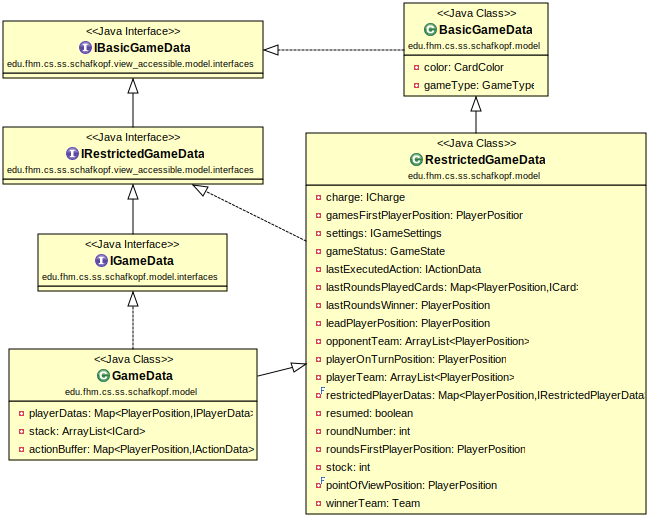
\includegraphics[width=1.0\textwidth]{./pictures/uml/class_diagram/uml_class_gamedata.pdf}
	\caption[Anwendung/Model -- Klassendiagramm Spieldaten]{Klassendiagramm der Spieldaten} \label{fig:model_gamedata}
\end{center}
\end{figure}

Im Folgenden findet sich eine Zusammenstellung der Datenelemente obiger Klassen mit Erklärung ihrer Bedeutung.

\textbf{\texttt{IBasicGameData}} und \textbf{\texttt{BasicGameData}} definieren Farbe und Typ des Spiels. Sie erhalten eine eigene Schnittstelle und Klasse, um angemeldete Spiele des Spielers definieren zu können, wofür die restlichen Informationen nicht benötigt werden.
\begin{itemize}
	\item \textbf{\texttt{color : CardColor}} Die Farbe des Spiels. Für farblose Spiele wie den Wenz steht hier \textbf{\texttt{null}}, für Solo und Farbwenz die Trumpffarbe und für das Sauspiel die Ruffarbe.
	\item \textbf{\texttt{gameType : GameType}} Der Typ des Spiels. (\autoref{sse:anwendung_model_enums})
\end{itemize}\bigskip

\textbf{\texttt{IRestrictedGameData}} und \textbf{\texttt{RestrictedGameData}} bieten alle Daten, die für jeden Spieler zugänglich sind.
\begin{itemize}
	\item \textbf{\texttt{charge : ICharge}} Informationen über Tarif und Spielwert.
	\item \textbf{\texttt{gamesFirstPlayerPosition : PlayerPosition}} Die Position des ersten Spielers eines neuen Spiels (\autoref{sse:anwendung_model_enums}). Wird im Anschluss ein nächstes Spiel gespielt, so inkrementiert sich diese.
	\item \textbf{\texttt{gameState : GameState}} Anhand des Spielzustands können die Spieler erfahren, was gerade von ihnen erwartet wird. (\autoref{sse:anwendung_model_enums})
	\item \textbf{\texttt{lastExecutedAction : IActionData}} Die letzte auf den Spieldaten ausgeführte Aktion. So wissen die Spieler, was die aktuellen Änderungen am Spiel herbeigeführt hat.
	\item \textbf{\texttt{lastRoundsPlayedCards : Map{\textless}PlayerPosition, ICard{\textgreater}}} Hier wird der letzte Stich, indiziert nach der Position der gespielten Karten, angezeigt. In der ersten Runde ist diese Map leer.
	\item \textbf{\texttt{lastRoundsWinner : PlayerPosition}} Die Position des Gewinners des letzten\newline
Stichs.
	\item \textbf{\texttt{leadPlayerPosition : PlayerPosition}} Die Position des Spielers, dessen angemeldetes Spiel gespielt wird.
	\item \textbf{\texttt{opponentTeam : List{\textless}PlayerPosition{\textgreater}}} Die Positionen der Spieler in der Gegnerpartei. Diese werden erst gesetzt, wenn die Teams sich offiziell kennen, also gesucht oder davongelaufen wurde, oder ein Solo gespielt wird.
	\item \textbf{\texttt{playerTeam : List{\textless}PlayerPosition{\textgreater}}} Die Positionen der Spieler in der Spielerpartei. Diese werden vervollständigt, wenn die Teams sich offiziell kennen. Der Spieler, dessen angemeldetes Spiel gespielt wird, ist von Anfang an bekannt und somit enthalten.
	\item \textbf{\texttt{playerOnTurnPosition : PlayerPosition}} Dieser Spieler ist am Zug, es wird eine Aktion von ihm erwartet. Es gibt bestimmte Ausnahmen, stoßen und Retour geben beziehen sich nicht darauf wer an der Reihe ist. Genauso kann man immer seine Absicht kundtun, gerne das nächste Spiel starten zu wollen.
	\item \textbf{\texttt{restrictedPlayerDatas : Map{\textless}PlayerPosition, IRestrictedPlayerData{\textgreater}}}\newline
Die Daten der Spieler mit eingeschränktem Zugriff, nicht einsehbar ist zum Beispiel die Hand des Spielers. Spielerdaten an der \textbf{\texttt{playerPointOfViewPosition}} sind allerdings immer vom Typ \textbf{\texttt{IPlayerData}}, also mit Vollzugriff und werden über Utility-Wrapper komfortabel zugänglich gemacht.
	\item \textbf{\texttt{resumed : boolean}} gibt an, ob das Spiel neu gestartet oder fortgeführt wurde.
	\item \textbf{\texttt{roundNumber : int}} Die Runde, in der sich das Spiel befindet. Ein neues Spiel beginnt bei -1. Dieser Wert ändert sich während der initialen Gebe- und Auswahlrunden nicht. Erst im Spielstatus \textbf{\texttt{PLAY}} beginnt der Zähler bei 0 und inkrementiert für jede neue Runde. Am Ende des Spiels ist er somit bei 7.
	\item \textbf{\texttt{stock : int}} Der Stock. Dieser wird nicht in \textbf{\texttt{charge}} gespeichert, weil das nur für die Tarifinformationen pro Spiel zuständig ist, der Stock aber über mehrere Spiele bestehen kann.
	\item \textbf{\texttt{pointOfViewPosition : PlayerPosition}} Die Position des Spielers, auf dessen Sicht diese Daten eingeschränkt sind. \textbf{\texttt{IRestrictedPlayerUtils}} verwendet diese Position, um die Spielerdaten mit uneingeschränkten Zugriff zu initialisieren.
	\item \textbf{\texttt{winnerTeam : Team}} Das Gewinner Team, sofern dieses bekannt ist. (\autoref{sse:anwendung_model_enums})
\end{itemize}\bigskip

\textbf{\texttt{IGameData}} und \textbf{\texttt{GameData}} enthalten die restlichen Informationen, die nicht für Views zugänglich sind. Auf diese darf nur vom Controller und Utilityklassen zugegriffen werden.

\begin{itemize}
	\item \textbf{\texttt{playerDatas : Map{\textless}PlayerPosition, IPlayerData{\textgreater}}} enthält alle Spielerdaten mit Vollzugriff.
	\item \textbf{\texttt{stack : List{\textless}ICard{\textgreater}}} Das Deck, bzw. der Stapel, von dem ausgeteilt wird.
	\item \textbf{\texttt{actionBuffer : Map{\textless}PlayerPosition, IActionData{\textgreater}}} Ein Puffer für Ak\-ti\-on\-en, die nicht sofort, sondern erst bei Zutreffen bestimmter Bedingungen aus\-ge\-führt oder validiert werden. Für den schnelleren Zugriff sind sie indiziert nach dem ausführenden Spieler.
\end{itemize}\bigskip

In folgenden Abschnitten wird auf die in den Spieldaten verwendeten Referenzklassen näher eingegangen.
%% Beschreiben des Playermodels
\subsubsection{Spielerdaten} \label{ssse:anwendung_model_player}

\begin{figure}[H]
\begin{center}
    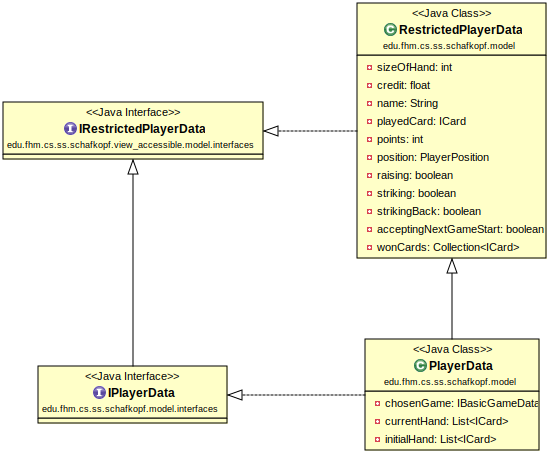
\includegraphics[width=0.9\textwidth]{./pictures/uml/class_diagram/uml_class_playerdata.pdf}
	\caption[Anwendung/Model -- Klassendiagramm Spielerdaten]{Klassendiagramm der Spielerdaten} \label{fig:model_player}
\end{center}
\end{figure}
Die Informationen über einzelne Spieler sind in den Spieler-Datenklassen enthalten.
Es gibt erneut eine eingeschränkte Version und eine mit Zugriff auf alle Informationen.

Auf die eingeschränkte Schnittstelle \textbf{\texttt{IRestrictedPlayerData}}, realisiert durch \textbf{\texttt{Res\-tric\-ted\-Pla\-yer\-Da\-ta}} erhalten alle Spieler Zugriff. Deshalb sind Informationen über den Inhalt der Hand eines Spielers, oder die Einzelheiten des angemeldeten Spiels, nicht zugänglich.\newline
Alles was man sich jedoch merken kann, also die gewonnenen Karten eines Spielers und seine Punkte, können eingesehen werden, um \acs{ki}-Spielern die Arbeit zu erleichtern. So müssen sie diese Informationen über das Spiel nicht selbst erneut speichern.\newline
Außerdem könnte es für eine View durchaus eine Option sein, diese Informationen für den Benutzer darzustellen, um ihm die Merk- und Denkarbeit zu erleichtern.

\begin{itemize}
	\item \textbf{\texttt{sizeOfHand : int}} hält die Anzahl der Karten auf der Hand. 
	\item \textbf{\texttt{credit : int}} Das aktuelle Vermögen des Spielers.
	\item \textbf{\texttt{name : String}} Der Name des Spielers.
	\item \textbf{\texttt{playedCard : ICard}} Die Karte, die von diesem Spieler gerade auf dem Tisch liegt.
	\item \textbf{\texttt{points : int}} Die Punkte des Spielers.
	\item \textbf{\texttt{position : PlayerPosition}} Die Position am Tisch. Diese sollte natürlich übereinstimmen mit der Position, über die die Spielerdaten in \textbf{\texttt{restrictedPlayerDatas}} bzw. \textbf{\texttt{playerDatas}} indiziert sind.
	\item \textbf{\texttt{raising / striking / strikingBack / acceptingNextGameStart : boolean}} Geben an, ob der Spieler gelegt, gestoßen, Retour gegeben oder den Start des nächsten Spiels akzeptiert hat.
	\item \textbf{\texttt{wonCards: Collection{\textless}ICard{\textgreater}}} Die gewonnen Karten im aktuell laufenden Spiel.
\end{itemize}\bigskip

\textbf{\texttt{IPlayerData}} und \textbf{\texttt{PlayerData}} enthalten die restlichen Informationen. Ein Spieler bekommt über die Utility-Wrapper (\autoref{sse:anwendung_model_utility}) Zugriff auf diese Schnittstelle, aber nur auf seine eigenen Spielerdaten und nicht auf die der Mitspieler.

\begin{itemize}
	\item \textbf{\texttt{chosenGame : IBasicGameData}} Enthält neben dem Typ auch die Farbe des angemeldeten Spiels.
	\item \textbf{\texttt{currentHand : List{\textless}ICard{\textgreater}}} Die aktuelle Hand des Spielers, die unter anderem zur Validierung von Aktionen verwendet wird.
	\item \textbf{\texttt{initialHand : List{\textless}ICard{\textgreater}}} Die Starthand des Spielers. Sie wird verwendet, um am Ende des Spiels die Laufenden zu berechnen.
\end{itemize}

\clearpage

%% Beschreiben des Tarif Models
\subsubsection{Tarifdaten} \label{ssse:anwendung_model_charge}

\begin{figure}[H]
\begin{center}
    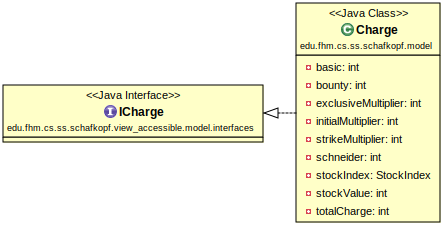
\includegraphics[width=0.9\textwidth]{./pictures/uml/class_diagram/uml_class_charge.pdf}
	\caption[Anwendung/Model -- Klassendiagramm Tarifdaten]{Klassendiagramm der Tarifdaten} \label{fig:model_charge}
\end{center}
\end{figure}

\textbf{\texttt{ICharge}} und \textbf{\texttt{Charge}} definieren den Tarif eines Spiels. Die Bezeichnungen aus \autoref{sse:grundlagen_schafkopf_tarif} finden sich hier wieder. Es ist zu unterscheiden zwischen Werten, die sich bereits während des Spielverlaufs ändern -- wie \textbf{\texttt{strikeMultiplier}} -- und solchen, die nur am Ende des Spiels gesetzt sind -- wie \textbf{\texttt{totalCharge}}.
\begin{itemize}
	\item \textbf{\texttt{basic : int}} Grundtarif.
	\item \textbf{\texttt{bounty : int}} Prämientarif/Zähleinheit. Das entspricht der Anzahl der Laufenden für ein Team.
	\item \textbf{\texttt{schneider : int}} Leistungstarif/Zähleinheit.
	\item \textbf{\texttt{initialMultiplier : int}} gibt an, wie oft gelegt wurde.
	\item \textbf{\texttt{strikeMultiplier : int}} gibt an, wie oft gestoßen wurde.
	\item \textbf{\texttt{exclusiveMultiplier : int}} 1 bei exklusiven Spielen, sonst 0.
	\item \textbf{\texttt{stockIndex : StockIndex}} Dieser gibt an, wie in am Ende des Spiels mit dem Stock verfahren wird. (\autoref{sse:anwendung_model_enums})
	\item \textbf{\texttt{stockValue : int}} Der Wert, den jeder Spieler in den Stock einzahlen muss, bzw. ausgezahlt bekommt.
	\item \textbf{\texttt{totalCharge : int}} Der Gesamttarif für das Spiel in Cent.	
\end{itemize}

\clearpage

%% Beschreiben des Spielkarten Models
\subsubsection{Spielkartendaten} \label{ssse:anwendung_model_card}

\begin{figure}[H]
\begin{center}
    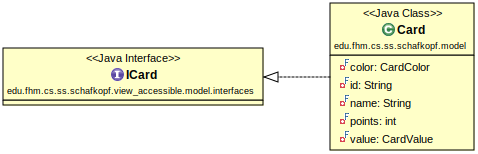
\includegraphics[width=0.9\textwidth]{./pictures/uml/class_diagram/uml_class_card.pdf}
	\caption[Anwendung/Model -- Klassendiagramm Spielkartendaten]{Klassendiagramm einer Spielkarte} \label{fig:model_card}
\end{center}
\end{figure}

\textbf{\texttt{ICard}} und \textbf{\texttt{Card}} repräsentieren eine Spielkarte. Diese ist immutable, ihre Werte lassen sich also nach Erstellung nicht mehr verändern.
\begin{itemize}
	\item \textbf{\texttt{color: CardColor}} Die Farbe der Karte. (\autoref{sse:anwendung_model_enums})
	\item \textbf{\texttt{value: CardValue}} Der Zahlwert der Karte. (\autoref{sse:anwendung_model_enums})
	\item \textbf{\texttt{id: String}} Ein eindeutiger Identifier, bestehend aus dem Anfangsbuchtaben der Farbe und des Werts, welche in deren Enums hinterlegt sind. Eichel Sau ist z.B. "'es"', Herz Zehn "'h1"'.
	\item \textbf{\texttt{name : String}} Der vollständige Name der Karte. Er wird generiert aus den Namen von Farbe und Wert, die ebenfalls in den Enums definiert sind.
	\item \textbf{\texttt{points : int}} Die Augen der Karte. Sie werden aus dem Zahlwert generiert.
\end{itemize}

\clearpage

%% Beschreiben des Aktionsdaten Models
\subsubsection{Aktionsdaten} \label{ssse:anwendung_model_actions}

\begin{figure}[H]
\begin{center}
    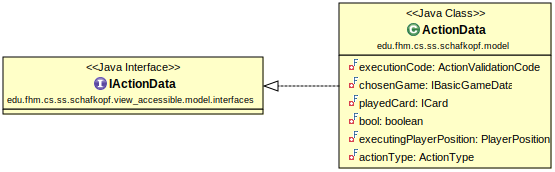
\includegraphics[width=1.0\textwidth]{./pictures/uml/class_diagram/uml_class_actiondata.pdf}
	\caption[Anwendung/Model -- Klassendiagramm Aktionsdaten]{Klassendiagramm der Aktionsdaten} \label{fig:model_actions}
\end{center}
\end{figure}

\textbf{\texttt{IActionData}} und \textbf{\texttt{ActionData}} realisieren einen Container für Aktionsdaten. Die Schnittstelle bietet Lesezugriff auf alle Daten der Aktion. Dabei werden solche, die für die Aktion nicht relevant sind mit \textbf{\texttt{null}} oder Default Werten belegt. Eine Aktion für das Spielen einer Karte enthält z.B. keine Information über ein gewähltes Spiel.

\begin{itemize}
	\item \textbf{\texttt{executionCode: ActionValidationCode}} Der Code, mit dem die Aktion aus\-ge\-führt oder abgewiesen wurde (\autoref{sse:anwendung_model_enums}). Dieser sollte \textbf{\texttt{EXE\-CU\-TED{\_}CHAN\-GES}} sein für Aktionen, die erfolgreich auf den Spieldaten aus\-ge\-führt wurden und für abgewiesene Aktionen der Fehlercode. Der Code abgewiesener Aktionen ist primär für die Testumgebung von Bedeutung.
	\item \textbf{\texttt{actionType : ActionType}} enthält einen repräsentativen Bezeichner für den Typ der Aktion. (\autoref{sse:anwendung_model_enums})
	\item \textbf{\texttt{chosenGame : IBasicGameData}} Dieser Wert sollte nur für Aktionen vom Typ \textbf{\texttt{CHOOSE}} gesetzt sein und enthält das angemeldete Spiel des Spielers.
	\item \textbf{\texttt{bool : boolean}} ist relevant für alle Aktionen, die einen Wahrheitswert benötigen, wie \textbf{\texttt{STRIKE}} und \textbf{\texttt{STRIKEBACK}}.
	\item \textbf{\texttt{executingPlayerPosition : Playerposition}} Die Position des Spielers, der die Aktion ausgeführt hat.
\end{itemize}

\clearpage

%% Beschreiben der Enums
\subsection{Aufzählungstypen} \label{sse:anwendung_model_enums}
Um die Datenhaltung anschaulicher zu gestalten wurden eine Reihe von Aufzählungstypen erstellt. Die Bedeutungen der Enum-Klassen werden in diesem Abschnitt erklärt.

\textbf{\texttt{ActionType}} definiert den Typ einer Aktion und wird verwendet, um Aktionsdaten zu unterscheiden.
\begin{itemize}
	\item \textbf{\texttt{GET}} Karten geben.
	\item \textbf{\texttt{PLAY}}	Eine Karte spielen.
	\item \textbf{\texttt{RAISE}} Legen.
	\item \textbf{\texttt{STRIKE}} Stoßen.
	\item \textbf{\texttt{CHOOSE}} Ein Spiel anmelden oder auch passen.
	\item \textbf{\texttt{STRIKEBACK}} Retour geben.
	\item \textbf{\texttt{NEXTGAMEACCEPTED}} Den Start des nächsten Spiels akzeptieren.
	\item \textbf{\texttt{NEXTGAMESTARTED}} Das nächste Spiel wurde gestartet.
\end{itemize}\bigskip

\textbf{\texttt{ActionValidationCode}} gibt Auskunft darüber, ob eine Aktion erfolgreich durchgeführt wurde oder warum nicht. Er wird vom Gamecontroller verwendet um dem Spieler Informationen bezüglich der weiteren Verarbeitung seiner eingereichten Aktion zurückzugeben. Er wird außerdem in \textbf{\texttt{ActionData}} hinterlegt und spielt eine Rolle in der Testumgebung.
\begin{itemize}
	\item \textbf{\texttt{CARD{\_}NOTALLOWED}} Die gespielte Karte ist nicht erlaubt.
	\item \textbf{\texttt{CHOOSE{\_}COLORNOTALLOWED}} Die gewählte Farbe eines angemeldeten Spiels ist nicht erlaubt.
	\item \textbf{\texttt{CHOOSE{\_}TYPENOTALLOWED}} Der gewählte Spieltyp eines angemeldeten Spiels ist nicht erlaubt.
	\item \textbf{\texttt{GET{\_}HANDFULL}} Der Spieler hat keine Karten mehr bekommen, da seine Hand voll ist.
	\item \textbf{\texttt{ID{\_}INVALID}} Die Spieler ID ist ungültig.
	\item \textbf{\texttt{RAISE{\_}ALREADYRAISED}} Der Spieler hat bereits gelegt.
	\item \textbf{\texttt{RAISE{\_}TOOMUCHCARDS}} Der Spieler hat zu viele Karten um zu legen.
	\item \textbf{\texttt{REQUIRED{\_}DATA{\_}CORRUPT}} Daten, die benötigt werden um die Aktion durchzuführen sind ungültig. Dieser Code weist auf Fehler in der Datenhaltung hin.
	\item \textbf{\texttt{STATE{\_}WRONG}} Die Aktion darf in diesem Spielstatus nicht ausgeführt werden.
	\item \textbf{\texttt{STRIKE{\_}ALREADYSTRUCK}} Der Spieler hat bereits gestoßen.
	\item \textbf{\texttt{STRIKE{\_}NOTOPPONENT}} Der Spieler darf nicht stoßen, wenn er nicht im Gegnerteam ist.
	\item \textbf{\texttt{STRIKEBACK{\_}ALREADYSTRUCKBACK}} Der Spieler hat bereits Retour gegeben.
	\item \textbf{\texttt{STRIKEBACK{\_}NOTPLAYER}} Nur der Spieler, der das Spiel angemeldet hat, darf Retour geben.
	\item \textbf{\texttt{VALIDATION{\_}SUCCESS}} Die Validierung der Aktion war erfolgreich. Dieser Wert ist nur für den Gamecontroller von Bedeutung und sollte nicht an den Spieler ausgeliefert werden.
	\item \textbf{\texttt{EXECUTED{\_}CHANGES}} Die Aktion wurde erfolgreich durchgeführt und Änderungen an den Spieldaten vorgenommen.
	\item \textbf{\texttt{EXECUTED{\_}NOCHANGES}} Die Aktion wurde entgegengenommen, hat aber zu keinen Änderungen der Spieldaten geführt.
	\item \textbf{\texttt{TURN{\_}NOTONTURN}} Der Spieler ist nicht am Zug.
	\item \textbf{\texttt{STARTNEXT{\_}ALREADYACCEPTING}} Der Spieler akzeptiert bereits den Start des nächs\-ten Spiels.
\end{itemize}\bigskip

\textbf{\texttt{CardColor}} definiert die Farbe einer Karte und wird verwendet um Karten, die Trumpffarbe und anderes zu beschreiben. Jede Farbe hat zusätzliche Attribute.

\begin{itemize}
	\item \textbf{\texttt{id : String}} Ein eindeutiger Identifier. Der erste Buchstabe der Farbe.
	\item \textbf{\texttt{name : String}} Der Name der Farbe.
	\item \textbf{\texttt{number : int}} Der Wert der Farbe. Dieser wird zum Vergleich der Karten im \textbf{\texttt{CardComparator}} verwendet.
	\item \textbf{\texttt{EICHEL}} Die Farbe Eichel.
	\item \textbf{\texttt{GRAS}}	Die Farbe Gras.
	\item \textbf{\texttt{HERZ}} Die Farbe Herz.
	\item \textbf{\texttt{SCHELLN}} Die Farbe Schelln.
\end{itemize}\bigskip

\textbf{\texttt{CardValue}} definiert den Zahlenwert einer Karte und wird ausschließlich dafür verwendet. Jeder Wert hat zusätzliche Attribute.

\begin{itemize}
	\item \textbf{\texttt{id : String}} Ein eindeutiger Identifier. Der erste Buchstabe oder die erste Ziffer des Werts.
	\item \textbf{\texttt{name : String}} Der Name der Werts.
	\item \textbf{\texttt{number : int}} Der Wert des Zahlwerts. Dieser wird zum Vergleich der Karten im \textbf{\texttt{CardComparator}} verwendet.
	\item \textbf{\texttt{points : int}} Die Augen des Werts.
	\item \textbf{\texttt{SAU}} Die Sau.
	\item \textbf{\texttt{ZEHN}}	Die Zehn.
	\item \textbf{\texttt{KÖNIG}} Der König.
	\item \textbf{\texttt{...}} usw.
	\item \textbf{\texttt{SIEBEN}} Die Sieben.
\end{itemize}\bigskip

\textbf{\texttt{GameState}} definiert den Zustand, in dem sich ein laufendes Spiel gerade befindet. Die Spieler können aus diesem erkennen, was sie zu tun haben. Die Aufzählung ist in der Reihenfolge, wie die Zustände während eines Spielablaufs auftreten.

\begin{itemize}
	\item \textbf{\texttt{GET{\_}RAISE}} Die ersten beiden Runden, in denen sich die Spieler Karten geben lassen und legen können.
	\item \textbf{\texttt{CHOOSE}} Eine Runde, in der ein Spiel angemeldet oder gepasst werden kann.
	\item \textbf{\texttt{PLAY}} Die acht Runden, in denen Karten gespielt werden.
	\item \textbf{\texttt{STRIKE}} Von den Gegenspielern wird erwartet, anzugeben, ob sie stoßen wollen.
	\item \textbf{\texttt{STRIKEBACK}} Ein gestoßener Spieler muss ansagen, ob er Retour gibt.
	\item \textbf{\texttt{FINISHED}} Das Spiel ist beendet und Informationen, wie kompletter Tarif, Anzahl der Laufenden des Teams und weitere, stehen zur Verfügung.
\end{itemize}\bigskip

\textbf{\texttt{GameType}} Definiert verschiedene Spieltypen, die angemeldet und gespielt werden können. Da für jeden Typ unterschiedliche Spielregeln gelten (\autoref{se:grundlagen_schafkopf}) wird sich während des gesamten Spielverlaufs darauf bezogen, z.B. um Züge zu validieren. Jeder Typ hat eigene Attribute. Es wird noch eine Methode \textbf{\texttt{dominates(GameType)}} angeboten, mit der zwei Typen verglichen werden können. Diese Funktion ist für die Auswahlphase des Spiels wichtig.

\begin{itemize}
	\item \textbf{\texttt{isExclusive : boolean}} Das Spiel ist exklusiv.
	\item \textbf{\texttt{isPartnerGame : boolean}} Ein Partnerspiel.
	\item \textbf{\texttt{isWenz : boolean}} Ein Wenz.
	\item \textbf{\texttt{needsColor : boolean}} Der Typ benötigt zum Anmelden eine Farbe. Wenze kann man ohne Farbe anmelden.
	\item \textbf{\texttt{weight : int}} Das Gewicht des Spieltyps. Dieses wird in \textbf{\texttt{dominates(GameType)}} verwendet, um die Typen zu vergleichen.
	\item \textbf{\texttt{name : String}} Der Name des Spieltyps.
	\item \textbf{\texttt{WENZ}} Der Wenz.
	\item \textbf{\texttt{WENZ{\_}TOUT}} Der Wenz Tout.
	\item \textbf{\texttt{SAUSPIEL}} Das Sauspiel.
	\item \textbf{\texttt{SOLO}} Das Solo.
	\item \textbf{\texttt{PASS}} Passen.
	\item \textbf{\texttt{...}} usw.
\end{itemize}\bigskip

\textbf{\texttt{PlayerPosition}} beschreibt die Position eines Spielers auf dem Spielfeld. In der Regel sitzen sich beim Schafkopf jeweils zwei Spieler gegenüber, daraus resultieren die vier Positionen. Es wird eine Methode \textbf{\texttt{getNext()}} angeboten, die die im Uhrzeigersinn nächste Position liefert, sowie \textbf{\texttt{getBefore()}}, die gegen den Uhrzeigersinn Nächste. Spieler werden in der Anwendung meist über ihre Position angesprochen und indiziert.

\begin{itemize}
	\item \textbf{\texttt{BOTTOM}} Unterer Spieler.
	\item \textbf{\texttt{LEFT}}	Linker Spieler.
	\item \textbf{\texttt{TOP}} Oberer Spieler.
	\item \textbf{\texttt{RIGHT}} Rechter Spieler.
\end{itemize}\bigskip

\textbf{\texttt{Stockindex}} gibt an, wie am Ende einer Runde mit dem Stock verfahren wird.

\begin{itemize}
	\item \textbf{\texttt{DOUBLE}} Das Spielerteam doppelt auf.
	\item \textbf{\texttt{PAY{\_}IN}} Es wird eingezahlt (alle haben gepasst).
	\item \textbf{\texttt{PAY{\_}OUT}} Der Stock wird an die Spielerpartei ausgezahlt. 				
	\item \textbf{\texttt{IGNORE}} Der Stock bleibt unverändert.
\end{itemize}\bigskip

\textbf{\texttt{Team}} definiert \textbf{\texttt{PLAYER{\_}TEAM}} und \textbf{\texttt{OPPONENT{\_}TEAM}}. Teams können darüber indiziert und angesprochen werden.

\clearpage

%% Beschreiben der Utility-Wrapper
\subsection{Utility-Wrapper} \label{sse:anwendung_model_utility}
Die Utility-Wrapper bieten eine Reihe an Funktionalität für Spieler und Controller, um komplexere Zugriffe auf das Datenmodell durchzuführen.
So ist gewährleistet, dass die Zugriffsabfolgen nicht mehrfach programmiert werden, was den Wartungs- und Änder\-ungs\-aufwand genauso wie die Fehleranfälligkeit, verringert.

Das Diagramm gibt wieder einen Überblick über die verschiedenen Klassen und Interfaces. Die Methoden sind der Übersichtlichkeit halber nicht dargestellt und werden im Anschluss erklärt.

\begin{figure}[H]
\begin{center}
    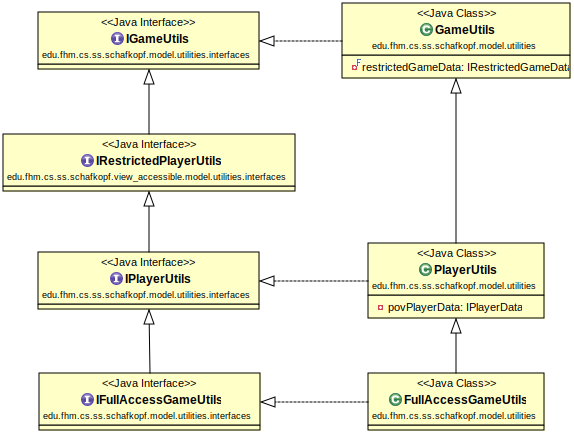
\includegraphics[width=1.0\textwidth]{./pictures/uml/class_diagram/uml_class_utilitywrapper.pdf}
	\caption[Anwendung/Model -- Klassendiagramm Utility-Wrapper]{Klassendiagramm der Utility-Wrapper} \label{fig:model_utilitywrapper}
\end{center}
\end{figure}

Die Utilities gliedern sich in Klassen logisch zusammenhängender Zugriffe. Durch verschiedene verknüpfte Schnittstellen werden außerdem Zugriffsebenen angeboten, die die Bedürfnisse und Rechte der verwendenden Klassen widerspiegeln. So wird Spielaktionen und Kontrolleinheiten voller Zugriff auf Lese- und Schreibfunktionen, Spielern hingegen nur eingeschränkter Zugriff auf Lesefunktionen geboten. Die Spieler dürften die Spieldaten zwar manipulieren, da sie nur eine Kopie besitzen, erhalten aber dennoch keinen Zugriff auf viele Methoden. Diese sind entweder nicht relevant für sie, oder benötigen Schnittstellen, die dem Spieler nicht zur Verfügung stehen. Die angebotene Schnittstelle wird so übersichtlicher.

\textbf{\texttt{IGameUtils}} und \textbf{\texttt{GameUtils}} bieten generelle, spielerunabhängige Informationen. Die Klasse erhält mit \textbf{\texttt{restrictedGameData : IRestrictedGameData}} eine Referenz auf eingeschränkte Spieldaten. Eingeschränkt, da sichergestellt werden soll, dass keine Zugriffe auf Informationen erfolgen, die über die \textbf{\texttt{IRestrictedGameData}} Schnittstelle hinausgehen.
\begin{itemize}
	\item \textbf{\texttt{calculatePointsOfCards(Collection{\textless}ICard{\textgreater})}} summiert die Punkte der gegebenen Karten.
	\item \textbf{\texttt{dominates(ICard, ICard)}} leitet den Aufruf weiter an einen, auf die Spieldaten zugeschnittenen \textbf{\texttt{CardComparator}} und gibt true zurück, wenn die zweite Karte höher ist als die erste.
	\item \textbf{\texttt{getCardsOnTable()}} gibt alle auf dem Tisch liegenden Karten zurück. Das sind die gespielten Karten der Spieler.
	\item \textbf{\texttt{getFirstPlayedCard()}} gibt die erste gespielte Karte der Runde zurück.
	\item \textbf{\texttt{getRestrictedGameData()}} liefert die Referenz der eingeschränkten Spieldaten, auf denen die Utilityklasse arbeitet.
	\item \textbf{\texttt{getTeamsPoints(Team)}} berechnet die Punkte eines Teams, soweit dieses  bekannt ist.
	\item \textbf{\texttt{getTeamsWonCards(Team)}} liefert eine Sammlung aller gewonnene Karten eines Teams, soweit dieses bekannt ist.
	\item \textbf{\texttt{getTotalMultiplier()}} berechnet den Multiplikator des Spielwerts aus den Tarifinformationen.
	\item \textbf{\texttt{getTrumpColor([ $\epsilon$ $\mid$ IBasicGameData ])}} liefert die aktuelle (für die eigene Referenz auf die Spieldaten) Trumpffarbe, oder die des Parameters. (2-fach überladen)
	\item \textbf{\texttt{haveAllPlayersPlayedCard())}} liefert \textbf{\texttt{true}}, wenn in dieser Runde alle Spieler ihre Karte gespielt haben.
	\item \textbf{\texttt{isCardHighTrump([ $\epsilon$ $\mid$ GameType $\mid$ IBasicGameData ], ICard)}} gibt zurück, ob die Karte aktuell, oder für gegebenen Parameter einer der Herren ist. (3-fach überladen)
	\item \textbf{\texttt{isCardTrump([ $\epsilon$ $\mid$ IBasicGameData ], ICard)}} gibt zurück, ob die Karte aktuell oder für gegebenen Parameter Trumpf ist. (2-fach überladen)
	\item \textbf{\texttt{isMateSearchedThisRound()}} beantwortet die Frage, ob der Partner des Spielers in dieser Runde gesucht wurde. Diese Methode aufzurufen ergibt nur Sinn, wenn das aktuelle Spiel ein Sauspiel ist. Sonst liefert sie immer false.
\end{itemize}\bigskip

\textbf{\texttt{PlayerUtils}} erweitert obige Funktionalität nun um Informationen, die die Spielerdaten mit einbeziehen. Die zwei realisierten Interfaces trennen die Methoden in solche, die nur Informationen über einen bestimmten Spieler (\textbf{\texttt{IRestrictedPlayerUtils}}) bieten und solche, die mit einem beliebigen Spieler als Parameter aufgerufen werden können (\textbf{\texttt{IPlayerUtils}}).\newline
Um uneingeschränkte Daten über einen spezifischen Spieler anbieten zu können, erhält \textbf{\texttt{PlayerUtils}} im Konstruktor eine Referenz auf ein Spielerdaten-Objekt, welche in \textbf{\texttt{pov\-Player\-Data}} gespeichert wird, "'pov"' steht für Point-Of-View.\newline
Die Methoden der beide Schnittstellen realisierenden Klasse sind somit mindestens zweifach überladen, um den Anforderungen von \textbf{\texttt{IPlayerUtils}} gerecht zu werden.
Wird eine Methode mit Spielerdaten als Parameter aufgerufen so wird die Information über diese zurückgegeben, sonst über die Daten in \textbf{\texttt{povPlayerData}}. Die eingeschränkte Schnittstelle ist für die Verwendung von Playerviews gedacht, die nur vollen Zugriff auf ihre eigenen Daten haben.

Auf die Angabe der Überladung mit beliebigen Spielerdaten wird, der Über\-sicht\-lich\-keit halber, in der Liste der Methoden verzichtet.
\begin{itemize}
	\item \textbf{\texttt{calculateHighCardsInRow([ $\epsilon$ $\mid$ IBasicGameData ])}} berechnet die Anzahl der Laufenden eines Spielers, für ein gegebenes oder das aktuelle Spiel. (4-fach über\-la\-den)
	\item \textbf{\texttt{countColor([ $\epsilon$ $\mid$ IBasicGameData ], CardColor)}} zählt die Anzahl einer gegebenen Farbe in der Hand des Spielers, für das aktuelle oder ein gegebenes Spiel. Es wird jede Karte dieser Farbe gezählt -- also auch die Trumpffarbe -- außer sie gehört zu den Herren. (5-fach überladen)
	\item \textbf{\texttt{countTrump([ $\epsilon$ $\mid$ IBasicGameData ])}} zählt die Anzahl der Trumpfkarten in der Hand des Spielers, für das aktuelle oder ein gegebenes Spiel. (3-fach überladen)
	\item \textbf{\texttt{getAllColorCards([ $\epsilon$ $\mid$ IBasicGameData ], CardColor)}} gibt eine Sammlung der Karten einer bestimmten Farbe in der Hand des Spielers zurück, für das aktuelle oder ein gegebenes Spiel. (4-fach überladen)
	\item \textbf{\texttt{getAvailableCards()}} gibt eine Sammlung der Karten in der Hand eines Spielers zurück, die er bei aktuellem Spielstand spielen kann. Diese Methode ist relativ komplex und verwendet einige der anderen Utility-Methoden. Sie beachtet den Trumpf- und Farbzwang, Davonlaufen und Zugeben der Rufsau. Außerdem wird überprüft, ob sich das Spiel im richtigen Zustand befindet. Falls die Spieldaten korrupt sind, wird eine leere Sammlung zurückgegeben. (2-fach überladen)
	\item \textbf{\texttt{getAvailableColors(GameType)}} gibt eine Sammlung der Farben zurück, mit denen ein Spiel des gegebenen Typen angemeldet werden kann. Der Aufruf dieser Methode ist für die Auswahlphase des Spiels gedacht. Falls das Spiel sich im falschen Zustand befindet wird eine leere Sammlung zurückgegeben. (2-fach überladen)
	\item \textbf{\texttt{getAvailableGameTypes()}} gibt eine Sammlung der Spieltypen zurück, mit denen ein Spiel angemeldet werden kann. Der Aufruf dieser Methode ist ebenso für die Auswahlphase des Spiels gedacht. (2-fach überladen)	
	\item \textbf{\texttt{getChooseGameValidationCode(IBasicGameData)}} liefert einen \textbf{\texttt{Action\-Va\-li\-da\-tion\-Code}} zurück, dem entnommen werden kann, ob ein angemeldetes Spiel erlaubt ist oder warum nicht (\autoref{sse:anwendung_model_enums}). Diese Methode ist nur über die \textbf{\texttt{IPlayer\-Utils}} Schnittstelle zugänglich und für die Validierung von Aktionen gedacht. 
	\item \textbf{\texttt{isAllowedToChooseGame(IBasicGameData $\mid$ GameType, CardColor)}} ist die  vereinfachte, über \textbf{\texttt{IRestrictedPlayerData}} zugängliche Version obiger Methode, die nur einen Wahrheitswert zurückgibt. Diese Struktur findet sich in folgenden Methoden wieder. (2-fach überladen)
	\item \textbf{\texttt{getGetCardsValidationCode()}} und \textbf{\texttt{isAllowedToGetCards()}} geben zurück, ob es dem Spieler erlaubt ist, sich Karten geben zu lassen.
	\item \textbf{\texttt{getPlayCardValidationCode(ICard)}} und \textbf{\texttt{isAllowedToPlayCard(ICard)}} geben zurück, ob der Spieler die gewählte Karte spielen darf.
	\item \textbf{\texttt{getRaiseValidationCode()}} und \textbf{\texttt{isAllowedToRaise()}} geben zurück, ob der Spieler legen darf.
	\item \textbf{\texttt{getStrikeValidationCode()}} und \textbf{\texttt{isAllowedToStrike()}} geben zurück, ob der Spieler stoßen darf.
	\item \textbf{\texttt{getStrikeBackValidationCode()}} und \textbf{\texttt{isAllowedToStrikeBack()}} geben zurück, ob der Spieler Retour geben darf.	
	\item \textbf{\texttt{isColorAllowedToChoose(GameType, CardColor)}} gibt zurück, ob die Kombination aus Farbe und Spieltyp erlaubt ist.
	\item \textbf{\texttt{isGameTypeAllowedToChoose()}} gibt zurück, ob ein gegebener Spieltyp erlaubt ist. Diese Methode bezieht den aktuell angemeldeten Spieltypen mit ein. Der Gegebene muss diesen dominieren, um erlaubt zu sein. Außerdem wird über\-prüft ob die Voraussetzungen an die Hand des Spielers erfüllt sind.		
	\item \textbf{\texttt{isExpectedToAct()}} liefert die Information, ob von einem Spieler erwartet wird, einen Zug zu machen. Dies ist vor allem für die \acs{ki}-Spieler interessant, da sie nur dann aktiv werden müssen.	
	\item \textbf{\texttt{isHandFull()}} gibt zurück, ob die Hand des Spielers vollständig ist. Dazu wird mit einem in \textbf{\texttt{IRestrictedGameData}} hinterlegten statischen Wert verglichen, normalerweise 8.
	\item \textbf{\texttt{isLeadplayerMate()}} liefert die Information, ob bei einem angemeldeten Rufspiel ein Spieler als Partner in der Spielerpartei ist.
	\item \textbf{\texttt{isOnTurn()}} Ist der Spieler an der Reihe?
	\item \textbf{\texttt{ownsCard(ICard)}} prüft, ob sich die Karte in der Hand des Spielers befindet.
\end{itemize}\bigskip

Die bisherigen Utility-Wrapper haben Lesezugriff auf den Spieldaten angeboten. \textbf{\texttt{IFull\-Ac\-cess\-Pla\-yer\-Ut\-ils}} wird realisiert durch \textbf{\texttt{FullAccessPlayerUtils}} und definiert Funktionen, die komplexe Folgen von Schreibzugriffen umsetzen. Andere liefern zwar Daten, sollen aber für Playerviews nicht zugänglich sein.
Dafür wird voller Zugriff auf die Spieldaten benötigt. Bei der Instantiierung wird deshalb eine Referenz auf \textbf{\texttt{IGameData}} übergeben. Die privaten Methoden werden hier nicht aufgeführt, sie dienen der Aufteilung der Funktionalität in zusammenhängende, wiederverwendbare Teile und werden von den anderen Methoden verwendet.
\begin{itemize}
	\item \textbf{\texttt{calculateBasicChargeForCurrentGame()}} berechnet den Grundtarif für das Spiel mit den Einstellungen aus den Spieldaten. Diese Methode ist hier untergebracht, weil die Spieler über das Charge Datenobjekt an diese Information kommen und sie nicht selbst berechnen müssen.
	\item \textbf{\texttt{calculateWinnerCardPosition()}} berechnet, wer den aktuell auf dem Tisch liegenden Stich dominiert.
	\item \textbf{\texttt{clearPlayedCards()}} setzt die gespielten Karten der Spieler auf \textbf{\texttt{null}}.
	\item \textbf{\texttt{dealCardsFromStack(IPlayerData, int)}} gibt dem Spieler eine Anzahl Karten auf die Hand.
	\item \textbf{\texttt{endGameManipulations()}} ist eine komplexere Schreibfunktion, die am Ende eines Spiels aufgerufen wird. Sie berechnet und befüllt den Gewinner des Spiels, fehlende Tarifinformationen, wie Laufende des Teams, Stock, Schneider und Gesamttarif und teilt Spielwert und Stock unter den Spielern auf. Der Spielstatus wird am Ende auf \textbf{\texttt{FINISHED}} gesetzt.
	\item \textbf{\texttt{fillOpponentTeam()}} jeder Spieler, der nicht im Spielerteam ist, wird mit Aufruf dieser Methode ins Gegnerteam gesteckt. Das Spielerteam sollte dabei vollständig befüllt, das Gegnerteam leer sein, wenn nicht kommt es zu Inkonsistenz.
	\item \textbf{\texttt{getGameData()}} liefert eine Referenz auf die Spieldaten mit uneingeschränktem Zugriff.
	\item \textbf{\texttt{haveAllPlayersChosen()}} überprüft, ob in allen Spielerdaten \textbf{\texttt{chosenGame}} gesetzt ist.
	\item \textbf{\texttt{initializeGameData(PlayerPosition, [ $\epsilon$ $\mid$ List{\textless}ICard{\textgreater} ])}} \newline 
ini\-tia\-li\-siert die Spieldaten für das nächste Spiel. Die gegebene Spielerposition wird der erste Spieler des Spiels. Der optionale Parameter kann verwendet werden, um das Spiel mit einem vordefinierten Kartenstapel zu initialisieren. Ist dieser nicht gesetzt so wird ein neuer, gemischter Stapel verwendet.
	\item \textbf{\texttt{initializePlayerData(IPlayerData)}} initialisiert gegebene Spielerdaten. Diese Methode wird in obiger verwendet.
	\item \textbf{\texttt{startGameManipulations()}} wird aufgerufen, um nach der Auswahlphase das Spiel zu starten. Die Karten der Spieler werden sortiert und Informationen wie Spieltyp, Farbe und -- falls bereits bekannt -- die Parteien in die Spieldaten geschrieben.
\end{itemize}\bigskip

Die Utility-Wrapper sind recht nützlich und durch die verschiedenen Schnittstellen auf die unterschiedlichen Anwendungbereiche zugeschnitten. Sie vereinfachen den Code im Rest der Anwendung enorm.\bigskip

Zwei weitere Klassen vervollständigen die Utilites der Anwendung.

Die Logik rund um den Kartenstapel ist in in \textbf{\texttt{StackHandler}} verpackt. Dieser generiert zufällige oder vorgegebene Kartenstapel und bietet schnellen Zugriff auf eine Karte über deren \textbf{\texttt{id}}. Das Interface dazu ist \textbf{\texttt{IStackHandler}}.

\textbf{\texttt{CardComparator}} erbt von \textbf{\texttt{Comparator}}, einer von Java in \textbf{\texttt{java.util}} zur Verfügung gestellten Klasse. Er stellt die Karten abhängig von Spieltyp und Trumpffarbe in Relation zueinander. Mit ihm können Karten komfortabel sortiert und verglichen werden. Dabei muss beachtet werden, dass durch den Comparator eine totale Ordnung über den Karten definiert wird. Es kommen zuerst die Herren, anschließend die weiteren Trumpfkarten und zum Schluss die restlichen Farbkarten. Von \textbf{\texttt{CardComparator}} wird nicht beachtet, dass eine Farbe nur von der gleichen Farbe gestochen werden kann. Dies muss beim konkreten Vergleich von zwei Karten noch zusätzlich überprüft werden.

\clearpage

%% Beschreiben Settingsmodels
\subsection{Settingsmodel} \label{sse:anwendung_model_settings}
Die Spieleinstellungen enthalten Informationen, die für die Berechnung des Tarifs und das Erstellen eines neuen Spiels von Bedeutung sind. Beim Instanziieren von neuen Spieldaten werden diese als Parameter übergeben. Jedes Spiel erhält eine Referenz auf die Einstellungen mit denen es erstellt wurde, damit diese auch beim Fortführen eines Spiels verfügbar sind.
Die \textbf{\texttt{IGameSettings}} Schnittstelle bietet Lese- und Schreibzugriff auf die \textbf{\texttt{GameSettings}} an, \textbf{\texttt{IPrimitiveGameSettings}} nur Lesezugriff.

\begin{figure}[H]
\begin{center}
    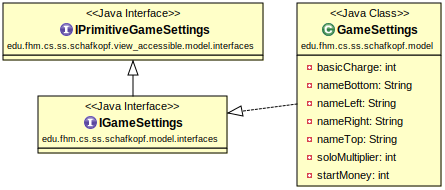
\includegraphics[width=0.8\textwidth]{./pictures/uml/class_diagram/uml_class_settings.pdf}
	\caption[Anwendung/Model -- Klassendiagramm Spieleinstellungen]{Klassendiagramm der Spieleinstellungen} \label{fig:model_settings}
\end{center}
\end{figure}

Liste der Attribute:
\begin{itemize}
	\item \textbf{\texttt{basicCharge : int}} Die Zähleinheit für Tarifberechnungen.
	\item \textbf{\texttt{name[...] : String}} Die Namen, mit denen die Spielerdaten auf den Positionen initialisiert werden.
	\item \textbf{\texttt{soloMultiplier : int}} Der Multiplikator, den der Grundtarif eines Solos im Vergleich zum Rufspiel erfährt.
	\item \textbf{\texttt{startMoney : int}} Das Startgeld der Spieler in Cent.					
\end{itemize}

\clearpage

%% Beschreiben der Viewklassen
\section{Die Views} \label{se:anwendung_views}
Alle Views implementieren die \textbf{\texttt{IView}} Schnittstelle. Diese bietet grundlegende Funktionalität wie das Starten und Beenden einer View, was für die Umsetzung einer einfachen Navigation notwendig ist. Die von \textbf{\texttt{IView}} definierten Methoden müssen von allen Views implementiert werden.
\begin{itemize}
	\item \textbf{\texttt{start()}} startet die View. Eine gestartete View wird sich aufbauen und anschließend Benutzerinteraktionen entgegennehmen und ihre Daten darstellen.
	\item \textbf{\texttt{stop()}} beendet die View. Nach Aufruf dieser Methode darf die View keine Benutzerinteraktionen mehr entgegennehmen und ihre Daten nicht mehr anzeigen. Alle evtl. gestarteten Threads müssen sich beenden.
	\item \textbf{\texttt{update()}} wird aufgerufen, wenn sich die Datenhaltung verändert hat und signalisiert der View, dass sie ihre Darstellung neu aufbauen muss.
\end{itemize}\bigskip

Da die für den Prototypen implementierten Views alle auf der Basis von Threads arbeiten, wird etwas von dieser Funktionalität in eine abstrakte, threadsichere Basisklasse \textbf{\texttt{BaseMultiThreadedView}} ausgelagert.

\begin{figure}[H]
\begin{center}
    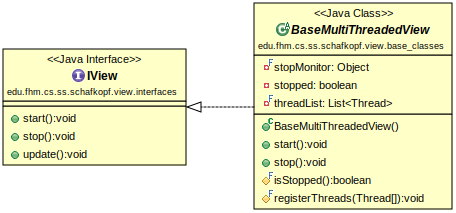
\includegraphics[width=0.9\textwidth]{./pictures/uml/class_diagram/uml_class_baseview.pdf}
	\caption[Anwendung/View -- Klassendiagramm Base Multithreaded View]{Klassendiagramm Base Multithreaded View} \label{fig:view_basemultithreaded}
\end{center}
\end{figure}

Von ihr werden folgende Methoden angeboten:
\begin{itemize}
	\item \textbf{\texttt{registerThreads(Thread...)}} registriert einen oder mehrere Threads und speichert sie in einer Liste. Diese können für Darstellung, Interaktion oder anderes zuständig sein.
Registrierte Threads dürfen noch nicht gestartet sein.
	\item \textbf{\texttt{start()}} startet alle registrierten Threads durch Aufruf von \textbf{\texttt{Thread.start()}}.
	\item \textbf{\texttt{stop()}} unterbricht jeden Thread in der Liste über \textbf{\texttt{Thread.interrupt()}} und setzt das Flag \textbf{\texttt{stopped}} auf true.
	\item \textbf{\texttt{isStopped()}} Bei einer Unterbrechung können Threads über diese Methode auf das Flag zugreifen und sich, sollte die Unterbrechung durch \textbf{\texttt{stop()}} hervorgerufen worden sein, beenden.
\end{itemize}\bigskip

Die typische Implementierung eines registrierten Threads sollte so aussehen:\bigskip

\begin{lstlisting}[{language=JAVA, label=lst:java_basemultithreadedview, caption={[Anwendung -- Typische Thread-Implementierung]{BaseMultiThreadedView -- typische Thread-Implementierung}}}]
private class DoSomethingThread extends Thread {
	@Override
	public void run() {
		// check flag, if set, this thread will terminate
		while (!isStopped()) {
			try {
				// do something, maybe wait() if nothing to do
			} catch (InterruptedException e) {
				// check flag
				if(isStopped()) {
					// interrupt caused by stop -> ok
				} else {
					// interrupt not caused by stop -> not ok
					// do interrupt handling
				}
			}
		}
	}
}
\end{lstlisting}

\clearpage

%% Beschreiben der Playerviews
\subsection{Playerviews} \label{sse:anwendung_views_player}
Die Playerviews werden unterteilt in zwei Klassen, die interaktiven und die autonomen Spieler. Das Klassendiagramm veranschaulicht den Zusammenhang. Der Üb\-er\-sicht\-lich\-keit halber sind Methoden und die Attribute bereits vorgestellter oder konkreter Klassen nicht dargestellt.

\begin{figure}[H]
\begin{center}
    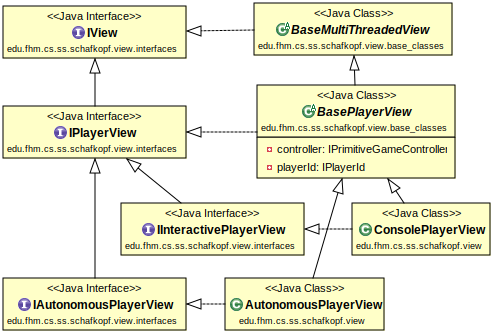
\includegraphics[width=1.0\textwidth]{./pictures/uml/class_diagram/uml_class_playerviews.pdf}
	\caption[Anwendung/View -- Struktur der Playerviews]{Struktur der Playerviews} \label{fig:views_player}
\end{center}
\end{figure}

Den konkreten Spielerklassen \textbf{\texttt{ConsolePlayerView}} und \textbf{\texttt{Au\-to\-no\-mous\-Pla\-yer\-View}} stehen die vererbten Methoden der bereits erwähnten \textbf{\texttt{Base\-Multi\-Threaded\-View}} und \textbf{\texttt{Ba\-se\-Pla\-yer\-View}} zur Verfügung.

\textbf{\texttt{IPlayerView}} definiert Zugriffsmethoden auf Id und Controller, sowie die \textbf{\texttt{update\-Game\-Data(IRes\-tric\-ted\-Pla\-yer\-Utils)}}-Methode, welche vom Controller aufgerufen wird, \newline 
wenn ein Zug auf den Spieldaten ausgeführt wurde. Der Parameter ist ein Utility-Wrapper auf einer eingeschränkten Kopie der aktuellen Spieldaten.

\textbf{\texttt{BasePlayerView}} enthält mit \textbf{\texttt{controller : IPrimitiveGameController}} den zu\-stän\-di\-gen Gamecontroller und kümmert sich im Konstruktor darum, den Spieler dort anzumelden (\autoref{sse:anwendung_controller_game}). \textbf{\texttt{playerId : IPlayerId}} wird benötigt, um sich beim Controller zu identifizieren und bei der Anmeldung von diesem gesetzt.

Die Interfaces \textbf{\texttt{IInteractivePlayerView}} und \textbf{\texttt{IAutonomoudPlayerView}} dienen\\ haupt\-säch\-lich der Kategorisierung der Spieler. \textbf{\texttt{IInteractiveView}} bietet allerdings noch Zugriffsmethoden auf die \acs{ki} (\autoref{se:anwendung_KI}).

%% Beschreiben der Console Player View
\subsubsection{Console Playerview} \label{ssse:anwendung_views_console_player}
Der Konsolenspieler ist eine einfache, interaktive View mit Darstellung. Die Darstellung der Spieldaten und das entgegennehmen von Benutzerinteraktionen laufen über die Konsole. Benutzerinteraktionen werden an \textbf{\texttt{IPrimitiveGameController}} weitergeleitet.
Wenn ein Aufruf von \textbf{\texttt{updateGameData(IRestrictedGameData)}} erfolgt, werden die erhaltenen Spieldaten in einen Puffer eingespeist. Ein für die Darstellung zuständiger Thread verbraucht die Daten aus dem Puffer. Somit ist gewährleistet, dass jede Änderung einmal dargestellt wird, auch wenn die Spieldaten-Aktualisierungen schneller erfolgen als der Darstellungs-Thread sie bearbeiten kann. Dabei muss zudem nur der Zugriff auf den Puffer synchronisiert werden und nicht die ganze Darstellung, was deutlich weniger Zeit kostet.\newline
Um Interaktionen des Benutzers entgegen zu nehmen, gibt es einen "'Consumer-Thread"' und einen "'Producer-Thread"'. Der Producer interpretiert Konsoleneingaben des Benutzers und generiert daraus passende Aktionen. Wenn eine Aktion generiert wurde, benachrichtigt er den Consumer.\newline
Dieser interagiert nun mit dem Controller und schickt ihm die Aktion zur Ausführung. Falls sie nicht erlaubt war, gibt er die Ursache aus.\newline
Da die Ausarbeitung der \acs{ui} keines der Hauptthemen dieser Bachelorarbeit war, wurden keine weiteren, interaktiven Views programmiert.
%% Beschreiben der AI Player View
\subsubsection{Autonomous Playerview} \label{ssse:anwendung_views_ai_player}
Der \acs{ki}-Spieler ist eine autonome View ohne Darstellung. Die Pufferung der Spieldaten erfolgt wie in \autoref{ssse:anwendung_views_console_player}. Jeder autonome Spieler enthält eine \acs{ki} (\autoref{se:anwendung_KI}), mit deren Hilfe er seine Aktionen generiert.\newline
Ein Thread ist für diese Generierung zuständig und arbeitet den Puffer mit den Spieldaten ab. Dafür wird mit \textbf{\texttt{IRes\-tric\-ted\-Pla\-yer\-Utils.\-is\-Ex\-pec\-ted\-To\-Act()}} überprüft, ob man aktiv werden muss und anschließend, abhängig vom aktuellen Spielzustand, die passende Methode der \acs{ki} aufgerufen, um eine Aktion zu erstellen. Diese wird dann an den \textbf{\texttt{IPrimitiveGameController}} weitergeleitet.\newline
Das Verhalten des \acs{ki}-Spielers wird vollständig durch seine \acs{ki} definiert. Er selbst ist sozusagen nur die ausführende Einheit. Besonders zu achten ist auf eine korrekte Funktionsweise der \acs{ki}. Sollte sie falsche, nicht erlaubte Züge berechnen, wird der Spieler nicht korrekt reagieren können und das Spiel zum Stillstand kommen da der Gamecontroller diese abweist.

%% Beschreiben der Settingsview
\subsection{Settingsview} \label{sse:anwendung_views_settings}
Die Settingsview ist ebenfalls eine Konsolenview, stellt \textbf{\texttt{IGameSettings}} dar und bietet ein Menü an, das Interaktionen zur Anpassung oder zum Speichern der Settings an den Controller weiterleitet. Die Weiterleitung erfolgt an \textbf{\texttt{IPrimitiveSettingsController}}. 
Bei einer erfolgreichen Änderung der Einstellungen ruft der Controller die \textbf{\texttt{update()}} Methode auf, wodurch die Darstellung der aktualisierten Settings in Gang gesetzt wird.\newline
Interaktionsmenü und Darstellung laufen in separaten Threads. Die Settingsview erbt daher ebenfalls von \textbf{\texttt{BaseMultiThreadeView}}.

%% Beschreiben der Startview
\subsection{Startview} \label{sse:anwendung_views_start}
Die Startview ist eine View ohne eigene Daten. Sie ist der Einstiegspunkt der Anwendung und bietet ein Menü zum Starten der \textbf{\texttt{SettingsView}} oder eines neuen Spiels, sowie zum Laden und Weiterspielen eines unterbrochenen Spiels. Zuständig für das Durchführen der Interaktionen ist der \textbf{\texttt{IPrimitiveStartController}}. Um einheitliche Views zu haben und die zur Verfügung gestellten Methoden nutzen zu können, erbt die Klasse von \textbf{\texttt{BaseMultithreadedView}}. Da es keine darzustellenden Daten gibt, bleibt \textbf{\texttt{update()}} leer.

\clearpage

%% Beschreiben der Controllerklassen
\section{Die Controller} \label{se:anwendung_controller}
Die Controller sind das Bindeglied zwischen View und Model Klassen. 
Sie bieten den Views Möglichkeiten, mit dem Model zu interagieren und informieren sie über durchgeführte Änderungen. Alle Controller haben Grundfunktionalitäten, die durch das Interface \textbf{\texttt{IController}} vorgegeben und durch die abstrakte Basisklasse \textbf{\texttt{BaseController}} implementiert sind.
Folgendes Diagramm stellt die Klassenstruktur am Beispiel des Gamecontrollers dar. Für die anderen Controller sind die Abhängigkeiten analog. Attribute werden, bis auf den in diesem Abschnitt erklärten \textbf{\texttt{BaseController}}, nicht dargestellt.

\begin{figure}[H]
\begin{center}
    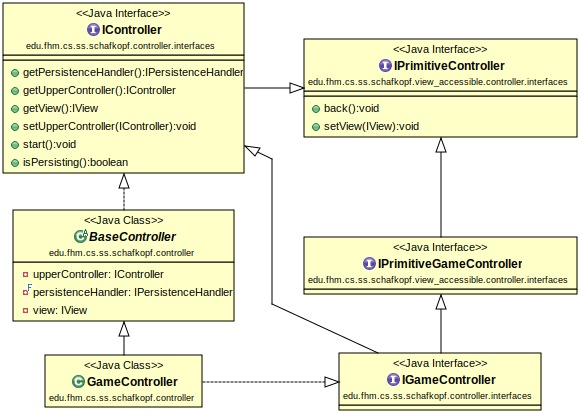
\includegraphics[width=1.0\textwidth]{./pictures/uml/class_diagram/uml_class_controller.pdf}
	\caption[Anwendung/Controller -- Struktur der Controller]{Struktur der Controller} \label{fig:controller_base}
\end{center}
\end{figure}

\textbf{\texttt{IPrimitiveController}} definiert die Schnittstelle, die Views zur Verfügung steht.
\begin{itemize}
	\item \textbf{\texttt{back()}} beendet alle Views des Controllers und navigiert über Aufruf von dessen \textbf{\texttt{start()}}-Methode zum vorherigen Controllers zurück.
	\item \textbf{\texttt{setView()}} wird verwendet um dem Controller eine View zuzuweisen. In der Regel setzen sich die Views bei ihrer Initialisierung selbst.
\end{itemize}\bigskip

Das \textbf{\texttt{IController}} Interface erweitert die Liste der Methoden um solche, die für das Erstellen und Starten eines Controllers nötig sind. Es steht nur anderen Controllern zur Verfügung.
\begin{itemize}
	\item \textbf{\texttt{getPersistenceHandler()}} und \textbf{\texttt{isPersisting()}} geben Information über die zu Grunde liegende Persistenzschicht. Ist ein \textbf{\texttt{IPersistenceHandler}} gesetzt, so hat der Controller die Möglichkeit, über diesen die Anwendungsdaten zu laden und zu speichern. Durch Aufruf von \textbf{\texttt{isPersisting()}} erfährt man, ob der Controller diese Möglichkeit auch nutzen soll. Sollte kein \textbf{\texttt{IPersistenceHandler}} zur Verfügung stehen, geben die Methoden  \textbf{\texttt{null}} bzw. \textbf{\texttt{false}} zurück.
	\item \textbf{\texttt{getView()}} liefert die View des Controllers zurück.
	\item \textbf{\texttt{getUpperController()}} und \textbf{\texttt{setUpperController(IController)}} ermöglichen es, einen Controller zu definieren, zu dem bei Aufruf von \textbf{\texttt{back()}} zurück navigiert wird.
	\item \textbf{\texttt{start()}} startet alle mit dem Controller zusammenhängenden Views.
\end{itemize}\bigskip

\textbf{\texttt{BaseController}} ist eine abstrakte Klasse und setzt oben erwähnte Grundfunktionalität um. Abgeleitete Controller müssen sich somit nur noch um die Kommunikation mit den Views und das Manipulieren der Anwendungsdaten kümmern.


%% Beschreiben des Gamecontrollers
\subsection{Gamecontroller} \label{sse:anwendung_controller_game}
Der Gamecontroller erbt zwar von \textbf{\texttt{BaseController}}, es werden jedoch einige der ererbten Methoden angepasst, da es mehrere Views gibt, mit denen eine Kommunikation stattfindet. Die Methoden \textbf{\texttt{start()}} und \textbf{\texttt{stop()}} werden überschrieben, so dass sie statt nur einer View, alle starten, bzw. terminieren. Er übernimmt außerdem die Aufgabe, bei Änderungen an den Spieldaten, alle angemeldeten Views mit einer personalisierten Kopie dieser zu, versorgen.

\textbf{\texttt{IPrimitiveGameController}} steht den Playerviews zur Verfügung, um mit dem Controller zu kommunizieren.
\begin{itemize}
	\item \textbf{\texttt{handleGameAction(IAction)}} nimmt eine Aktion des Spielers engegen, validiert diese und -- erfolgreiche Validierung vorausgesetzt -- führt sie auf den Spieldaten aus. Im Anschluss erhalten alle Spieler ein Update der aktualisierten Spieldaten. Die Methode liefert einen \textbf{\texttt{ActionValidationCode}} (\autoref{sse:anwendung_model_enums}) zurück, dem Spieler entnehmen können was mit ihrer Aktion passiert ist.
	\item \textbf{\texttt{subscribePlayer(IPlayerView)}} ermöglicht es den Playerviews, sich beim Controller zu registrieren. Die Registrierung ist nur bis vier Spieler möglich, da dies die maximale Anzahl an Spielern in Schafkopf ist. Weitere Aufrufe werden abgewiesen. Eine View, die erfolgreich registriert wurde, erhält vom Controller ihre \textbf{\texttt{IPlayerId}} gesetzt. Über diese wird in \textbf{\texttt{handleGameAction(IAction)}} der Spieler identifiziert.
\end{itemize}\bigskip

\textbf{\texttt{IGameController}} erweitert die Liste der Methoden nun um solche, auf die Views keinen Zugriff erhalten.
\begin{itemize}
	\item \textbf{\texttt{getGameData()}} und \textbf{\texttt{setGameData(IGameData)}} geben direkten Zugriff auf die\newline Spieldaten.
	\item \textbf{\texttt{notifyPlayers()}} Durch Aufruf dieser Methode erhalten alle Playerviews eine auf sie angepasste, eingeschränkte Kopie der Spieldaten. Dies geschieht normalerweise nach einer erfolgreich ausgeführten Aktion. Es wird die Liste der registrierten Spieler durchlaufen und die \textbf{\texttt{updateGameData(IPri\-mi\-ti\-ve\-Pla\-yer\-Utils)}}-Methode eines jeden aufgerufen. 
\end{itemize}\bigskip

Die konkrete Klasse \textbf{\texttt{GameController}} muss die in den Interfaces beschriebenen Anforderungen nun umsetzten. Dazu erhält sie eine Reihe von eigenen Attributen.
\begin{itemize}
	\item \textbf{\texttt{originalGameData : IGameData}} ist die Originalreferenz auf die Spieldaten. Die Spieler dürfen auf keinen Fall Zugriff auf diese erlangen. Aktionen der Spieler werden auf diesen Spieldaten ausgeführt. Bei einer Änderung werden alle registrierten Spieler mit einer eingeschränkten Kopie des Originals vom Typ \textbf{\texttt{RestrictedGameData}} versorgt. Aus der erstellten Kopie sind alle für den jeweiligen Spieler unzugänglichen Informationen komplett entfernt.
	\item \textbf{\texttt{nextSubscriberPosition : PlayerPosition}} Die Position, die dem nächsten sich registrierenden Spieler zugewiesen wird. 
	\item \textbf{\texttt{started : boolean}} wird in \textbf{\texttt{start()}} auf \textbf{\texttt{true}} und in \textbf{\texttt{back()}} auf \textbf{\texttt{false}} gesetzt. Sollte aus irgendeinem Grund eine View bereits aktiv sein und eine Aktion einreichen, während der Controller nicht gestartet wurde, wird diese abgewiesen. Spieler werden auch erst über Änderungen benachrichtigt, wenn dieses Flag gesetzt ist.
	\item \textbf{\texttt{playerViews : Map{\textless}IPlayerId, IPlayerView{\textgreater}}} Hier werden die Spieler, indiziert nach ihrer Spieler-ID, gespeichert. So kann, durch Vergleich mit gespeicherten IDs, bei Eingang einer Aktion recht komfortabel überprüft werden, ob der Spieler auf dem aktuellen Spiel angemeldet ist. Seine View kann dann direkt über die in der Aktion enthaltene ID indiziert werden.
\end{itemize}\bigskip

Die Methoden des \textbf{\texttt{GameController}}s sind threadsicher. Die kritischen Abschnitte sind alle über eigene Synchronisationsobjekte synchronisiert. (\autoref{ssse:grundlagen_java_threading})

\begin{itemize}
	\item Umsetzung von \textbf{\texttt{handleGameAction(IAction)}}:\newline
Da die Logik der Validierung und Ausführung von Aktionen in den Aktionsklassen steckt,  ist diese Methode recht kurz. Vor Validierung der Aktion wird die Spieler-ID überprüft und ob der Controller gestartet ist. Im Anschluss wird, synchronisiert über den Spieldaten, die Aktion validiert und bei Erfolg ausgeführt. Über ausgeführte Aktionen und dadurch geänderte Spieldaten werden die Spieler über \textbf{\texttt{notifyPlayers()}} benachrichtigt. Das Spiel wird nach jedem Zug persistiert, so dass es bei einer Unterbrechung, vom letzten Stand aus, fortgeführt werden kann.
	\item Umsetzung von \textbf{\texttt{subscribePlayer(IPlayerView)}}:\newline
Ein Spieler kann sich sowohl bei einem fortgeführten Spiel anmelden, als auch bei einem neuen Spiel. Ein registrierter Spieler wird bei Fortführen auf vorhandene Spielerdaten gemappt, bei Neustart werden neue Daten für ihn angelegt.
Die Spieler-ID wird in dieser Methode berechnet und gesetzt. Nach einer erfolgreichen Anmeldung wird \textbf{\texttt{nextSubscriberPosition}} inkrementiert.
\end{itemize}


%% Beschreiben des Startcontrollers
\subsection{Startcontroller} \label{sse:anwendung_controller_start}
Die Klasse \textbf{\texttt{StartController}} erbt von \textbf{\texttt{BaseController}} und bietet über die Schnittstelle \textbf{\texttt{IPrimitiveStartController}} folgende Interaktionsmöglichkeiten für die Views:

\begin{itemize}
	\item \textbf{\texttt{changeSettings()}} erstellt alle nötigen Komponenten für die Einstellungsansicht und startet diese im Anschluss.
	\item \textbf{\texttt{newGame()}} erstellt einen Gamecontroller mit neuen Spieldaten und den dazugehörigen Views, und startet diesen. Es beginnt ein neues Spiel eines Konsolenspielers gegen drei \acs{ki}-Spieler.
	\item \textbf{\texttt{resumeGame()}} lädt, falls vorhanden, über die Persistenzschicht gespeicherte Spieldaten und startet mit diesen ein Spiel. Falls keine Spieldaten vorhanden sind, kehrt die Methode mit dem Rückgabewert \textbf{\texttt{false}} zurück.
\end{itemize}

Durch Setzen des Startcontrollers als \textbf{\texttt{upperController}} der gestarteten Controller, kön\-nen diese zurück navigieren. Diese Klasse ist kein typischer Controller, da es keine Anwendungsdaten gibt, auf denen er arbeitet. Er kann als Einstiegspunkt der Anwendung gesehen werden und bietet Methoden, um die verschiedenen Ansichten des Prototypen zu starten.

%% Beschreiben des Settingscontrollers
\subsection{Settingscontroller} \label{sse:anwendung_controller_settings}
Der \textbf{\texttt{SettingsController}} erbt ebenfalls von \textbf{\texttt{BaseController}}. Falls sich die Einstellungen ändern, benachrichtigt er seine View über Aufruf von deren \textbf{\texttt{update()}}-Methode.

In \textbf{\texttt{IPri\-mi\-tive\-Set\-tings\-Con\-trol\-ler}} wird eine Methode für die Änderung von jedem Element der \textbf{\texttt{GameSettings}} definiert.
\begin{itemize}
	\item \textbf{\texttt{changeBasicCharge(int)}} Ändern der Zähleinheit.
	\item \textbf{\texttt{changePlayerName(PlayerPosition)}} ändert den Spielernamen an gegebener Position.
	\item \textbf{\texttt{changeSoloMultiplier(int)}} Ändern des Multiplikators für den Grundtarif eines Solospiels.
	\item \textbf{\texttt{changeStartMoney(int)}} Hier kann das Startgeld der Spieler angepasst werden.
		\item \textbf{\texttt{saveSettings()}} speichert die Einstellungen über die Persistenzschicht.
\end{itemize}\bigskip

\textbf{\texttt{ISettingsController}} gibt zusätzlich direkten Zugriff auf das Settingsobjekt. Der Controller übernimmt die Validierung der erhaltenen Änderungswünsche, so werden zum Beispiel leere Namen zurückgewiesen.

\clearpage

%% Beschreiben der Spielactions Klassen
\subsection{Spieleraktionen} \label{sse:anwendung_controller_game_actions}
Die Spieleraktionen kapseln die Logik der Validierung und Ausführung von Zügen auf den Spieldaten. Sie haben Zugriff auf \textbf{\texttt{IFullAccesGameUtils}} und können somit die gesamte Utility Funktionalität verwenden. Dadurch wird der Code in den Aktionsklassen übersichtlicher und gemeinsame Funktionalität muss nicht mehrfach programmiert werden. Alle Aktionen implementieren die Schnittstelle \textbf{\texttt{IAction}}. Der Gamecontroller kann über diese erhaltene Aktionen ausführen und validieren, ohne genau wissen zu müssen um welche es sich handelt. 

Die Klassenstruktur wird beispielhaft, anhand des Diagramms, für die konkrete Klasse
\textbf{\texttt{ChooseGameAction}} erläutert.

\begin{figure}[H]
\begin{center}
    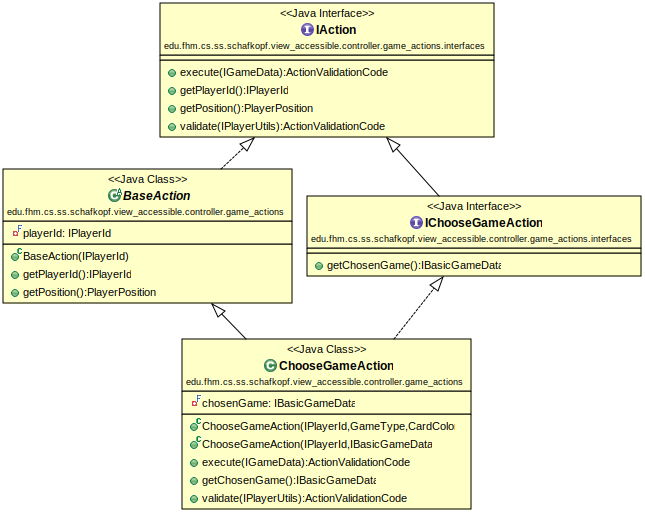
\includegraphics[width=1.0\textwidth]{./pictures/uml/class_diagram/uml_class_actions.pdf}
	\caption[Anwendung/Aktionen -- Struktur der Aktionen]{Struktur der Aktionen} \label{fig:controller_actions}
\end{center}
\end{figure}

Die Playerviews haben Zugriff auf alle Aktions Schnittstellen und konkreten Klassen. So können sie selbst eine Aktion instanziieren und diese zur weiteren Ausführung an den  Gamecontroller übergeben. Da Views keinen Zugriff auf die beiden Interfaces \textbf{\texttt{IGa\-me\-Da\-ta}} und \textbf{\texttt{IPlayerUtils}} haben, ist gewährleistet, dass sie die Aktionen nicht selbst aus\-füh\-ren oder validieren kön\-nen. Diese Methoden benötigen erwähnte Schnittstellen als Parameter.\newline
Das wird nicht benötigt, da die Views über \textbf{\texttt{IRestrictedPlayerUtils}} überprüfen kön\-nen, ob eine gewünschte Aktion erlaubt ist oder nicht. Bei nicht erlaubten Aktionen erhalten sie zudem bei versuchter Ausführung über \textbf{\texttt{handleGameAction(IAction)}} des Controllers, genauere Informationen über den Grund.

\textbf{\texttt{IAction}} definiert von allen Aktionen zu implementierende Methoden:
\begin{itemize}
	\item \textbf{\texttt{execute(IGameData)}} führt die Aktion auf den Spieldaten aus. Alle Änderungen, die durch die Aktion nötig sind, müssen hier korrekt erfolgen. Die Aktion ist selbst dafür zuständig, dass die Spieldaten konsistent bleiben. Es wird vorausgesetzt, dass nur valide Aktionen auch ausgeführt werden. Dafür bietet sich eine Überprüfung der Aktion auf den Spieldaten mittels \textbf{\texttt{va\-li\-date(IPla\-yer\-Utils)}} an. Es wird ein \textbf{\texttt{ActionValidationCode}} (\autoref{sse:anwendung_model_enums}) zu\-rück\-ge\-ge\-ben, der bei fehlgeschlagener Validierung den Fehler beschreibt und bei gültiger Validierung die Ausführung der Aktion.
	\item \textbf{\texttt{validate(IPlayerUtils)}} validiert die Aktion auf den Spieldaten der Utilities des Parameters. Der zurückgegebene \textbf{\texttt{ActionValidationCode}} (\autoref{sse:anwendung_model_enums}) beschreibt das Ergebnis der Validierung. Für die Validierung wird keine \textbf{\texttt{Full\-Ac\-ces\-Ga\-me\-Ut\-ils}} Instanz gebraucht, da keine Manipulationen auf den Daten durchgeführt werden sollen.
	\item \textbf{\texttt{getId()}} liefert die \textbf{\texttt{IPlayerId}} des Spielers, der die Aktion erstellt hat zurück. Diese wird im Konstruktor der Aktionen gesetzt.
	\item \textbf{\texttt{getPosition()}} liefert die Position der ID der Aktion zurück. 
\end{itemize}\bigskip

Da jede Aktion eine \textbf{\texttt{PlayerId}} besitzt, wird der Zugriff auf diese in eine abstrakte Basisklasse \textbf{\texttt{BaseAction}} ausgelagert. Die Bedeutung der Methoden können der Beschreibung der \textbf{\texttt{IAction}} Schnittstelle entnommen werden.

Das spezifische Interface, hier \textbf{\texttt{IChooseGameData}}, definiert den Zugriff auf die für die Aktion relevanten Datenelemente. Im Beispiel ist das:

\begin{itemize}
	\item \textbf{\texttt{getChosenGame()}} liefert das Spiel, das der Spieler mit der Aktion gerne anmelden würde.
\end{itemize}\bigskip

Die konkrete Aktion, hier \textbf{\texttt{ChooseGameAction}}, erbt von \textbf{\texttt{BaseAction}} und realisiert das spezifische Interface (\textbf{\texttt{IChooseGameData}}). Die Aktion muss sich um die Spieler ID nicht mehr kümmern. Im Konstruktor werden die Datenelemente festgelegt. Validierung und Ausführung muss hier in der konkreten Klasse implementiert werden. Die Umsetzungen für das Beispiel sind:
\begin{itemize}
	\item \textbf{\texttt{execute(IGameData)}}:\newline
 Zuerst wird wird ein \textbf{\texttt{IFullAccessUtils}}-Objekt erstellt, mit dem im Folgenden gearbeitet wird.
Dann wird die Aktion mit \textbf{\texttt{validate(IPlayerUtils)}} validiert. Ist die Validierung nicht erfolgreich, wird der Fehlercode direkt zurück gegeben, sonst fortgefahren.
Das angemeldete Spiel muss jetzt in den Spielerdaten (\textbf{\texttt{chosenGame}}) gespeichert und \textbf{\texttt{playerOnTurnPosition}} inkrementiert werden. Falls der gewählte Spieltyp das aktuelle Spiel dominiert, wird es -- genauso wie die \textbf{\texttt{le\-ad\-Pla\-yer\-Po\-si\-ti\-on}} in den Spieldaten -- überschrieben. \newline
Haben alle Spieler ihr Spiel ausgewählt, was mit \textbf{\texttt{Utils.haveAllPlayersChosen()}} überprüft wird, muss der Spielstatus auf \textbf{\texttt{PLAY}} und die Rundennummer auf 0 gesetzt werden.
Außer alle Spieler haben gepasst, dann ist das Spiel zu Ende und die \textbf{\texttt{Utils.endGameManipulations()}} werden ausgeführt.
	\item \textbf{\texttt{validate(IPlayerUtils)}}:\newline
Diese Implementierung ist sehr kurz und verwendet \textbf{\texttt{Utils.get\-Cho\-ose\-Ga\-me\-Va\-li\-da\-ti\-on\-Co\-de}} für die Validierung. Der erhaltene \textbf{\texttt{ActionValidationCode}} wird zurückgegeben.
\end{itemize}\bigskip

Die beschriebenen Abhängigkeiten und die Vorgehensweise der Implementierung finden sich in allen Aktionen wieder, weshalb diese der Vollständigkeit halber zwar noch aufgeführt, jedoch nicht mehr eingehend beschrieben werden.

\textbf{\texttt{GetCardsAction}} gibt dem ausführenden Spieler Karten, solange seine Hand nicht voll ist und das Spiel sich im Zustand \textbf{\texttt{GET{\_}RAISE}} befindet.

\textbf{\texttt{PlayCardAction}} spielt die Karte, mit der die Aktion erstellt wird für den ausführenden Spieler. Die Karte wird aus der Hand des Spielers entfernt und alle nach einem Zug nötigen Änderungen an den Spieldaten durchgeführt. Die Karte muss sich in der Hand des Spielers befinden und sonstige Bedingungen für das Spielen der Karte erfüllt sein.

\textbf{\texttt{RaiseAction}} lässt den Spieler legen. Die Tarifdaten werden entsprechend angepasst. Gelegt werden darf nur einmal, wenn sich das Spiel im richtigen Zustand befindet und der Spieler noch nicht alle Karten auf der Hand hat.

\textbf{\texttt{StartNextGameAction}} darf zu jedem Zeitpunkt des Spiels ausgeführt werden, aber nur einmal pro Spieler. Damit signalisiert dieser, dass er das aktuelle Spiel nicht mehr weiterspielen, sondern gerne das Nächste beginnen würde. Spätestens wenn sich das Spiel im Status \textbf{\texttt{FINISHED}} befindet, sollten von allen Spielern diese Aktionen eingehen, da sonst das Nächste nicht gestartet wird.

\textbf{\texttt{StrikeAction}} und \textbf{\texttt{StrikeBackAction}} lassen den Spieler stoßen bzw. Retour geben, wenn die Voraussetzungen dafür erfüllt sind. Es ist ein Wahrheitswert als Attribut enthalten. Dieser ist \textbf{\texttt{true}}, wenn der ausführende Spieler stoßen möchte, sonst \textbf{\texttt{false}}. Die Aktionen werden auch ausgeführt, wenn der Spieler nicht an der Reihe ist. Sollte sich das Spiel im Zustand \textbf{\texttt{STRIKE}} befinden, müssen alle Spieler, für die die Voraussetzungen für die Aktion erfüllt sind, diese auch an den Controller weiterleiten.
%%%%%%%%%%%%%%%%%%%%%%%%%%%%%%%%%%%%%%%%%%%%%%%%%%%%%%%%%%%%%%%%%%%%%%%%
%%%%%%%%%%%%%%%%%%%%%%  KORREKTUR 2 bis hier  %%%%%%%%%%%%%%%%%%%%%%%%%%
%%%%%%%%%%%%%%%%%%%%%%%%%%%%%%%%%%%%%%%%%%%%%%%%%%%%%%%%%%%%%%%%%%%%%%%%
%% Wie funktioniert die Navigation zwischen den Views
\section{Navigation} \label{se:anwendung_navigation}
Im Prototypen ist eine einfache Navigation definiert, die über die Controller funktioniert. Jeder Controller wird im Konstruktor mit eine Parameter \textbf{\texttt{upperController}} vom Typ \textbf{\texttt{IController}} initialisiert.
Über die \textbf{\texttt{IPrimitiveController}} Schnittstelle wird allen Views eine Methode \textbf{\texttt{back()}} angeboten. Diese beendet alle Views des Controllers und ruft anschließend die \textbf{\texttt{start()}} Methode des \textbf{\texttt{upperController}}s auf. Dadurch wird die vorherige Ansicht wieder hergestellt.\newline
Wenn in die Anwendung hinein navigiert wird, sollten die tiefer liegenden Controller immer mit dem Controller einer Ebene darüber initialisiert werden. Recht gut zu erkennen ist das an der Implementierung von \textbf{\texttt{StartController}}.
Das Codebeispiel zeigt die Verwendung anhand der Navigation in die Settingsview und zurück.\bigskip

\begin{lstlisting}[{language=JAVA, label=lst:app_navigation, caption={[Anwendung -- Navigationsbeispiel]{Navigation am Beispiel Startview / Settingsview}}}]
/**
 * Navigate to the Settingsview. (StartController)
 */
public void changeSettings() {
	// stop the controllers view components
	getView().stop();
	// initialize the controller with "this" as the upperController
	final ISettingsController settingsController = new 												SettingsController(getPersistenceHandler(), this);
	// create the view
	new ConsoleSettingsView(settingsController);
	// start the controller
	settingsController.start();
}
/**
 * Navigate back to the upper controller. (SettingsController, 
 * implemented in BaseController)
 */
public void back() {
	// stop connected views
	if (this.view != null) {
		this.view.stop();
	}
	// start upper controller
	if (upperController != null) {
		upperController.start();
	}
}
\end{lstlisting}

%% Wie funktioniert die Persistenz
\section{Persistenz} \label{se:anwendung_persistenz}
Die Persistenzschicht der Anwendung wird über die Schnittstelle \textbf{\texttt{IPersistenceHandler}} beschrieben. Diese definiert Methoden, um Objekte zu laden und abzuspeichern.

\begin{itemize}
	\item \textbf{\texttt{load(String)}} lädt ein Objekt, der Parameter ist der Dateiname.
	\item \textbf{\texttt{persist(IPersistenceObject)}} speichert ein Persistenzobjekt. Dieses wird weiter unten erklärt. Es muss kein Dateiname angegeben werden, da jedes Persistenzobjekt diesen anbietet.
	\item \textbf{\texttt{persist(Object, String)}} speichert ein beliebiges Objekt unter gegebenem Dateinamen.
	\item \textbf{\texttt{setPrefix(String)}} und \textbf{\texttt{getPrefix()}} geben Zugriff auf das Prefix, das vor den Dateinamen aller abgespeicherten Objekte, angefügt wird.
\end{itemize}

Der Prototyp verwendet als konkrete Implementierung obiger Schnittstelle den \textbf{\texttt{XML\-Fi\-le\-Per\-sis\-ten\-ce\-Han\-dler}}. Dieser lädt und speichert unter Verwendung der in \autoref{ssse:grundlagen_java_xstream} vorgestellten Bibliothek, die Objekte als XML-Dateien im aktuellen Ordnerpfad der Anwendung.

Die Interfaces \textbf{\texttt{IPersistenceObject}} und \textbf{\texttt{IPersistableObject}} sind für den Fall, dass sich das Java-Objekt (\textbf{\texttt{IPersistableObject}}) von dem unterscheidet, das die Persistenzschicht konkret abspeichert (\textbf{\texttt{IPersistenceObject}}), gedacht. Die Schnittstellen umsetzende Klassen müssen jeweils eine Methode anbieten, um das \textbf{\texttt{IPer\-sis\-ta\-ble\-Ob\-ject}} in ein \textbf{\texttt{IPersistenceObject}} zu konvertieren oder umgekehrt.\newline
Der Dateiname eines \textbf{\texttt{IPersistenceObject}}s wird durch \textbf{\texttt{getFilename()}} zurück gegeben.\newline
Da im Prototypen direkt die Java-Objekte abgespeichert werden, implementieren persistierbare Daten beide Schnittstellen und geben bei Aufruf der Konvertierungsmethoden eine Referenz auf sich selbst zurück.

\clearpage

%% Wie funktioniert die KI
\section{KI} \label{se:anwendung_KI}
Die Entwicklung einer neuen \acs{ki} wird durch die im Prototypen festgelegte Struktur erleichtert. Abhängigkeiten zu anderen Programmteilen sind auf ein Minimum reduziert. Solange eine \acs{ki} die vorgegebene Schnittstelle implementiert, kann sie direkt in die Anwendung eingebunden werden.\newline
Es gibt zwei Kategorien, eine ist für Fragen zuständig, die unabhängig vom angemeldeten Spiel beantwortbar sind, die andere für solche, die man nur abhängig von diesem beantworten kann.\newline
Eine vollständige \acs{ki} sollte Fragen beider Kategorien beantworten können und deshalb beide Schnittstellen implementieren. Es bot sich an, in der vollständigen \acs{ki} die allgemeinen Fragen selbst zu implementieren und die spezialisierten Fragen an eine Instanz weiterzuleiten, die nur für diese zuständig ist. Die Logik bleibt so getrennt und der Code damit übersichtlicher. Durch diese Struktur vereinfacht sich auch der Start des nächsten Spiels für die \acs{ki}. Da die allgemeinen Fragen ja weiterhin beantwortet werden können, muss sie nur ihre spezialisierte \acs{ki} an das nächste Spiel anpassen.
Um diese Aktualisierung weitestgehend zu automatisieren wurde eine Basisklasse implementiert, die dafür zuständig ist.
Die Klassen und Methoden verwenden alle die englische Bezeichnung \acf{ai}.

\clearpage

Die Struktur wird am Beispiel des \textbf{\texttt{SimpleDeterministic\acs{ai}}}-Sets in folgendem Diagramm veranschaulicht. Da die Liste der Methoden und Attribute nicht allzu umfangreich ist und das Verständnis des Diagramms erleichtert, sind diese mit aufgeführt.

\begin{figure}[H]
\begin{center}
    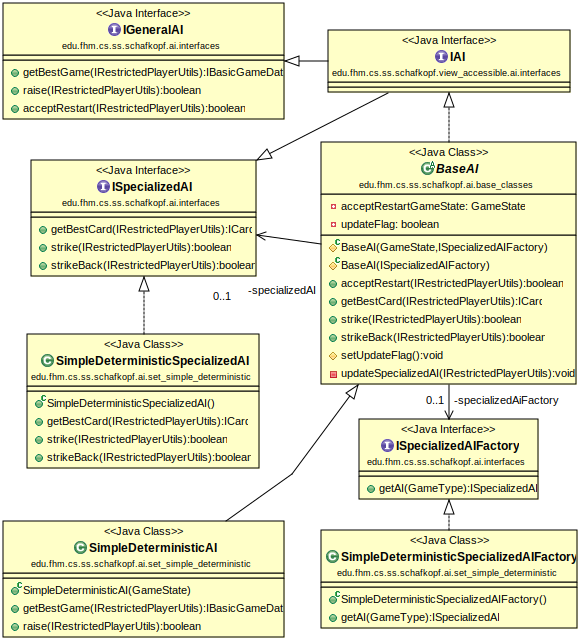
\includegraphics[width=1.0\textwidth]{./pictures/uml/class_diagram/uml_class_ai.pdf}
	\caption[Anwendung/\acs{ki} -- Struktur der \acs{ki} am Beispiel]{Struktur der \acs{ki}} \label{fig:ai}
\end{center}
\end{figure}

Zur Erklärung werden nun die Klassen und Interfaces, sowie deren Abhängigkeiten, der Reihe nach beschrieben. Alle Methodenaufrufe benötigen als Parameter eine Referenz auf \textbf{\texttt{IRestrictedPlayerUtils}}, aus dem sie die Spiel- und Spielerinformationen entnehmen können. Diese wird in den Auflistungen nicht aufgeführt.

Die beiden Interfaces \textbf{\texttt{IGeneral\acs{ai}}} und \textbf{\texttt{ISpecialized\acs{ai}}} stellen die beiden bereits er\-wähn\-ten Kategorien dar.

\textbf{\texttt{ISpecialized\acs{ai}}} ist abhängig von einem konkreten Spiel und muss entsprechend initialisiert werden. Eine \acs{ki}, die z.B. auf Sauspiel spezialisiert ist, wird nämlich für andere Spieltypen voraussichtlich falsche Antworten geben.
\begin{itemize}
	\item \textbf{\texttt{getBestCard(...)}} gibt dem Spieler die Karte zurück, die er am besten spielen sollte.
	\item \textbf{\texttt{strike(...)}} sagt dem Spieler, ob er stoßen und
	\item \textbf{\texttt{strikeback(...)}} ob er Retour geben sollte.
\end{itemize}\bigskip

\textbf{\texttt{IGeneral\acs{ai}}} ist die Schnittstelle für eine allgemeine \acs{ki} und beantwortet mit seinen Methoden alle von einem konkreten Spiel unabhängigen Fragen.
\begin{itemize}
	\item \textbf{\texttt{getBestGame(...)}} beantwortet die Frage nach dem Spiel, das sich am besten für die Hand des Spielers eignet.
	\item \textbf{\texttt{raise(...)}} sagt dem Spieler, ob er mit seinen Karten legen sollte.
	\item \textbf{\texttt{acceptRestart(...)}} gibt zurück, ob der Spieler den Start des nächsten Spiels akzeptieren sollte.
\end{itemize}\bigskip

\textbf{\texttt{I\acs{ai}}} erweitert die beiden obigen Interfaces, und bietet somit spezialisierte und allgemeine Methoden an.

\textbf{\texttt{ISpecialized\acs{ai}Factory}} ist die Schnittstelle für eine statische Factory-Klasse, sie liefert mit \textbf{\texttt{get\acs{ai}(GameType)}} eine auf den Spieltypen zugeschnittene, spezialisierte \acs{ki} zurück. Sie wird verwendet, um die spezialisierte \acs{ki} passend zu initialisieren.

Die abstrakte Klasse \textbf{\texttt{Base\acs{ai}}} implementiert die Grundfunktionalität. Sie kümmert sich um das Initialisieren der passenden spezialisierten \acs{ki} und gibt Antwort auf die Frage, ob der Start des nächsten Spiels akzeptiert werden soll. Um ihre Aufgaben erledigen zu können, muss sie im Konstruktor die benötigten Attribute geliefert bekommen.
\begin{itemize}
	\item \textbf{\texttt{acceptRestartGameState : gameState}} enthält den Spielstatus, bei dem \textbf{\texttt{ac\-cept\-Re\-start(...)}} mit \textbf{\texttt{true}} beantwortet wird. Sollte dieser Wert \textbf{\texttt{null}} sein, so wird der Neustart immer akzeptiert. Das nächste Spiel wird erst gestartet, wenn alle Spieler ihre Einwilligung gegeben haben.
	\item \textbf{\texttt{updateFlag : boolean}} Von diesem Flag ist abhängig, ob die spezialisierte \acs{ki} aktualisiert wird.
	\item \textbf{\texttt{specialized\acs{ai} : ISpecialized\acs{ai}}} An diese \acs{ki} werden alle ein spezielles Spiel betreffende Fragen weitergeleitet. Die Weiterleitung wird hier implementiert.
	\item \textbf{\texttt{specialized\acs{ai}Factory : ISpecialized\acs{ai}Factory}} wird zur Initialisierung der \textbf{\texttt{specialized\acs{ai}}} verwendet.
	\item \textbf{\texttt{acceptRestart(...)}} gibt zurück, ob ein Neustart akzeptiert wird.
	\item \textbf{\texttt{getBestCard(...)}} wird an \textbf{\texttt{specialized\acs{ai}}} weitergeleitet.
	\item \textbf{\texttt{strike(...)}} wird an \textbf{\texttt{specialized\acs{ai}}} weitergeleitet.
	\item \textbf{\texttt{strikeBack(...)}} wird an \textbf{\texttt{specialized\acs{ai}}} weitergeleitet.	
	\item \textbf{\texttt{setUpdateFlag()}} gibt ableitenden Klassen die Möglichkeit, zu signalisieren, dass \textbf{\texttt{specialized\acs{ai}}} nicht mehr aktuell ist.
	\item \textbf{\texttt{updateSpecialized\acs{ai}(...)}} wird jedesmal, bevor eine Methode an \textbf{\texttt{spe\-ci\-ali\-zed\-\acs{ai}}} weitergeleitet wird, aufgerufen. Sollte \textbf{\texttt{updateFlag}} gesetzt sein, wird diese vor der Weiterleitung über \textbf{\texttt{specialized\acs{ai}Factory}} aktualisiert und das Flag wieder auf \textbf{\texttt{false}} gesetzt.
\end{itemize}\bigskip

Die konkrete, allgemeine \acs{ki}-Klasse \textbf{\texttt{SimpleDeterministic\acs{ai}}} muss nun darauf achten, dass \textbf{\texttt{Base\acs{ai}}} mit der richtigen \textbf{\texttt{ISpecialized\acs{ai}Factory}} initialisiert wird. Das sollte im Konstruktor erledigt werden. Außerdem hat sie die Aufgabe, über \textbf{\texttt{setUpdateFlag()}}, dieser mitzuteilen, wann die Aktualisierung der spezialisierten \acs{ki} nötig ist. Es bietet sich an das in der \textbf{\texttt{getBestGame(...)}}-Methode zu tun, da diese bei jedem neuen Spiel einmal aufgerufen wird.\newline
Die allgemeinen Fragen, also nach dem besten Spiel und ob man legen sollte, müssen hier umgesetzt werden. Auf deren genaue Implementierung wird nicht näher eingegangen. Wie der Name aber bereits vermuten lässt, handelt die \acs{ki} einfach und deterministisch.

\textbf{\texttt{SimpleDeterministicSpecialized\acs{ai}}} muss sich um nichts anderes als die Implementierung der übrig bleibenden, spielabhängigen Methoden kümmern. Auf diese wird hier auch nicht näher eingegangen. Sie sind einfach gehalten und deterministisch.

\textbf{\texttt{SimpleDeterministicSpecialized\acs{ai}Factory}} gibt im konkreten Fall bei Aufruf ihrer Factory-Methode, immer eine neue Instanz der \textbf{\texttt{SimpleDeterministic\acs{ai}}} zurück. Normalerweise sollte eine auf jeden Spieltyp angepasste \acs{ki}-Version zurückgegeben werden.\bigskip

\clearpage

Mit Hilfe dieser Struktur ist es möglich, sehr komfortabel und ohne weitere Codeanpassungen, ein neues \acs{ki}-Set zu entwickeln. Für ein Set braucht man eine Factory, die die spezialisierten \acs{ki}s aus dem Set liefert, eine allgemeine \acs{ki}, welche von \textbf{\texttt{Base\acs{ai}}} erben sollte, sowie eine Menge von spezialisierten \acs{ki}s für die verschiedenen Spieltypen.

Im Prototypen gibt es drei Sets, das oben beschriebene und eines, das zufällige, aber erlaubte Züge macht. Das Dritte definiert nur die Grundstruktur eines Sets, das abhängig vom Spieltypen verschiedene spezialisierte \acs{ki}s verwendet und sollte nicht benutzt werden, da die Methodenrümpfe nicht implementiert sind. Aus diesem Grund ist letzteres als \textbf{\texttt{deprecated}} eingestuft.
\clearpage

%% Beschreibung der Testumgebung
\chapter{Die Testumgebung} \label{ch:testing}
Das Ergebnis des zweiten großen Schwerpunkts der Programmierung ist die Testumgebung. Mit ihr lässt sich die korrekte Funktionalität des Prototypen überprüfen und somit nachweisen, dass dieser wie vorgesehen arbeitet.\newline
Des Weiteren werden nachfolgende Änderungen am Prototypen, die einen unvorhergesehenen Programmablauf zur Folge haben detektiert. Sollte dieser ausdrücklich erwünscht sein, muss der Entwickler bewusst den entsprechenden Test modifizieren. Damit wird sichergestellt, dass durch Änderungen nicht aus Versehen die Funktionalität beeinträchtigt wird. Sollten \acs{ki}s unerlaubte Züge vorschlagen, erkennt der Custom Stresstest mit den \acs{ki}s den daraus folgenden Stillstand des Spiels. Ein auf deterministische \acs{ki}s spezialisierter Test erkennt, wenn diese sich bei gleichen Voraussetzungen unterschiedlich verhalten.

Die Testumgebung liegt im Quellordner \textbf{src\_test} und ist somit vom Code der Anwendung weitgehend abgekapselt.

Die Packagestruktur spiegelt die unterschiedlichen Aufgabenbereiche der Klassen wider.
\begin{itemize}
	 \item \textbf{.application} Hier liegt die Testanwendung.
	 \item \textbf{.controller} Der Testcontroller bietet die für die Testanwendung verfügbaren Methoden zum Starten der Tests.
 	 \item \textbf{.model} Alle Testdaten sind in diesem Package untergebracht.
 	 \item \textbf{.recording} enthält Klassen zum Starten und Aufzeichnen eines Testspiels.
 	 \item \textbf{.settings} Einstellungsoptionen für die Tests.
 	 \item \textbf{.formattingandvalidation} Utilityklassen für die Validierung von Spieldaten und Formatierung dieser für die Fehlerausgabe.
\end{itemize}

\clearpage

%% Ein Testfall, was wird gespeichert und warum
\section{Testdaten} \label{se:testing_data}
Es stellt sich die Frage, was alles gespeichert werden muss, um ein komplettes Spiel zu überprüfen. Da sich die Testfälle nach und nach entwickelt haben, sind auch die Anforderungen an die Testdaten mit der Zeit gewachsen. \newline
Die Klasse \textbf{\texttt{TestGameData}} ist die finale Datenklasse und enthält alle Daten, die für Untersuchung oder Ausgabe notwendig sind. Die implementierte Schnittstelle \textbf{\texttt{ITest\-Ga\-me\-Da\-ta}} definiert Methoden, um auf diese Daten zuzugreifen.

\begin{itemize}
	\item \textbf{\texttt{fileName : String}} Unter diesem Namen werden die Daten abgespeichert. 
	\item \textbf{\texttt{acceptRestartState : GameState}} Der Spielstatus, bei dem die für den Test verwendete \acs{ki} den Start des nächsten Spiels akzeptiert. Da der Wert nicht in den Spieldaten gespeichert ist, sondern in den \acs{ki}s, muss er separat aufgezeichnet werden.
	\item \textbf{\texttt{initialStack : List{\textless}ICard{\textgreater}}} Eine Kopie des Kartenstapels, mit dem das Spiel initialisiert wurde. Dieser könnte auch aus dem ersten Spielstand berechnet werden, da hier aber die erste Aktion bereits ausgeführt wurde, meist eine \textbf{\texttt{GetCardsAction}}, ist er nicht mehr vollständig.
	\item \textbf{\texttt{players : Map{\textless}Class{\textless}? extends IPlayerView{\textgreater}{\textgreater}}} enthält die Klassen der Pla\-yer\-vi\-ews, mit denen dieser Testfall erstellt wurde. 
	\item \textbf{\texttt{ais : Map{\textless}Class{\textless}? extends I\acs{ai}{\textgreater}{\textgreater}}} enthält die \acs{ki}-Klassen, mit denen die autonomen Playerviews initialisiert wurden. 
	\item \textbf{\texttt{gamesList : List{\textless}IGameData{\textgreater}}} Zu dieser Liste werden die Spielzustände eines Spiels der Reihe nach hinzugefügt. Somit kann in einem Testfall die komplette Spielentwicklung nachvollzogen werden.
	\item \textbf{\texttt{actionList : List{\textless}IActionData{\textgreater}}} Da die Spieldaten nur die ausgeführten Aktionen enthalten, es jedoch für Tests und Ausgabe von Interesse ist, alle Aktionen in der richtigen Reihenfolge ihrer Bearbeitung einzusehen, werden diese hier aufgelistet.
	\item \textbf{\texttt{deterministicActionList : List{\textless}IActionData{\textgreater}}} enthält alle de\-ter\-mi\-nis\-ti\-schen Aktionen. Aktionen wie \textbf{\texttt{StartNextGameAction}} sind nicht enthalten, da diese zu einem beliebigen Zeitpunkt eintreffen ausgeführt werden können.
	\item \textbf{\texttt{raiseActionList : List{\textless}IActionData{\textgreater}}} \textbf{\texttt{RaiseAction}} Der Zeitpunkt der Aus\-füh\-rung einer \textbf{\texttt{RaiseAction}} ist nicht relevant, sondern nur ob ein Spieler gelegt hat oder nicht. Deshalb werden diese hier in dieser Liste aufgeführt und im De\-ter\-mi\-nis\-mus\--Test nur überprüft, ob die jeweiligen Spieler im wiederholten Spiel ebenfalls gelegt haben. Eine \textbf{\texttt{RaiseAction}} wird demnach nicht in \textbf{\texttt{deterministicActionList}} aufgenommen.
\end{itemize}

\textbf{\texttt{acceptRestartState}}, \textbf{\texttt{initialStack}}, \textbf{\texttt{players}} und \textbf{\texttt{ais}} sind Daten, die benötigt werden, um den Testfall im Determinismus-Test unter gleichen Vorbedingungen nachzuspielen. Die anderen Attribute finden in den unterschiedlichen Validierungen des Spielablaufs sowie zur Ausgabe von Informationen Verwendung.\bigskip

\textbf{\texttt{TestValidationInfo}} ist eine weitere Datenklasse und sammelt alle Informationen, die bei der Ausführung und Validierung von Tests anfallen. Sie implementiert \textbf{\texttt{ITest\-Va\-li\-da\-ti\-on\-In\-fo}}, welche -- neben Zugriffsmethoden -- auch solche zum formatierten Anfügen von Testinformationen bietet. Auf die Zugriffsmethoden wird hier nicht eingegangen.
\begin{itemize}
	\item \textbf{\texttt{totalValidationCode : TestValidationCode}} Der Code, mit dem dieser Testfall abgeschlossen wurde. Jeder Fehler, der während des Tests auftritt, wird mit einem Code und der Fehlerbeschreibung an die Testinformationen angehängt. Sollte der neue Code von höherer Priorität sein als die von \textbf{\texttt{totalValidationCode}}, so wird er über\-nom\-men. So kann auf einen Blick eingesehen werden, ob Fehler aufgetreten und welcher Kategorie sie sind. Dieses Attribut wird mit \textbf{\texttt{SUCCESS}} initialisiert.
	\item \textbf{\texttt{furtherInformation : StringBuilder}} Ein interner \textbf{\texttt{StringBuilder}}, der verwendet wird, um Testinformationen formatiert anzufügen.
	\item \textbf{\texttt{testGameData : ITestGameData}} Die Test-Spieldaten sind optional, da nicht alle Tests auf Spieldaten ausgeführt werden. Diese sind der Vollständigkeit halber angehängt, um den Zusammenhang zwischen den Validierungsdaten und den Spieldaten herzustellen.
	\item \textbf{\texttt{appendInformation(TestValidationCode, String)}} hängt an \textbf{\texttt{fur\-ther\-In\-for\-ma\-ti\-on}} den gegebenen \textbf{\texttt{TestValidationCode}} und anschließend die mit dem zweiten Parameter übergebenen Informationen zum Fehler an. Sollte die Priorität des Codes höher sein als von \textbf{\texttt{totalValidationCode}}, so wird er übernommen. 
\end{itemize}\bigskip

Der Aufzählungstyp \textbf{\texttt{TestValidationCode}} definiert folgende Fehlercodes:
\begin{itemize}
	\item \textbf{\texttt{SUCCESS}} Priorität 0, der Test war erfolgreich. 
	\item \textbf{\texttt{WARNING}} Priorität 1, Warnung, wird zum Beispiel bei Nichtdeterminismus der \acs{ki}s gesetzt, da dies nicht zwingend ein Fehler ist.
	\item \textbf{\texttt{ERROR\_INVALID\_ACTION\_EXECUTION}} Priorität 2, es ist ein Fehler bei der Ausführung einer Aktion aufgetreten. Dies kann unerlaubte Ausführung auf dem aktuellen Spielzustand oder unerlaubte Manipulation durch die Aktion sein.
	\item \textbf{\texttt{ERROR\_NON\_CRITICAL\_INVALID\_STATE}} Priorität 3, die Spieldaten enthalten un\-gül\-ti\-ge Werte, die jedoch nicht kritisch sind. Das heißt es kommt in der Regel dadurch nicht zum Programmabsturz. Zum Beispiel, wenn das Spiel zu Ende, aber das Gewinnerteam nicht gesetzt ist.
	\item \textbf{\texttt{ERROR\_DEADLOCK}} Priorität 4, bei der Ausführung des Tests ist ein Deadlock aufgetreten. Das Spiel befand sich über längere Zeit im Stillstand und wurde abgebrochen.
	\item \textbf{\texttt{ERROR\_CRITICAL\_INVALID\_STATE}} Priorität 5, kritischer Fehler in den Spieldaten z.B. \textbf{\texttt{null}}-Werte. Durch kritische ungültige Daten kann es zu Ausnahmen während des Spielablaufs kommen.
	\item \textbf{\texttt{ERROR\_GENERAL}} Priorität 6, ein genereller Fehler beim Starten des Tests, kann durch Fehler beim Laden/Speichern der Testdaten, Tests die nichts mit dem Spielablauf zu tun haben, oder nicht in obige Kategorien einzuordnen sind, auftreten.
\end{itemize}

\clearpage

%% Ein Testfall, was wird gespeichert und warum
\section{Aufzeichnung der Testdaten} \label{se:testing_recording}
Für die Aufzeichnung der Testdaten bietet sich ein weiterer passiver Spieler an, der die vom \textbf{\texttt{GameController}} erhaltenen Informationen in die Datenklasse aus \autoref{se:testing_data} schreibt. Dieser wird im Folgenden "'Recorder"' genannt.\newline
Der \textbf{\texttt{GameController}} liefert allerdings nicht alle benötigten Informationen - nur eingeschränkte Spieldaten - und bietet außerdem keine Möglichkeit, einen zusätzlichen fünften Spieler anzumelden.\newline
Da für die Testumgebung der Anwendungscode nicht verändert werden soll, wurde ein neuer Controller geschrieben, der von \textbf{\texttt{GameController}} erbt und in dem die zusätzliche Funktionalität untergebracht ist.\newline
Der Recorder muss dann auch nicht mehr das \textbf{\texttt{IPlayer}}-Interface implementieren und konnte so freizügiger gestaltet werden.
 
%% Was macht der Game Recorder
\subsection{Gamerecorder} \label{sse:testing_observer}
\textbf{\texttt{GameRecorder}} implementiert \textbf{\texttt{IGameRecorder}} und ist die konkrete Umsetzung des Recorders. Er wird vom \textbf{\texttt{TestGameController}} (\autoref{sse:testing_controller_game}) mit Informationen versorgt, mit denen während des Spielverlaufs die Testdaten befüllt werden.\newline
Ist das Spiel zu Ende liefert er seinem Controller über \textbf{\texttt{test\-Fe\-ed\-back\-(ITest\-Va\-li\-da\-ti\-on\-In\-fo)}} die erstellten Daten. Der Recorder ist threadsicher, seine Update Methoden sind synchronisiert.
\begin{itemize}
	\item \textbf{\texttt{updateMonitor : Object}} Das Synchonisationsobjekt für eingehende Updates.
	\item \textbf{\texttt{finished : boolean}} signalisiert ein planmäßig zu Ende gespieltes Spiel.
	\item \textbf{\texttt{interactive : boolean}} Ist dieses Flag gesetzt, so ist der Deadlock-Timeout des Controllers außer Kraft gesetzt. Ein interaktiver Spieler hat unbeschränkt Zeit, seinen Zug zu machen.
	\item \textbf{\texttt{testGameData : ITestGameData}} Die Testdaten, die bei Updates mit den erhaltenen Daten befüllt werden.
	\item \textbf{\texttt{controller : ITestGameController}} Der Recorder kennt seinen Controller, er muss sich ja bei diesem rückmelden.
	\item \textbf{\texttt{validState : boolean}} signalisiert unzulässige Spieldaten, dieses Flag wird intern verwendet. Es wird gesetzt, wenn ein Fehler gefunden wurde. Dadurch wird dem Controller gleich das Feedback geschickt, ohne auf weitere Testdaten zu warten. Bei erhalt des Feedbacks bricht der Controller das laufende Spiel ab.
	\item \textbf{\texttt{testValidationInfo : ITestValidationInfo}} Das sind die Validierungsinformationen, an die Fehlermeldungen angehängt werden und mit denen der \textbf{\texttt{controller}} über das Feedback versorgt wird.
	\item \textbf{\texttt{gameChanged(IGameData)}} Es wurde eine Aktion auf den Spieldaten ausgeführt und diese haben sich verändert. Der Recorder führt eine komplette Validierung der erhaltenen Spieldaten durch und zeichnet sie im Anschluss auf. Bei Auftritt von Fehlern werden diese an \textbf{\texttt{testValidationInfo}} angehängt und das Spiel abgebrochen.
	\item \textbf{\texttt{actionHandled(IActionData action)}} Beim Controller ist eine Aktion eingetroffen. Der Recorder wird mit allen Aktionen versorgt, egal ob diese bearbeitet oder abgewiesen wurden. Somit kann die Reihenfolge aller Aktionen später nachvollzogen werden.
	\item \textbf{\texttt{gameFinished()}} Das Spiel ist planmäßig zu Ende gelaufen und der Controller möchte den generierten Testfall erhalten. \textbf{\texttt{finished}} wird hier auf \textbf{\texttt{true}} gesetzt und der \textbf{\texttt{WatcherThread}} benachrichtigt. Dieser liefert dem Controller dann die erstellten Testdaten und beendet sich anschließend.
	\item \textbf{\texttt{playerSubscribed()}} Es hat sich eine neuer Spieler angemeldet. Der Recorder speichert die Klasse des Spielers in den Testdaten.
	\item \textbf{\texttt{startWatching()}} startet den \textbf{\texttt{WatcherThread}} des Recorders. 
\end{itemize}\bigskip

Der in der Aufzählung mehrfach erwähnte \textbf{\texttt{WatcherThread}} ist zuständig für die Über\-wach\-ung des Spielverlaufs. Wird er gestartet, wartet er mit \textbf{\texttt{wait(long)}} eine in Millisekunden vorgegebene Zeit -- der \textbf{\texttt{TIMEOUT}} aus den Einstellungen. Sollte dieser ablaufen oder der Watcher über \textbf{\texttt{notifyAll()}} benachrichtigt werden, wird das Flag \textbf{\texttt{finished}} überprüft. Ist das Spiel nicht korrekt zu Ende gelaufen, wird angenommen, dass ein Deadlock aufgetreten ist und die entsprechende Fehlermeldung an \textbf{\texttt{testValidationInfo}} angehängt. Anschließend erhält der \textbf{\texttt{controller}} das Feedback über den Ablauf des Tests.

\clearpage

%% Erweiterungen des Test Gamecontrollers
\subsection{Test Gamecontroller} \label{sse:testing_controller_game}
Der \textbf{\texttt{TestGameController}} erweitert die Funktionalität des Gamecontrollers und erbt deshalb von \textbf{\texttt{GameController}}. Seine Aufgabe besteht darin, den Recorder mit den be\-nö\-tig\-ten Informationen zu versorgen. Er erstellt diesen selbst im Konstruktor und ruft immer wenn sich ein Spieler anmeldet, eine Aktion eintrifft oder ausgeführt wird, die entsprechende Update Methode des Recorders auf.\newline
Sollte das Spiel planmäßig zu Ende gelaufen sein, was bei Aufruf von \textbf{\texttt{back()}} oder dem Start des nächsten Spiels (\textbf{\texttt{Ac\-ti\-on\-Ty\-pe.NEXT\-GA\-ME\-STAR\-TED}}) der Fall ist, werden keine weiteren Aktionen der Spieler mehr entgegen genommen und auf das Test-Feedback des Recorders gewartet.\newline
Dieses wird an \textbf{\texttt{TestController}} weitergeleitet und das Spiel mit allen da\-zu\-ge\-hö\-ri\-gen Playerviews beendet. Um das Feedback weiterzuleiten, wird eine Referenz auf den aufrufenden \textbf{\texttt{TestController}} benötigt, welche im Konstruktor übergeben wird.

Die implementierte Schnittstelle \textbf{\texttt{ITestGameController}} definiert als einzige Methode \textbf{\texttt{test\-Feed\-Back(ITest\-Va\-li\-da\-ti\-on\-In\-fo)}}, an die der gestartete Recorder seine Test Informationen übergeben kann.

\clearpage

%% Beschreibung des Stack Feeds
\section{Stack Feed} \label{se:testing_stackfeed}
Der Stack Feed ist eine XML Datei, aus der vordefinierte Stacks eingelesen werden können. Er wird benötigt, um dem Benutzer der Testumgebung die Möglichkeit zu geben, ein Testspiel mit einem Kartenstapel seiner Wahl zu starten.\newline
Der Aufbau der XML Datei ist recht einfach gehalten. Es werden die Karten in den Händen der Spieler über deren \textbf{\texttt{id}} angegeben, also dem ersten Buchstaben der Farbe und dem ersten Buchstaben -- bzw. der Ziffer -- des Zahlwerts (\autoref{ssse:anwendung_model_card}).
Der zu ladende Stack Feed kann in den Einstellungen (\autoref{se:testing_settings}) angegeben werden. Er steht in der Testumgebung zur Verfügung und wird für einige der angebotenen Optionen verwendet.\newline
Der Aufbau wird an folgendem Beispiel kurz erklärt.\bigskip

\begin{lstlisting}[{language=XML, label=lst:testin_stackfeed, caption={[Testumgebung -- Stack Feed]{Beispiel eines Stack Feeds}}}]
<?xml version="1.0"?>
<stackfeed>
	<shortcuts info="see edu.fhm.cs.ss.schafkopf.viewaccessible.model.enums.CardColor and edu.fhm.cs.ss.schafkopf.viewaccessible.model.enums.CardValue for shortcut information"/>
	<stacklist>
		<stack>
			<hand position="1">es,ek,eo,eu,e1,e9,e8,e7</hand>
			<hand position="2">gs,gk,go,gu,g1,g9,g8,g7</hand>
			<hand position="3">hs,hk,ho,hu,h1,h9,h8,h7</hand>
			<hand position="4">ss,sk,so,su,s1,s9,s8,s7</hand>
		</stack>
		<stack>
			<hand position="1">eo,go,ho,so,e1,es,e8,g8</hand>
			<hand position="2">gs,gk,ek,gu,g1,g9,eu,g7</hand>
			<hand position="3">hs,hk,e9,hu,h1,h9,h8,h7</hand>
			<hand position="4">ss,sk,e7,su,s1,s9,s8,s7</hand>
		</stack>
	</stacklist>
</stackfeed>
\end{lstlisting}

Die Datei definiert in \textbf{\texttt{{\textless}stacklist{\textgreater}}} eine Liste von Kartenstapeln. \textbf{\texttt{{\textless}stack{\textgreater}}} ist ein solcher Stapel, der durch die Karten, die die Spieler bei Spielbeginn auf der Hand haben sollen, angegeben wird. Eine \textbf{\texttt{{\textless}hand{\textgreater}}} wird mit den \textbf{\texttt{id}}s der Karten (\autoref{sse:anwendung_model_game}), durch Kommata getrennt beschrieben. Die erste Hand wird dem ersten Spieler, der an der Reihe ist zugewiesen, die folgenden den im Uhrzeigersinn nach diesem kommenden Spielern. Die Logik, aus den hinterlegten Daten den richtigen Kartenstapel zu generieren, ist in den \textbf{\texttt{TestUtils}} und dem \textbf{\texttt{StackHandler}} hinterlegt.\newline
Mit dem Stack Feed kann man den Spielern eines Schafkopf Spiels also vordefinierte Karten auf die Hand geben lassen. Die Kartenstapel, die im Stack Feed definiert werden, müssen valide sein damit der Stack richtig initialisiert wird. Sollten in einem Stapel Karten mehrfach vergeben, oder deren Anzahl nicht 32 sein, so wird er ignoriert.

\clearpage

%% Beschreibung des Testcontrollers und der Application
\section{Testanwendung und -Controller} \label{se:testing_controller_test}
Die Klasse \textbf{\texttt{TestApplication}} ist der Eintrittspunkt der Testumgebung.
Sie bietet eine Konsolen-\acs{ui} zum Ausführen der verschiedenen Optionen. Diese sind so weit wie möglich vereinfacht, so dass die Tests auch gestartet werden können, wenn man mit der Testumgebung nicht tiefer vertraut ist.\newline
Eine kurze erklärende Ausgabe beim Start der Anwendung liefert zudem grundlegende Informationen zu den einzelnen Optionen. Der Vollständigkeit halber werden diese hier noch einmal gekürzt aufgeführt.\newline
Der Benutzer kann wählen zwischen:
\begin{itemize}
\item \textbf{Package Access Validation} Dieser Test stellt sicher, dass keine Zugriffsverletzungen von den View-Packages aus erfolgen. [...] (\autoref{sse:testing_tests_package_validation})
\item \textbf{Stresstest} Dieser Test stellt sicher, dass die aktuelle Implementierung von Logik und Model stabil läuft und keine Veränderungen vorgenommen wurden, die unvorhergesehene Modifikationen zur Folge haben. [...] (\autoref{sse:testing_tests_stress})                   
\item \textbf{Custom Stresstest} Hier werden vorgegebene \acs{ai} Player Implementierungen auf ihre Stabilität getestet. [...] (\autoref{sse:testing_tests_stress_custom})            
\item \textbf{Neue Test Cases erstellen (Random Stacks)} Erstellt eine Anzahl von Test\-fäl\-len mit vorgegebenen \acs{ai} Playern und speichert diese ab. Jedes Spiel verwendet einen zufälligen Stack. [...]
\item \textbf{Neue Test Cases erstellen (Custom Stacks)} Erstellt Test\-fäl\-le mit vorgegebenen \acs{ai} Playern und speichert diese ab. Es wird ein Spiel für jeden im Stack Feed gefundenen Stack erstellt. [...]
\item \textbf{Tests Cases laden} Es können abgespeicherte Tests aus einem vorgegebenen Ordner geladen werden, um auf diese den Determination Test anzuwenden.             
\item \textbf{Determination Test mit geladenen Test Cases} Hier wird für die aktuell geladenen Testfälle überprüft, ob diese bei erneutem Spieldurchlauf deterministisch handeln. [...] (\autoref{sse:testing_tests_determination})
\item \textbf{Interaktives Spiel (Random Stack)} Es wird ein interaktives Spiel erstellt, in dem der Spieler selbst gegen seine \acs{ki} spielen kann. Es wird ein zufälliger Stack verwendet. [...]
\item \textbf{Interaktives Spiel (Custom Stack)} Es wird ein interaktives Spiel erstellt, in dem der Spieler selbst gegen seine \acs{ki} spielen kann. Es wird der Stack aus dem Stack Feed mit dem vorgegebenen Index gespielt. [...]
\item \textbf{Test Case ausgeben} Die Spielstände eines vorgegebenen Test Cases werden nacheinander ausgegeben.
\end{itemize}\bigskip

Für jede der obigen Optionen stellt \textbf{\texttt{ITestController}} eine Methode zur Verfügung. Diese verwenden neben den vom Benutzer übergebenen Parametern, die in \textbf{\texttt{TestSettings}} hinterlegten Einstellungen (\autoref{se:testing_settings}). Die konkrete Implementierung übernimmt die Klasse \textbf{\texttt{Test\-Con\-trol\-ler}}. Auf die Implementierungen der Tests wird hier nicht eingegangen, diese erhalten in \autoref{se:testing_tests} einen eigenen Bereich.
\begin{itemize}
	\item \textbf{\texttt{aiDeterminationTest()}} siehe \autoref{sse:testing_tests_determination}
	\item \textbf{\texttt{customStressTest()}} siehe \autoref{sse:testing_tests_stress_custom}            
	\item \textbf{\texttt{generateTestCasesWithRandomStacks(String, int, String)}} Es wird eine vorgegebene Anzahl an Testspielen mit zufälligem Kartenstapel erstellt und deren Testdaten abgespeichert. Der Speicherpfad kann über die Einstellungen angepasst werden. Der erste Parameter ist der Ordnername, in dem das Set gespeichert werden soll. Sollte der Ordner noch nicht vorhanden sein, wird er angelegt. Zweiter Parameter gibt die Anzahl der Testfälle vor, die erstellt werden und dritter ein Präfix, das vor den Dateinamen eines jeden Testfalls angehängt wird. Sollten Fehler in den Testspielen auftreten, werden diese ausgegeben und die Daten nicht persisitiert.
	\item \textbf{\texttt{ge\-ne\-ra\-te\-Test\-Ca\-ses\-With\-Cus\-tom\-Stacks(String, String)}} Genau wie in
obiger\linebreak
Methode werden die Testdaten erstellter Spiele abgespeichert. Zu Initialisierung der Testspiele werden jedoch die Kartenstapel aus dem geladenen Stack Feed verwendet. Da die Anzahl der Spiele durch die Zahl der Stacks im Stack Feed vorgegeben ist, wird dieser Parameter nicht mehr benötigt.
	\item \textbf{\texttt{loadAllTestCases(String)}} lädt alle Testdaten, die in gegebenem Ordner vorgefunden werden.
	\item \textbf{\texttt{packageAccessValidation()}} siehe \autoref{sse:testing_tests_package_validation}
	\item \textbf{\texttt{playAndValidateInteractiveGameVsAiWithCustomStack(int)}} erstellt ein interaktives Spiel gegen drei \acs{ki}-Spieler mit dem Kartenstapel am gegebenen Index. Das Spiel läuft über den \textbf{\texttt{TestGameController}} und wird während des Spielablaufs validiert. Fehler werden am Schluss ausgegeben.
	\item \textbf{\texttt{playAndValidateInteractiveGameVsAiWithRandomStack()}}
genau wie obige Methode, nur mit zufälligem Stapel.
	\item \textbf{\texttt{printTestCase(String, String)}} gibt die Spielstände eines Testfalls der Reihe nach aus. Erster Parameter ist der Ordner-, zweiter der Dateiname.
	\item \textbf{\texttt{stressTestRandomAi()}} siehe \autoref{sse:testing_tests_stress}
	\item \textbf{\texttt{printLoadedTestCaseFilenames()}} gibt die Dateinamen aller geladenen Testfälle aus. Die Methode wird aktuell nicht von der Testanwendung verwendet, sondern nur intern, beim Laden und Speichern von Testfällen. Sie steht dennoch zur Verfügung, da der Aufruf für den Benutzer interessant sein könnte.
	\item \textbf{\texttt{testFeedBack(ITestValidationInfo)}} ist nicht für den Aufruf von der Testanwendung aus gedacht. Über diese Methode liefert der \textbf{\texttt{TestGameController}} die Testinformationen über das gestartete Testspiel zurück, sobald dieses zu Ende ist oder Fehler aufgetreten sind.
\end{itemize}

Alle Testaufrufe -- bis auf Package-Validation, dieser geht sehr schnell -- sind blockierend, da sie eine längere Zeit für ihren Ablauf benötigen können.                                         \newline
Das wird durch die blockierende Methode \textbf{\texttt{waitForFeedbacks()}} im \textbf{\texttt{TestController}} erreicht, die auf alle gestarteten Spiele wartet. Ist ein Testspiel zu Ende, ruft es \textbf{\texttt{test\-Fe\-ed\-Back(...)}} auf, was in \textbf{\texttt{waitForFeedbacks()}} registriert und verarbeitet wird. Erst wenn alle Testspiele fertig sind, kehrt die Methode zurück.\newline
Durch einen Timeout ist sichergestellt, dass ein Testaufruf, sollten nicht alle gestarteten Spiele zurückkehren, nicht ewig blockiert.

\clearpage

%% Beschreibung der Utilityklassen und ihres Zuständigkeitsbreichs
\section{Utilityklassen} \label{se:testing_utility}
Die Utilityklassen enthalten einen Großteil der Logik der Testumgebung. Es gibt vier spezialisierte und eine allgemeine Klasse.

\textbf{\texttt{GameStateValidationUtils}} enthält Methoden, die für die Validierung der Spieldaten zuständig sind.

Mit \textbf{\texttt{ActionValidationUtils}} kann die korrekte Ausführung der verschiedenen Aktionen überprüft werden. Eine Validierungsmethode benötigt immer zwei Spielstände. Es wird überprüft, ob die Durchführung der Aktion auf dem vorherigen Spielstand erlaubt war und ob Daten dadurch falsch verändert wurden.

\textbf{\texttt{FormattingUtils}} interpretiert eine Variation von Daten als String und gibt diesen zurück.

In \textbf{\texttt{PackageValidation}} ist die Logik enthalten, um die Importe des in den Einstellungen definierten Packages zu überprüfen.

\textbf{\texttt{TestSettings}} stellt einige der spezialisierten Methoden oberer Utilityklassen zusammen und bietet Zugriff auf Kombinationen dieser. Logik, die in keine der oberen Klassen passt, ist ebenfalls hier untergebracht.

\clearpage

%% Beschreibung der Augabe Klassen
\section{Ausgabe} \label{se:testing_output}
Nach Ablauf eines über den \textbf{\texttt{TestController}} gestarteten Tests, gibt dieser eine kurze Statusmeldung über den Erfolg, oder eine meist längliche Meldung über aufgetretene Fehler, auf der Konsole aus. Die \textbf{\texttt{TestApplication}} muss sich somit nicht mehr um Fehlerdarstellung kümmern. Alle Fehler werden über \textbf{\texttt{System.err}} in rot auf der Konsole angezeigt. Die Formatierung erfolgt über die in \autoref{se:testing_data} vorgestellte  Klasse \textbf{\texttt{TestValidationInfo}}. \newline
Neben generellen Fehlern, die nur eine kurze Information über aufgetretenen Fehler liefern, gibt es vier Arten von Fehlerausgaben.\bigskip

\textbf{Unzulässiger Spielstand}\newline
Es werden Informationen zum gefundenen Fehler in der Datenhaltung sowie der dazugehörige Spielstand ausgegeben.\newline
Beispiel (gekürzt):
\small
\begin{Verbatim}[commandchars=\\\{\}]
\color{black}Errors in: stress_test_3_b_39
\color{red}ERROR_NON_CRITICAL_INVALID_STATE: The game type Farbwenz needs a color.
\color{red}ERROR_NON_CRITICAL_INVALID_STATE: Charge -> basic must be = basic charge *
\color{red}    solo multiplier as defined in the game settings for game type Farbwenz.
\color{red}ERROR_NON_CRITICAL_INVALID_STATE: Upper non critical invalid states
\color{red}    found in 
\color{red}Status                          FINISHED                        
\color{red}Stack                           []
\color{red}Runde                           8                               
\color{red}Wiederaufgenommen               false                           
\color{red}Typ                             Farbwenz                        
\color{red}Farbe                           null                            
\color{red}Spiel, erster Spieler           BOTTOM                          
\color{red}Runde, erster Spieler           TOP                             
\color{red}Am Zug                          TOP                             
\color{red}Spieler                         LEFT                            
\color{red}Spieler Team                    [LEFT]                          
\color{red}Gegner Team                     [BOTTOM, TOP, RIGHT]            
\color{red}Letze Aktion                    EXECUTED_CHANGES | LEFT | [...]
\color{red}Action Puffer                   
\color{red}Karten, letzte Runde            \{BOTTOM=Schelln Achter, LEFT=Herz Sau, \color{red}[...]
\color{red}Gewinner, letzte Runde          TOP                             
\color{red}Gewinner Team                   OPPONENT_TEAM                   
\color{red}Stock                           0                               
\color{red}--------------------------------
\color{red}Spielwert Informationen         
\color{red}--------------------------------
\color{red}Basis Spielwert                 0                               
\color{red}[...]                         
\color{red}--------------------------------
\color{red}Spieler Informationen           
\color{red}--------------------------------
\color{red}Name                            Bottom Player                   
\color{red}Position                        BOTTOM                          
\color{red}[...]      
\color{red}--------------------------------
\end{Verbatim}
\normalsize
\bigskip

\textbf{Fehler bei der Ausführung einer Aktion}\newline
Nach Informationen zum Fehler kommen die beiden Spielstände, bei deren Übergang ein Fehler gefunden wurde. Zuerst der vorherige, auf dem die Aktion ausgeführt wurde, dann der Folgezustand.\newline
Beispiel (gekürzt):
\small
\begin{Verbatim}[commandchars=\\\{\}]
\color{black}Errors in: stress_test_2_b_465
\color{red}ERROR_INVALID_ACTION_EXECUTION: PLAY invalid change : consistent values 
\color{red}    in game data have changed.
\color{red}ERROR_INVALID_ACTION_EXECUTION: Upper invalid action executions found from 

\color{red}previous game state 
\color{red}Status                          PLAY                            
\color{red}Stack                           []
\color{red}[...]

\color{red}to current game state
\color{red}Status                          PLAY                            
\color{red}Stack                           []
\color{red}[...]
\end{Verbatim}
\normalsize
\bigskip

\textbf{Deadlock}\newline
Ist ein Deadlock aufgetreten, wird der Spielverlauf bis zum Deadlock, in gekürzter Fassung, ausgegeben. Im Anschluss der letzte aufgezeichnete Spielzustand.\newline
Beispiel (Spielinformationen gekürzt):
\small
\begin{Verbatim}[commandchars=\\\{\}]
\color{black}Errors in: stress_test_3_b_211
\color{red}ERROR_DEADLOCK: stress_test_3_b_211 ran into a deadlock!
\color{red}Last game progress: 

\color{red}Last incoming actions
\color{red}[ CARD_NOTALLOWED | BOTTOM | PLAY | null | Gras Unter | false ] / 
\color{red}[ EXECUTED_CHANGES | RIGHT | PLAY | null | Herz Unter | false ] / 
\color{red}[ EXECUTED_CHANGES | TOP | PLAY | null | Gras Zehner | false ] / 
\color{red}[...]

\color{red}Simple Game process
\color{red}TOP spielt Gras Farbwenz
\color{red}Runde 0: [ BOTTOM : Schelln Siebener ]
\color{red}BOTTOM Karten: [Gras Unter, Gras Ober, Gras Neuner, Gras Siebener, 
\color{red}                Eichel König, Herz Ober, Schelln Achter]
\color{red}LEFT Karten: [...]
\color{red}TOP Karten: [...]
\color{red}RIGHT Karten: [...]

\color{red}Runde 0: [ BOTTOM : Schelln Siebener ][ LEFT : Schelln Sau ]
\color{red}[...]

\color{red}Last game state
\color{red}Status                          PLAY                            
\color{red}[...]                             
\end{Verbatim}
\normalsize
\bigskip

\textbf{Kein Determinismus}\newline
Beim Determinismus-Test werden -- im Fehlerfall -- die überprüften Aktionslisten des abgespeicherten und des nachgespielten Testfalls nebeneinander gestellt und ausgegeben. So kann nachvollzogen werden, wo genau sich die Aktionen der Spieler unterscheiden. Im Anschluss wird noch der grobe Spielablauf beider Spiele untereinander dargestellt.\newline
Auf sonstige Informationen wird verzichtet, da fehlerhafte Replays abgespeichert werden, und von diesen der komplette Spielverlauf ausgegeben werden kann.\newline
Beispiel (stark gekürzt):
\small
\begin{Verbatim}[commandchars=\\\{\}]
\color{black}The determinism test finished with errors. You can have a look at the 
\color{black}    replays in data{\textbackslash}testing{\textbackslash}testcases{\textbackslash}error_replay.
\color{red}WARNING: \acs{ai} is not acting deterministic or its logic has been changed in
\color{red}    random_ai_testcase_random_stack_game_1.
\color{red}old executed actions: 
\color{red}[ EXECUTED_CHANGES | BOTTOM | CHOOSE | Sauspiel | null | null | false ] / 
\color{red}[ EXECUTED_CHANGES | LEFT | CHOOSE | Pass | null | null | false ] / 
\color{red}[...]

\color{red}new executed actions: 
\color{red}[...]

\color{red}old raises: 
\color{red}[ EXECUTED_CHANGES | BOTTOM | RAISE | null | null | false ] / 
\color{red}[...]

\color{red}new raises: 
\color{red}[...]

\color{red}old game progress
\color{red}BOTTOM spielt Eichel Sauspiel
\color{red}Runde 0: [ BOTTOM : Herz Zehner ]
\color{red}BOTTOM Karten: [...]
\color{red}[...]

\color{red}new game progress
\color{red}LEFT spielt Gras Sauspiel
\color{red}Runde 0: [ BOTTOM : Gras Sau ]
\color{red}BOTTOM Karten: [...]
\color{red}[...]
\end{Verbatim}
\normalsize

\clearpage

%% Beschreibung der Settings
\section{Testeinstellungen} \label{se:testing_settings}
Um die Einstellungen anzupassen, muss die statische Klasse \textbf{\texttt{TestSettings}} im Package \textbf{.settings} bearbeitet werden.
Diese hält ausschließlich statische Attribute, über die der Ablauf der Tests beeinflusst werden kann. Auf die wichtigsten wird hier kurz eingegangen.
\begin{itemize}
	\item \textbf{\texttt{[...]\_PATH : String}} in den Einstellungen können die Ordnerpfade angegeben werden, die beim Speichern und Laden von Testdaten und Stack Feed, sowie zum Festlegen der im Package-Validationtest zu überprüfenden Ordner verwendet werden.
	\item \textbf{\texttt{STACK\_FEED\_TO\_LOAD : String}} Der Name des zu ladenden Stack Feed.
	\item \textbf{\texttt{FIRST\_PLAYER\_POSITION : PlayerPosition}} Der Spieler an dieser Position ist bei einem gestarteten Testspiel als erstes an der Reihe.
	\item \textbf{\texttt{CONSOLE\_PLAYER\_POSITION : PlayerPosition}} Die Position des interaktiven Spielers, sollte ein solcher beim Erstellen eines Testspiels vorhanden sein.
	\item \textbf{\texttt{ACCEPT\_RESTART\_STATE : GameState}} Der Spielstatus, bei dem \acs{ki}s den Start eines neuen Spiels akzeptieren. Er wird im Custom Stresstest und bei interaktiven Spielen verwendet.
	\item \textbf{\texttt{INTERACTIVE\_VIEW : Class{\textless}? extends IInteractivePlayerView{\textgreater}}}
Die Vi\-ew-Klas\-se, mit der ein interaktiver Spieler erstellt wird. 
	\item \textbf{\texttt{AUTONOMOUS\_VIEW : Class{\textless}? extends IAutonomousPlayerView{\textgreater}}}
Die Vi\-ew-\linebreak
Klas\-se, mit der ein autonomer Spieler erstellt wird.
	\item \textbf{\texttt{\acs{ai} : Class{\textless}? extends I\acs{ai}{\textgreater}}} Die \acs{ki}-Klasse, mit der autonome Spieler initialisiert werden.
	\item \textbf{\texttt{TIMEOUT : long}} Die Zeit, die ein autonomes Spiel benötigen darf, bevor der Deadlock-Timeout auftritt.
	\item \textbf{\texttt{STRESSTEST\_GAMES : int}} Die Anzahl der Spiele, die in einem Stresstest erstellt wird. Die erstellte Anzahl kann etwas davon abweichen, wenn die Zahl kein Vielfaches von sechs ist, da pro Einzeltest sechs Spiele mit unterschiedlichen Parametern erstellt werden.
	\item \textbf{\texttt{CUSTOM\_STRESSTEST\_GAMES : int}} Die Anzahl der Spiele, die in einem Custom Stresstest erstellt wird.
	\item \textbf{\texttt{PREFIX\_IMPORT\_TO\_CHECK : String}} Alle Importe, die mit diesem Präfix beginnen, werden im Package-Validationtest überprüft.
	\item \textbf{\texttt{ALLOWED\_IMPORT\_SUFFIXES : String[]}} Ein überprüfter Import darf nur mit den hier angegebene Suffixen weitergehen.
\end{itemize}

\clearpage

%% Erläuterung der einzelnen Tests
\section{Die Tests} \label{se:testing_tests}
In diesem, letzten Bereich der Bachelorarbeit wird auf den Aufbau der verschiedenen Tests eingegangen.\newline
Alle den Spielverlauf betreffende Tests, Package-Validation ausgeschlossen, überprüfen die Implementierung auf vier Arten von Fehlern.

\textbf{Kritische invalide Spielzustände}\newline
sind hauptsächlich \textbf{\texttt{null}}-Werte, die in Teilen der Implementierung ohne Überprüfung verwendet werden. Fehler dieser Art bringen mit hoher Wahrscheinlichkeit das Programm zum Absturz. Es werden auch offensichtliche Verletzungen der Spiellogik als kritisch eingestuft. Zum Beispiel, wenn mehr als 32 Karten im Stapel oder mehr als vier Spieler im Spiel sind.

\textbf{Unkritische invalide Spielzustände}\newline
sind solche, die das Programm zwar nicht zum Absturz bringen, allerdings Inkonsistenz in den Spieldaten verursachen. Da \acs{ki}s aus ungültigen Spielständen meist keine gültigen Züge berechnen können, wird das Spiel dadurch außerdem häufig zum Stillstand kommen.

\textbf{Unerlaubte Aktionsausführung}\newline
bedeutet, dass entweder die Vorbedingungen zum Ausführen einer Aktion auf den Spieldaten nicht gegeben oder deren Ausführung zu unerwünschten Änderungen geführt hat.

\textbf{Deadlock}\newline
tritt auf, wenn das Spiel zum Stillstand kommt. Das kann an obigen Fehlern liegen, da die \acs{ki}s sich auf inkonsistenten Spieldaten schwer tun, eine korrekte Aktion zu berechnen. Sollten jedoch sonst keine anderen Fehler auftreten, ist der Grund für den Deadlock eine falsch implementierte \acs{ki}, die auf korrekten Spieldaten ungültige Spielzüge empfiehlt. Diese werden vom Gamecontroller abgewiesen und die Spieldaten verändern sich nicht mehr.

\clearpage

%% Stresstest
\subsection{Stresstest} \label{sse:testing_tests_stress}
Der Stresstest soll sicherstellen, dass Datenhaltung und Controller korrekt funktionieren. Es dürfen keine invaliden Zustände auftreten und Aktionen müssen wie vorgesehen ausgeführt werden. Sollten Fehler in der Anwendung bestehen, genauer in der Implementierung des Gamecontrollers oder der Spielaktionen, werden sie in diesem Test gefunden.

Die Kombination aus Playerview und \acs{ki} wurde mehrfach auf dem aktuellen Anwendungsstand überprüft. Die von den für diesen Test verwendeten \acs{ki}s empfohlenen Aktionen auf einem korrekten Spielzustand sind somit valide und nicht der Grund für einen Deadlock. Sollten in diesem Test dennoch Deadlocks auftreten, dann aufgrund der inkonsistenten Datenhaltung.

Bei der Durchführung wird eine große Zahl an Spielen mit zufälligem Kartenstapel erstellt, die von vier mit \textbf{\texttt{Random\acs{ai}}}s initialisierten \textbf{\texttt{PlayerView}}s durchgespielt werden. Die \textbf{\texttt{Random\acs{ai}}} trifft ihre Entscheidungen zufällig, aber valide. Somit werden keine ungültigen Spielzüge berechnet, die vom Controller nicht entgegengenommen werden.

Es wird die in \autoref{sse:testing_controller_game} vorgestellte Controllerklasse verwendet und das Spiel während des Ablaufs vom \textbf{\texttt{GameRecorder}} aufgezeichnet und validiert. Sollte ein Fehler auftreten, bricht der Recorder das Spiel ab und \textbf{\texttt{TestGameRecorder}} kehrt mit den Fehlerinformationen zurück. Läuft das Spiel fehlerfrei durch, wird mit einer erfolgreichen Meldung zurückgekehrt. Es wird immer nur ein kompletter Spieldurchlauf gespielt.

Durch die Zufallskomponenten und die große Anzahl an durchlaufenen Spielen ist die Abdeckung der Spielvariationen sehr hoch. Selbst selten auftretende Fehler werden dadurch mit hoher Wahrscheinlichkeit erkannt. Bei zehn wiederholten Testdurchläufen konnte ein Fehler mit einer Eintrittswahrscheinlichkeit von 0.01\% pro Zug jedes mal erkannt werden. Dabei wurden absichtlich Fehler im Gamecontroller eingebaut die mit obiger Wahrscheinlichkeit verschiedene Werte manipuliert haben. Diese Manipulationen führten zu invaliden Spieldaten. Anschließend wurde der Stresstest durchgeführt. Die Anzahl der erstellten Testspiele war auf 12000 eingestellt.

Der Timeout für diesen Test, ebenso wie die Anzahl der erstellten Testspiele kann in den Einstellungen angepasst werden. Testdaten der in diesem Test gestarteten Spiele werden nicht persistiert.

%% Stresstest Custom
\subsection{Custom Stresstest} \label{sse:testing_tests_stress_custom}
Der Custom Stresstest läuft ähnlich ab, wie der Stresstest. Der Entwickler hat jedoch die Möglichkeit, die verwendeten View- und \acs{ki}-Klassen in den Einstellungen anzupassen. Dadurch können diese auf das korrekte Zusammenspiel mit dem Controller getestet werden.

Wenn der Stresstest mit zufälligen \acs{ki}s fehlerfrei durchläuft, sind hier auftretende Probleme auf die getesteten \acs{ki}s zurückzuführen. Es sollte sich dabei um Fehler der Kategorie Deadlock handeln, da Fehler anderer Art bereits im Stresstest detektiert worden wären.

Mit diesem Test kann der Entwickler seine eigenen \acs{ki}-Implementierungen überprüfen. Sollten diese fehlerhafte Entscheidungen treffen, die vom \textbf{\texttt{GameController}} nicht akzeptiert werden, so wird es zu Deadlocks kommen. 

Die verwendete View- und \acs{ki}-Klasse kann in den Einstellungen geändert werden, ebenso wie die Anzahl der erstellten Spiele. Testdaten werden nicht persistiert.

%% Package-Validation
\subsection{Package-Validation} \label{sse:testing_tests_package_validation}
Package-Validation bietet die Möglichkeit, die Importe aller in einem Package liegenden Quelldateien zu überprüfen. Sollten von einer Klasse unberechtigte Zugriffe erfolgen, werden sie hier gefunden, ohne dass man die Importe manuell durchsehen muss. Greift eine -- im für Views vorgesehenen Package liegende -- Klasse zum Beispiel auf eine Model-Schnittstelle mit Vollzugriff zu, so wird diese Verletzung hier detektiert.\newline
Der Entwickler kann somit schnell und komfortabel verifizieren, dass seine Klassen sich an ihre Einschränkungen halten.

Dazu werden alle Import-Anweisungen, die mit einem bestimmten Präfix beginnen, der Reihe nach mit einer Menge von erlaubten Importen verglichen. Sollte eine Klasse aus einem nicht zugelassenen Paket importiert werden, so wird die Fehlermeldung der Zugriffsüberschreitung generiert und ausgegeben.

In den Einstellungen kann man das den Einschränkungen unterliegende Package, das Präfix und die Menge erlaubter Importe ändern.

%% Determination Test
\subsection{Determination Test} \label{sse:testing_tests_determination}
Mit diesem Test kann herausgefunden werden, ob die Züge einer \acs{ki} deterministisch sind, sich also bei wiederholtem Ablauf des Spiels unter gleichen Bedingungen nicht ändern.

Es sind bis zu drei Schritte nötig um den Determinismus einer \acs{ki} zu verifizieren:
\begin{itemize}
	\item Abspeichern einer beliebigen Anzahl von Testdaten mit den Methoden \textbf{\texttt{ge\-ne\-ra\-te\-Test\-Ca\-ses\-With\-Ran\-dom\-Stacks()}} oder \textbf{\texttt{ge\-ne\-ra\-te\-Test\-Ca\-ses\-With\-Cus\-tom\-Stacks()}}\newline
des \textbf{\texttt{TestController}}s.
	\item Laden dieser Daten, so dass sie im \textbf{\texttt{TestController}} zur Verfügung stehen.
	\item Ausführen des Determinismus-Test mit den geladenen Daten.
\end{itemize}

Sollte eine \acs{ki} deterministisch handeln, so empfiehlt es sich, die abgespeicherten Testdaten zu behalten. So können diese, bei späteren Anpassungen der \acs{ki}-Implementierung, verwendet werden, um die Auswirkungen auf das Verhalten im Vergleich zu alten Version zu veranschaulichen.

Dieser Test startet für jede der geladenen Testdaten ein Spiel unter genau den gleichen Vorbedingungen. Die Wiederholung wird mit den gleichen Views, \acs{ki}s und dem gleichen Kartenstapel initialisiert. Am Ende wird die Aktionsliste des gespeicherten Testfalls, mit jener aus den Daten des wiederholten Spiels verglichen. Sollten die Aktionen nicht in genau der gleichen Reihenfolge eintreten, wird ein nichtdeterministisches Verhalten festgestellt.

Ausgeschlossen aus der Liste sind Aktionen, die nicht immer in der gleichen Reihenfolge eintreffen müssen, wie "'Legen"' oder "'Nächstes Spiel starten"'.
Da beim Legen die Ausführung der Aktion an sich jedoch schon beachtet werden sollte, gibt es eine gesonderte Liste für die \textbf{\texttt{RaiseAction}}. Anhand dieser wird überprüft, ob gelegt wurde oder nicht. Eine abweichende Reihenfolge alleine führt zu keinem Fehler.

\clearpage

%%%%%%%%%%%%%%%%%%%%%%%%%%%%%%%%%%%%%%%%%%%%%%%%%%%%%%%%%%%
%%% PROGRAMMIERUNG ENDE
%%%%%%%%%%%%%%%%%%%%%%%%%%%%%%%%%%%%%%%%%%%%%%%%%%%%%%%%%%%

%%%%%%%%%%%%%%%%%%%%%%%%%%%%%%%%%%%%%%%%%%%%%%%%%%%%%%%%%%%
%%% FAZIT START
%%%%%%%%%%%%%%%%%%%%%%%%%%%%%%%%%%%%%%%%%%%%%%%%%%%%%%%%%%%

\chapter{Fazit} \label{ch:fazit}

Zum Abschluss der Arbeit möchte ich noch einmal auf meine persönlichen und die gesetzten Ziele eingehen und überprüfen, inwieweit diese erfüllt wurden.

Das erste Ziel der Arbeit war die \textbf{Implementierung eines Prototypen} für das Kartenspiel Schafkopf. Dieser sollte ein Grundgerüst festlegen auf dem weitere Implementierungen aufbauen können.

Im Prototypen wird die \acs{mvc}-Architektur verwendet. Sie ist tief verankert, und spiegelt sich in der Packagestruktur wider. Die Architektur er\-mö\-glicht es, aufgrund der Trennung von Darstellung, Logik und Datenhaltung Teile der einzelnen Kategorien auszutauschen oder zu erweitern, ohne die gesamte Anwendung anpassen zu müssen. Die umzusetzenden Schnittstellen neuer Implementierungen sind definiert. Über diese kann mit den vorhandenen Klassen kommuniziert werden. \newline
Die Logik der Spielzüge wurde in voneinander unabhängige Klassen ausgelagert. Dadurch können diese unkompliziert angepasst, oder um neue Züge erweitert werden. Die Struktur der \acs{ki} ist ebenso darauf ausgelegt, ohne Änderungen in anderen Teilen der Anwendung, neue \acs{ki}s mit eigener Logik erstellen zu können.\newline
Der Prototyp erfüllt durch die Verwendung der \acs{mvc}-Architektur und die Optimierung der Struktur auf Erweiterbarkeit, somit die Anforderung an ein Grundgerüst für weitere Implementierungen. Es lassen sich insbesondere \acs{ki}s und \acs{ui}s mit wenig Aufwand hinzufügen. Das war ein weitere wichtige Anforderung, da in der Arbeit auf diese Komponenten nicht weiter eingegangen wurde.

Des Weiteren sollte ein Datenmodell für die Spielinformationen geschaffen werden, das alle Daten enthält die benötigt werden, um einen Spielzug in einem Spiel auszuführen und dieses darzustellen. Es sollte eine Funktionalität angeboten werden, die erweiterten Zugriff auf die Spieldaten anbietet.\newline
In dem umfangreichen Modell der Spieldaten sind die Informationen über das Spiel und die Spieler enthalten. Es sind alle Daten vertreten, die in einem Schafkopfspiel von Interesse für die Spieler sind oder benötigt werden, um das Spiel darzustellen. Um dem Modell komfortabel die benötigten Informationen entnehmen zu können, wurden die Utility-Wrapper implementiert. Diese bieten Methoden an, um komplexere Informationen, die nicht sofort aus den Spieldaten ersichtlich sind, zu erhalten.\newline
Die Anforderungen an das Datenmodell für das Spiel wurden dadurch erfolgreich umgesetzt. Durch die Einführung der Utility-Wrapper bleibt das Spielmodell überschaubar und bietet dennoch einen einfachen Zugriff selbst auf komplexe Informationen.

Da es beim Schafkopf besonders wichtig ist nicht an alle Spielinformationen -- wie den Inhalt der Hand eines Gegners -- zu kommen, sollte eine Methodik zur Einschränkung der Spieldaten für jeden Spieler entwickelt werden.\newline
Im Prototypen erhalten die Spieler nicht die gesamten Spielinformationen. Alle Informationen auf die sie keinen Zugriff haben, werden -- spezifisch für jeden Spieler -- entfernt. Die Utility-Wrapper wurden so angepasst, dass sie einen einfachen und vollen Zugriff auf die eigenen Daten eines Spielers liefern. \newline
Damit wurde die letzte spezielle Anforderung an das Datenmodell ebenfalls erfüllt. Durch die komplette Entfernung der nicht zugänglichen Informationen, statt der bloßen Einschränkung der Zugriffsrechte über eine angepasste Schnittstelle, wurde sichergestellt, dass die Spieler -- auch bei versuchter Übertretung ihrer Rechte -- nicht an diese Informationen kommen.

Das zweite Ziel der Arbeit war die \textbf{Implementierung einer Testumgebung}, die den Prototypen auf seine Funktionalität testen sollte. Um die Tests nachfolgenden Entwicklern zur Verfügung zu stellen, wurde eine Testanwendung geschrieben, die auf der Konsole Befehle entgegennimmt und Fehlerinformationen ausgibt.

Es wurden zwei Tests entwickelt, die die Validität der Spieldaten sicherstellen und Deadlocks erkennen und somit die Stabilität der Anwendung überprüfen. Der Stresstest und seine Version mit frei wählbaren \acs{ki}s, der Custom Stresstest, wurden beide darauf optimiert Fehler in den Spielzuständen der gestarteten Testspiele zu finden und auftretende Deadlocks zu erkennen. Durch eine Timeout-Funktion können Stillstände im Spielablauf als Deadlock identifiziert werden. Ungültige Spieldaten und unzulässig ausgeführte Aktionen werden durch die Validierung der Spieldaten nach jeder ausgeführten Aktion detektiert. Für die Validierung wurde ein Sammlung von Validierungsfunktionen erstellt.

Um den Determinismus von \acs{ki}s zu überprüfen wurde ein Test geschrieben, der die Aktionen von zwei unter gleichen Vorbedingungen gestarteter Spiele vergleicht. Sollten diese voneinander abweichen, so ist die getestete \acs{ki} nicht deterministisch.

Um einen Fehler zu beschreiben, wurden verschiedene Fehlertypen mit unterschiedlicher Priorität eingeführt. Um zu diesen noch weitere Informationen für die Ausgabe hinzufügen zu können, wurde eine Fehlerklasse implementiert die neben dem Typ zusätzliche Informationen speichert.\newline
Die Ausgabe der Fehlerinformationen erfolgt über die Konsole.

Alle an die Testumgebung gestellten Anforderungen konnten somit erfolgreich umgesetzt werden.

Meine \textbf{persönlichen Ziele} in dieser Bachelorarbeit waren die Erweiterung meiner Kenntnisse im Spiel Schafkopf und die Anwendung der im Studium erlernten Programmierkenntnisse auf ein eigenes, selbst entwickeltes Projekt.

Das erste Ziel konnte ich dabei nur zum Teil erreichen. Ich habe nun ein tiefes Verständnis der Abläufe und Regeln des Spiels. Was einen guten Spieler ausmacht ist jedoch die richtige Einschätzung des wahrscheinlich besten nächsten Spielzugs in Abhängigkeit der eigenen und bereits gespielten Karten. Damit dürfte man sich bei der Entwicklung der \linebreak 
\acs{ki} näher beschäftigen, was den Umfang der Bachelorarbeit jedoch gesprengt hätte. Wer auf dem Prototypen aufbauend, eine intelligente \acs{ki} entwickelt, wird nicht darum herumkommen, Antworten auf diese Frage zu finden.

Mein zweites Ziel habe ich voll erreicht, ich konnte nicht nur meine Programmierkenntnisse festigen sondern auch die Erfahrung machen, dass diese alleine nicht alles sind. Für die Entwicklung eines Projektes sind Zeitmanagement, genaue Definition der Anforderungen und Konzeption der Anwendung mindestens ebenso wichtig wie die reinen Kenntnisse über die Programmierung. Für weitere Projekte wird mir diese Erfahrung von großem Nutzen sein. 

Ich habe es nicht bereut, das Thema gewählt zu haben und bin der Meinung, die Bachelorarbeit hat mich persönlich einen großen Schritt weitergebracht.

%%%%%%%%%%%%%%%%%%%%%%%%%%%%%%%%%%%%%%%%%%%%%%%%%%%%%%%%%%%
%%% FAZIT ENDE
%%%%%%%%%%%%%%%%%%%%%%%%%%%%%%%%%%%%%%%%%%%%%%%%%%%%%%%%%%%

%%%%%%%%%%%%%%%%%%%%%%%%%%%%%%%%%%%%%%%%%%%%%%%%%%%%%%%%%%%
%%% VERZEICHNISSE
%%%%%%%%%%%%%%%%%%%%%%%%%%%%%%%%%%%%%%%%%%%%%%%%%%%%%%%%%%%

% Abbildungsverzeichnis
\listoffigures

% Abkürzungsverzeichnis
\chapter*{Abkürzungsverzeichnis}
\addcontentsline{toc}{chapter}{Abkürzungsverzeichnis} 
\begin{acronym}[MVC]
\acro{mvc} [MVC] {Model-View-Controller}
\acro{ai} [AI] {Artificial Intelligence}
\acro{ki} [KI] {Künstliche Intelligenz}
\acro{pvp} [PVP] {Player versus Player}
\acro{ui} [UI] {User Interface}
\end{acronym}

% Listingverzeichnis -> Codebeispiele
\lstlistoflistings

% Literaturverzeichnis
\addchap{Literaturverzeichnis}
\bibliographystyle{alphadin}
\begin{btSect}{literatur}
\section*{Literatur}
\btPrintCited
\end{btSect}

\clearpage
% Weblinkverzeichnis
\begin{btSect}{weblinks}
\section*{Weblinks}
\btPrintCited
\end{btSect}

%%%%%%%%%%%%%%%%%%%%%%%%%%%%%%%%%%%%%%%%%%%%%%%%%%%%%%%%%%%
%%% VERZEICHNISSE ENDE
%%%%%%%%%%%%%%%%%%%%%%%%%%%%%%%%%%%%%%%%%%%%%%%%%%%%%%%%%%%

%%%%%%%%%%%%%%%%%%%%%%%%%%%%%%%%%%%%%%%%%%%%%%%%%%%%%%%%%%%
%%% ANHANG
%%%%%%%%%%%%%%%%%%%%%%%%%%%%%%%%%%%%%%%%%%%%%%%%%%%%%%%%%%%

\renewcommand{\thesection}{\Alph{section}}
\appendix
\addchap{Anhang}
\section{Inhalt der beiliegenden CD}
\begin{itemize}
	\item Source-Code des Prototypen als Archiv-Export
	\item Verwendete Bilder in hoher Auflösung
	\item Offizielle Schafkopf Regeln
	\item Bachelorarbeit im pdf-Format
	\item Kopie zitierter Weblinks im pdf-Format
\end{itemize}

\section{Erklärung zu verwendeten Abbildungen}
Die Abbildungen 2.1 bis 2.9 stammen aus meinem privaten Archiv.
Die Aufnahmen wurden von einem Set F.X.Schmidt - Münchner Spielkarten / ASS Altenburger aus eigenem Bestand gemacht.

Die Abbildungen 3.1 und 4.1 wurden eigenhändig mit dem Online-Tool draw.io erstellt.\newline
\url{https://www.draw.io/}

Abbildungen 4.2 - 4.13 wurden mit dem Eclipse-Plugin ObjectAid UML Explorer, mit einer Evaluierungs-Lizenz, erstellt.\newline
\url{http://www.objectaid.com/}


%% Erklärung
\newpage
\thispagestyle{empty}
\begin{minipage}[b]{0.5\textwidth} 
Stumpf, Sebastian \\
(Familienname, Vorname)
\end{minipage}
	% Auffüllen des Zwischenraums
	\hfill
	% minipage mit Grafik
\begin{minipage}[b]{0.5\textwidth}
\begin{flushright}
München, 25.04.2014 \\
(Ort, Datum)
\end{flushright}
\end{minipage}
\\\\\\\\
\begin{minipage}[b]{0.5\textwidth} 
25.10.1987 \\
(Geburtsdatum)
\end{minipage}
	% Auffüllen des Zwischenraums
	\hfill
	% minipage mit Grafik
\begin{minipage}[b]{0.5\textwidth}
\begin{flushright}
IF 7W / SS 2014 \\
(Studiengruppe / Semester)
\end{flushright}
\end{minipage}
\\ \\ \\ \\ \\
\subsection*{\centering Erklärung}
%\addcontentsline{toc}{section}{Eidesstattliche Erklärung}%\addtocontents{toc}{\vfill}
Hiermit erkläre ich, dass ich die Bachelorarbeit selbständig verfasst, noch nicht anderweitig für Prüfungszwecke vorgelegt, keine anderen als die angegebenen Quellen oder Hilfsmittel benutzt sowie wörtliche und sinngemäße Zitate als solche gekennzeichnet habe.\\\\\\\\\\
\begin{flushright}
$\overline{~~~~~~~~~~~~~~~~~~~~~~~~~~~~~~~~~~\mbox{(Unterschrift)}}$
\end{flushright}


%%%%%%%%%%%%%%%%%%%%%%%%%%%%%%%%%%%%%%%%%%%%%%%%%%%%%%%%%%%
%%% ANHANG ENDE
%%%%%%%%%%%%%%%%%%%%%%%%%%%%%%%%%%%%%%%%%%%%%%%%%%%%%%%%%%%

\end{document}